\documentclass[a4paper,11pt]{report}
\usepackage{thesis}
\usepackage[vlined,algoruled,linesnumbered,rightnl]{algorithm2e}

\begin{document}

\newcommand{\artifact}[1]{\texttt{#1}}
\newcommand{\aside}[1]{\texttt{Note} --~#1~--~\texttt{End of Note}}

\newcommand{\system}{S = (Ag_1 \parallel \ldots \parallel Ag_n)}

%\setlength{\parindent}{0pt}
\setlength{\parskip}{1ex plus 0.3ex minus 0.2ex}

\pagenumbering{roman}

\title{
  Synthesizing Multi-View Models of Software Systems
}
\author{Bernard Lambeau \\ bernard.lambeau@uclouvain.be}
\maketitle

\addcontentsline{toc}{chapter}{Abstract}
\begin{center}
\textbf{\large Abstract}
\end{center}



\newpage
\addcontentsline{toc}{chapter}{Acknowledgements}
\begin{center}
\textbf{\large Acknowledgements}
\end{center}

I would like to thank ...




\tableofcontents
\listoffigures
\listoftables

\onehalfspacing

\pagenumbering{arabic}
\chapter{Introduction}
\label{chap:intro}

Introduction starts here... Hello world! Hello world! Hello world! Hello world! Hello world! Hello world! Hello world! Hello world! Hello world! Hello world! Hello world! Hello world! Hello world! Hello world! Hello world! Hello world! Hello world! Hello world! Hello world! Hello world! Hello world! Hello world! Hello world! Hello world! Hello world! Hello world! Hello world! Hello world! Hello world! Hello world! Hello world! Hello world! Hello world! Hello world! Hello world! Hello world! Hello world! Hello world! Hello world! Hello world! Hello world! Hello world! Hello world! Hello world! Hello world! Hello world! Hello world! Hello world! Hello world! Hello world! Hello world! Hello world! Hello world! Hello world! 

\chapter{A multi-view modeling framework}
\label{chap:framework}

\section{Event-based behavior models}
\subsection{Message Sequence Charts for instance behaviors}
\subsection{Labelled Transition Systems for class behaviors}

\section{State-based abstractions}
\subsection{Fluents and state variables}
\subsection{Guards in bahvaior models}
\subsection{Decorations on behavior models}

\section{Intentional models as goal graphs on fluents}


\chapter{Deductive synthesis of labelled transition systems from guarded hMSCs}
\label{chap:deductive}

\chapter{Inductive synthesis of LTS models from MSC and hMSC models}

\section{From grammar induction to model induction}
\section{Interactive induction of LTS models from MSCs}
\section{Pruning the induction space with state information}
\section{Pruning the induction space with goals}
\section{Pruning the induction space with control information}

\chapter{Evaluation}

\section{Case studies}
\section{Experimental results on grammar induction benchmarks}

\chapter{Inductive Synthesis of State Machines from Scenarios\label{chapter:inductive-synthesis}}

This chapter presents an inductive approach for synthesizing state machines from scenarios. Section~\ref{section:inductive-objectives-and-approach} characterizes the problem, discusses a few requirements and provides an overview of our solution. Section~\ref{section:inductive-background} provides some required background on grammar induction, the inductive framework on which our techniques are rooted \cite{Gold:1978}. Section~\ref{section:lts-induction-from-mscs} describes an interactive technique for learning LTS models from collections of MSCs. This technique is interactive; the end-user is expected to classify additional scenarios generated by the technique as positive and negative examples of system behavior. In Section~\ref{section:inductive-mutliview-consistency}, fluent, goals and domain properties are injected in the process to enforce inter-model consistency and prune the inductive search space for better performance. Section \ref{section:inductive-from-hMSC} discusses how hMSCs can be used as richer input of the synthesis process. Section \ref{section:inductive-correctness} discusses the correctness of our approach.

\section{Objectives and approach\label{section:evaluation-objectives-and-approach}}

The aim of this chapter is to evaluate our inductive synthesis technique in the light of the thesis objectives. The idea is to check whether our synthesis approach provides an effective way of exploring requirements and conducting system design. Or, in terms of the requirements discussed in Chapter~\ref{chap:introduction},

\begin{quotation}
\emph{How well does it help building \emph{adequate}, \emph{complete}, \emph{consistent} and \emph{precise} models for the target system considered?}
\end{quotation}

Such a question is difficult to answer in absolute terms. Answers can however be provided in two ways:
\begin{enumerate}
\item[a)] By comparing the technique with existing ones, either theoretically or on common benchmarks.
\item[b)] By using the technique in controlled experiments. Here, controlled parameters provide variation points to conduct comparisons.
\end{enumerate}
This chapter focusses on the second way of conducting evaluation. A discussion of how our inductive synthesis approach compares and integrates with existing techniques can be found in Chapter~\ref{chapter:related-work}, thereby completing the evaluation given here.

When our inductive synthesis technique is considered in isolation, the question of how well it performs can already be partially answered. For instance, our technique builds \emph{consistent} models by construction; by design, it also helps \emph{completing} them through scenario questions. However, other related questions cannot be answered so simply:
\begin{itemize}
\item How adequate are the synthesized state machines? 
\item What is the impact of fluent, goal and domain knowledge injection on model adequacy?
\item Is the approach usable by end-users? 
\item How many iterations are needed to obtain models considered complete?
\item Does the inductive technique scales and stays usable on large systems?
\end{itemize}

Controlled experiments have thus been conducted to provide answers to those questions. In practice, two kinds of evaluation have been considered, as reflected by the following sections. The specific evaluation protocols used will be described in each case.
\begin{itemize}

\item Section \ref{section:evaluation-experiments-on-case-studies} discusses evaluations conducted on three case studies involving multiple models. The aim here is to evaluate the feasibility of inductive LTS synthesis in practice. Our ISIS tool presented in Section \ref{section:tool-support-isis} has been used as an effective support for designing and conducting the evaluations described there.

\item Section \ref{section:evaluation-experiments-on-synthetic-data} complements this case-driven evaluation with experiments conducted on random automata and samples. The aim here is to study the performance of QSM and ASM in a more systematic way using synthetic datasets whose size grows significantly beyond the average one of the case studies. This will also allow us to compare our techniques with state-of-the-art induction algorithms. To achieve sound comparisons, our evaluation protocol inspires from a benchmark known as Abbadingo \cite{Lang:1998} (see Section~\ref{subsection:evaluation-synthetic-protocol}).
\end{itemize}

Using the ISIS tool on case-studies provides a first evaluation \emph{in situ}. The overall effectiveness of our multi-view synthesis approach will be illustrated on a typical run. In addition, controlled parameters of the experiments provide comparison points to answer finer-grained evaluation questions. Those controlled parameters are:
\begin{itemize}
\item The size the target system LTS, either because a selected case-study or controlled by a random generation procedure.
\item The heuristics used for state merging: the RPNI search order or the Blue-fringe optimization.
\item The presence of absence of an oracle answering scenario questions.
\item The number of fluents and goals injected to prune the induction process.
\item The use of control information in scenarios and the richness of such knowledge.
\end{itemize}

Three measures have been collected when conducting the various experiments. Those measures have a clear impact on the adequacy and usability of the synthesis technique. Therefore, they allow making the link between the controlled parameters and answers to our evaluation questions.
\begin{description}
\item[Model adequacy] Roughly speaking, \emph{model adequacy} captures \emph{how well} an inferred model matches the expected target behavior model. 

Model adequacy is easy to measure in controlled experiments in which, by design, the target model is then known. Depending on the experiment, we will use either a binary value or a finer-grained one.
\begin{itemize}
\item In the former case, the adequacy measure simply captures whether the learned model is \emph{the same} as the target model or not, in terms of behavioral equivalence (see Definition~\ref{definition:trace-equivalence}).
\item In the latter case, an \emph{accuracy} measure will be used; such measure will range from 0.0 to 1.0 dependent on whether the learned model is considered far or close to the target model. This will be estimated through test samples (see Section~\ref{subsection:evaluation-synthetic-protocol}).
\end{itemize}
Note that adequacy is harder to assess on real-world case studies where the target model is unknown. In practice, human inspection of the learned models is required.

\item[Number of scenario questions] The number of queries generated to the oracle is a key measure for the usability of QSM in practice. 

This is certainly true when the oracle is a human being. A large number of queries might also be a problem with automated oracles; online oracles may be slow, others might be expensive, etc.

\item[Induction time] The time taken to infer a model deserves special attention. While a reasonable induction time is desirable in any case, fast, real-time interactions are required for usability of QSM by a human oracle.
\end{description}

Our experiments were designed to isolate the effect on the three measures above of the orthogonal features of our inductive technique. They quantify the gains and costs of the following ones in particular:
\begin{itemize}
\item The use of an oracle who can answer scenario questions: a gain is expected in model adequacy at the cost of a longer induction time.
\item The use of the Blue-fringe heuristic instead of the RPNI search order: a gain in adequacy is expected as well as a reduction of the number of scenario questions;
\item The use of domain knowledge such as fluent and goals: a gain in adequacy and a reduction of scenario questions should be observed as well;
\item The use of control information encoded into a hMSC: here also, a gain in adequacy is expected.
\end{itemize}


\section{Grammar induction for LTS synthesis\label{section:inductive-background}}

\emph{Inductive learning} aims at finding a theory that generalizes a set of observed examples. In \emph{grammar induction}, the theory to be learned is a formal language and the set of positive examples is made of strings defined on a specific alphabet. A negative sample corresponds to a set of strings not belonging to the target language. When the target language is regular and the learned language is represented by a deterministic finite state automaton (DFA), the problem is known as DFA induction. For a regular language $L$, $A(L)$ will denote its canonical automaton, that is the DFA having the smallest number of states and accepting $L$. For recall, $A(L)$ is unique up to a renumbering of its states \cite{Hopcroft:1979}.

\subsection{DFA identification in the Limit\label{subsection:dfa-identification-in-the-limit}}

\emph{Identification in the limit} is a learning framework in which an increasing sequence of strings is presented to the learning algorithm \cite{Gold:1967}. The strings are randomly drawn and correctly labeled as positive or negative. Learning is successful if the algorithm infers the target language in finite time after having seen finite samples. This framework justifies why successful DFA learning needs both positive and negative strings. Gold showed that the class of regular languages cannot be identified in the limit from positive strings only \cite{Gold:1967}. In practice, convergence in finite time toward an exact solution is often bargained with reasonably fast convergence toward a good approximate solution \cite{Lang:1992}.

\subsection{The search space of DFA induction\label{subsection:gi-background-search-space}}

Generalizing a positive sample $S_+$ can be performed by merging states from an initial automaton that only accepts it.  This initial automaton is called a prefix tree acceptor; it is denoted by denoted by $PTA(S_+)$. It is the largest trimmed DFA accepting exactly $S_+$ (see Fig.~\ref{fig:pta:quotient}). The generalization operation is formally defined through the concept of \emph{quotient automaton}.

\begin{definition}[Quotient automaton]
Given an automaton $A$ and a partition $\pi$ defined on its state set, the quotient automaton $A/\pi$ is obtained by merging all states $q$ belonging to the same partition subset $B(q,\pi)$. A state $B(q,\pi)$ in $A/\pi$ thus corresponds to a subset of the states in $A$. 

A state $B(q,\pi)$ is accepting in $A/\pi$ if and only if at least one state of $B(q,\pi)$ is accepting in $A$. Similarly, there is a transition on the letter $\mathrm{a}$ from state $B(q,\pi)$ to state $B(q',\pi)$ in $A/\pi$ if and only if there is a transition on $\mathrm{a}$ from at least one state of $B(q,\pi)$ to at least one state of $B(q',\pi)$ in $A$. 
\end{definition}

\begin{figure}
\begin{center}
\scalebox{.5}{\includegraphics*{src/4-inductive/images/pta}}
\scalebox{.5}{\includegraphics*{src/4-inductive/images/autoPairB}}
\caption{$PTA(S_+)$ (above) where $S_+ = \{\lambda,a,bb,bba,baab,baaaba\}$ is a structurally complete sample 
for the canonical automaton $A(L)$ (below). $A(L) = PTA(S_+)/\pi$ with $\pi=\{\{0,1,4,6,8,10\},\{2,3,5,7,9\}\}$.\label{fig:pta:quotient}}
\end{center}
\end{figure}

By construction of a quotient automaton, any accepting path in $A$ is also an accepting path in $A/\pi$. It follows that, for any partition $\pi$ of the state set of $A$, $L(A/\pi) \supseteq L(A)$. In words, \textsl{merging states in an automaton generalizes the language it accepts.}
 
Learning a regular language is possible if $S_+$ is representative enough of the unknown language $L$ and if the correct space of possible solutions is searched through. These notions are stated precisely hereafter.

\begin{definition}[Structural completeness] A positive sample $S_+$ of a language $L$ is structurally complete with respect to an automaton $A$ accepting $L$ if, when generating $S_+$ from $A$, every transition of $A$ is used at least once and every final state is used as accepting state of at least one string.
\label{structural:completeness}
\end{definition}

Rather than a requirement on the sample, structural completeness should be considered as a limit on the possible generalizations that are allowed from a sample. If a proposed solution is an automaton in which some transition is never used while parsing the positive sample, no evidence supports the existence of this transition and this solution should be discarded. 

\begin{theorem}[DFA search space]
\label{search:theo}
If a positive sample $S_+$ is structurally complete with respect to a canonical automaton $A(L)$ then there exists a partition of the state set of $PTA(S_+)$ such that $PTA(S_+)/\pi = A(L)$~\cite{Dupont:1994}.
\end{theorem} 

This result defines the search space of the DFA induction problem as the set of all automata which can be obtained by merging states of the PTA. Some automata of this space are not deterministic but an efficient determinization process can enforce the solution to be a DFA (see section~\ref{section:lts-induction-from-mscs}).

Figure~\ref{fig:pta:quotient} presents the prefix tree acceptor (above) built from the sample 
$S_+ = \{\lambda,a,bb,bba,baab,baaaba\}$ which is structurally complete with respect to the canonical automaton (below).
This automaton is a quotient of the PTA for the partition $\pi=\{\{0,1,4,6,8,10\},\{2,3,5,7,9\}\}$ of its state set.

To summarize, learning a regular language $L$ can be performed by identifying the canonical automaton $A(L)$ of $L$ from a positive sample $S_+$. If the sample is structurally complete with respect to this target automaton, it can be derived by merging states of the PTA built from $S_+$. A negative sample $S_-$ is used to guide this search and avoid over-generalization. In the sequel, $||S||$ denotes the sum of the lengths of the strings in a sample $S$.

The size\footnote{Let $n$ be the number of states of $PTA(S_+)$. By construction, $n \in \mathcal{O}(||S_+||)$. The search space size is the number of ways a set of $n$ elements can be partitioned into nonempty subsets. This is called a Bell number $B(n)$. It can be defined by the Dobinski's formula: $B(n) = \frac{1}{e} \sum_{k=0}^{\infty} \frac{k^n}{n!}$. This function grows much faster than $2^n$.} of this search space makes any trivial enumeration algorithm irrelevant for any practical purposes. Moreover, finding a minimal consistent DFA, is a NP-complete problem~\cite{Gold:1978,Angluin:1978}. Interestingly, only a fraction of this space is efficiently searched through by the RPNI algorithm or the \textsc{QSM} algorithm described in Section~\ref{section:lts-induction-from-mscs}.

\subsection{Characteristic samples for the RPNI algorithm\label{subsection:gi-background-rpni}}

We do not fully detail the RPNI algorithm in the present section but the original version forms a particular case
of our interactive algorithm \textsc{QSM}, as discussed in Section~\ref{section:lts-induction-from-mscs}. The convergence of RPNI to the correct automaton $A(L)$ is guaranteed when the algorithm receives a sample as input that includes a \textsl{characteristic sample} of the target language~\cite{Oncina:1992}. A proof of convergence is presented in~\cite{Oncina:1993} in the more general case of transducer learning. Some further notions are needed here.

\begin{definition}[Short prefixes and suffixes] 
Let $Pr(L)$ denote the set of prefixes of $L$, with $Pr(L) = \{u | \exists v, uv \in L\}$. The right-quotient of $L$ by $u$, or set of suffixes of $u$ in $L$, is defined by $L/u = \{v | uv \in L\}$. The set of short prefixes $Sp(L)$ of $L$ is defined by $Sp(L) = \{x \in Pr(L) | \neg\exists u \in \Sigma^*$ with $L/u = L/x$ and $u < x\}$.
\end{definition}

In a canonical automaton $A(L)$ of a language $L$, the set of short prefixes is the set of the first strings in standard order\footnote{The standard order of strings on the alphabet $\Sigma=\{a,b\}$ is $\lambda < a < b < aa < ab < ba < bb < aaa < \ldots$} $<$, each of which leads to a particular state of the canonical automaton. Consequently, there are as many short prefixes as states in $A(L)$. In other words, the short prefixes uniquely identify the states of $A(L)$. The set of short prefixes of the canonical automaton of Fig.~\ref{fig:pta:quotient} is $Sp(L) = \{\lambda, b\}$.

\begin{definition}[Language kernel]
 The kernel $N(L)$ of the language $L$ is defined as $N(L) = \{xa | x \in Sp(L), a \in \Sigma, xa \in Pr(L)\} \cup \{\lambda\}$.
\end{definition}

The kernel is made of the short prefixes extended by one letter, and the empty string. By construction $Sp(L) \subseteq N(L)$. The kernel elements represent the transitions of the canonical automaton $A(L)$ since they are obtained by adding one letter to the short prefixes that represent the states of $A(L)$. The kernel of the language defined by the canonical automaton of Fig.~\ref{fig:pta:quotient} is $N(L) = \{\lambda, a, b, ba, bb\}$.

\begin{definition}[Characteristic sample]
A sample $S^c=(S_{+}^c,S_{-}^c)$ is characteristic for
the language $L$ and the algorithm RPNI if it satisfies the
following conditions: 
\begin{enumerate}
\item  $\forall x\in N(L)$, \textbf{if}\ $x\in L$ \ \textbf{then
}\ $x$\ $\in S_{+}^c$\ \textbf{else}\ $\exists u\in \Sigma ^{*}$ such that $xu\in S_{+}^c$.

\item  $\forall x\in Sp(L),\forall y\in N(L)$ \textbf{if}\ $L/x\neq
L/y$ \textbf{then}\ $\exists u\in \Sigma ^{*}$ such that \\$(xu\in S_{+}^c$\ and $yu\in S_{-}^c)$\ or\ $(xu\in S_{-}^c$
\ and $yu\in S_{+}^c)$.
\end{enumerate}
\label{Characteristic:Sample}
\end{definition}

Condition~1 guarantees that each element of the kernel belongs to $S_{+}^c$ if it also belongs to the language or, otherwise, is prefix of a string of $S_{+}^c$. This condition implies the structural completeness of the sample $S_{+}^c$ with respect to $A(L)$. In this case, theorem~\ref{search:theo} guarantees that the automaton $A(L)$ can be derived by merging states from $PTA(S_{+}^c)$. 

When an element $x$ of the short prefixes and an element $y$ of the kernel do not have the same set of suffixes ($L/x\neq L/y$), they necessarily correspond to distinct states in the canonical automaton. In this case, condition~2 guarantees that a suffix $u$ would distinguish them. In other words, the merging of a state corresponding to a short prefix $x$ in $PTA(S_{+}^c)$ with another state corresponding to an element $y$ of the kernel is made incompatible by the existence of $xu$ in $S_{+}^c$ and $yu $ in $S_{-}^c$ or the converse.

To sum up, good examples to learn a canonical automaton $A(L)$ allow to avoid merging of non equivalent states $q$ and $q'$. These good examples are the short prefixes of $q$ and $q'$ respectively, concatenated with the same suffix $u$ to form a positive example from one state and a negative example from the other. 

There may exist several distinct characteristic samples for a given language $L$ as several suffixes $u$ may satisfy condition 1 or 2. Note that if $|Q|$ denotes the number of states of the canonical automaton $A(L)$, the set of short prefixes contains $|Q|$ elements and the kernel has $\mathcal{O}(|Q|\cdot |\Sigma |)$ elements. Hence the number of strings in a characteristic sample is given by 
\[
|S_{+}^c|=\mathcal{O}(|Q|^2\cdot |\Sigma |)\mbox{ and }|S_{-}^c|=\mathcal{O}(|Q|^2\cdot |\Sigma |). 
\]

One can verify that $S = (S_+, S_-)$, with $S_+ = \{\lambda, a, bb, bba, baab, baaaba\}$ and $S_- = \{b, ab, aba\}$, forms a characteristic sample for the language accepted by the canonical automaton in Fig.~\ref{fig:pta:quotient}.

Note that the definition of a characteristic sample given above may be considered quite strong. It is however the standard definition of such a sample for the RPNI algorithm~\cite{Oncina:1992,Dupont:1996b}. It is based on a worst case analysis which does not make full use of the exact order in which state pairs are considered during the merging process. It does not rely either on a specific order between the letters of the alphabet. As observed in the experiments described in Chapter~\ref{chapter:evaluation}, a fraction of such a sample is often enough to observe very high generalization accuracy for randomly generated target DFAs. This observation is also consistent with the results reported in~\cite{Lang:1998}.

\subsection{Reducing LTS synthesis to RPNI induction}

The synthesis of a System LTS from MSC collections can be reduced to a grammar induction problem as follows. 

Consider a scenario collection $Sc = (S^+, S^-)$. From Chapter~\ref{chapter:framework}, $\mathcal{L}^+(Sc)$ denotes the set of positive traces extracted from positive scenarios and from the preconditions of the negative ones; $\mathcal{L}^-(Sc)$ denotes the set of negative traces extracted from the negative scenarios. Both of them denote finite sets of finite sequences over an alphabet $\Sigma$; this is valid under both partial and total ordering of MSC events. Last, recall that $\mathcal{L}^+(Sc)$ is prefix-closed, that is, the prefixes of positive traces are positive traces as well.

$\mathcal{L}^+(Sc)$ and $\mathcal{L}^-(Sc)$ form valid samples for grammar induction. They can be respectively used as positive and negative input samples of the RPNI algorithm. RPNI can only generalize the language of the positive sample; because the latter is prefix-closed here, the regular language learned by RPNI will be prefix-closed as well. Therefore the resulting DFA is a LTS; in other words, it contains only accepting states. 

This \emph{System} LTS covers all positive traces from $\mathcal{L}^+(Sc)$ and rejects all negative ones from $\mathcal{L}^-(Sc)$. Said otherwise, it correctly covers all positive scenarios and rejects all negative scenarios from $Sc$. Therefore, the System LTS and the scenario collection $Sc$ are consistent.

The next section details this approach on QSM, our interactive variant of the RPNI algorithm. 

\section{Interactive LTS synthesis from MSC collections\label{section:lts-induction-from-mscs}}

Algorithm~\ref{QSM} gives the pseudo-code of the \textsc{QSM} algorithm, a Query driven State-Merging LTS induction technique. \textsc{QSM} takes a consistent scenario collection as input and produces a LTS as output. The completion of the initial scenario collection with classified scenarios that are generated during learning is another output of the algorithm. The input collection must contain at least one positive scenario. The synthesized LTS is consistent with the final scenario collection, that is, it covers all its positive scenarios and excludes all negative ones.

\texttt{A note on terminology}~-- The phrasing here induces a loss of generality. The fact that the scenario collection captures a prefix-closed positive sample implies that the learned language will be prefix-closed as well. Therefore QSM outputs a LTS. However, neither RPNI nor QSM are restricted to the learning of prefix-closed languages; it is better regarded as an interactive extension to RPNI. All results presented here under a software engineering point of view generalize to DFA induction \emph{mutatis mutandis}.--~\texttt{End of Note}

The induction process starts by constructing an initial LTS covering all positive scenarios only. The LTS is then successively generalized under the control of the available negative scenarios and newly generated scenarios classified by the end-user. This generalization is carried out by successively merging well-selected state pairs of the initial LTS. The induction process is such that, at any step, the current LTS is consistent with all positive scenarios and all negative ones, including the interactively classified ones. In the sequel, two states are said compatible for merging (resp. incompatible) if the quotient LTS which results from their merging is consistent (resp. inconsistent) with the current scenario collection.

\begin{algorithm}
{
\vspace{0.2cm}
\KwIn{A (non-empty) consistent scenario collection $Sc = (S_+, S_-)$}
\KwOut{A System LTS, consistent with an extended collection}

$A \leftarrow $ {\tt Initialize($Sc$)}\\
\While{$(q,q') \leftarrow $ {\tt ChooseStatePair($A$)}}{
$A_{new} \leftarrow$ {\tt Merge$(A,q,q')$}\\
\If{{\tt Consistent$(A_{new},Sc)$}}{
 \While{$Query \leftarrow $ {\tt GenerateQuery($A,A_{new}$)}}{
   \If{{\tt CheckWithEndUser($Query$)}}{
     $Sc \leftarrow (S_+ \cup \{Query\},~S_-)$
   }\Else{
     $Sc \leftarrow (S_+,~S_- \cup \{Query\})$\\
     \Return{\textsc{QSM}$(Sc)$}
   }
 }
 $A \leftarrow A_{new}$
}
}
\Return{$A,~Sc$}}
\vspace{0.2cm}
\caption{\textsc{QSM}, an interactive state-merging algorithm with membership queries\label{QSM}}
\end{algorithm}

The \texttt{Initialize} function of \textsc{QSM} returns an initial candidate LTS built from the scenario collection. This function computes $\mathcal{L}^+(Sc)$, the set of positive scenario traces, according to the trace semantics defined in Chapter~\ref{chapter:framework}. Those traces are captured through a PTA; because the positive sample is prefix-closed here, this PTA has all accepting states.

Next, pairs of states are iteratively chosen from the current solution according to the \texttt{ChooseStatePair} function. The quotient automaton obtained by merging such states, and possibly some additional states, is computed by the \texttt{Merge} function. The consistency of this quotient automaton is then checked by the \texttt{Consistent} function using available negative scenarios in the collection. 

When consistent, new scenarios are generated through the \texttt{GenerateQuery} function and submitted to the end-user for classification (see section~\ref{QSM:query}). The scenario collection is refined with these scenarios, according to their classification. If all generated scenarios are classified as positive, the quotient automaton becomes the current candidate solution. The process is iterated until no more pair of states can be considered for merging. When a generated scenario is classified as negative, the algorithm is recursively called on the extended scenario collection.

The original RPNI algorithm can be seen as a particular instance of \textsc{QSM} when no query is generated or, equivalently, without the inner \textbf{while} loop. The advantage of \textsc{QSM} is that a finer control of the generalization offered by the state-merging operations can be obtained by validating these generalizations with an oracle, i.e. the end-user. Section~\ref{QSM:merging} describes the general process of merging compatible state pairs while section~\ref{QSM:query} focuses on the generation of queries submitted to the end-user. Section~\ref{BlueFringe} discusses an optimization of the search order implemented in \texttt{ChooseStatePair} known as the the Blue-Fringe strategy~\cite{Lang:1998}.

\subsection{Merging compatible state pairs\label{QSM:merging}}

The various functions which control how merging is performed from an initial automaton are described below. 

\begin{description}

\item[Initialize] The \texttt{Initialize} function returns the prefix tree acceptor built for $\mathcal{L}^+(S)$. For recall, this set includes traces from both the positive scenarios and the preconditions of the negative ones. The PTA built from the initial scenario collection in Figure~\ref{Fig:init:scen} is shown on top of Figure~\ref{Fig:algo:steps}. For simplicity, these scenarios define a total order among their events; in other words, they admit only only linearization (see Section~\ref{section:background-scenarios}). 

%\begin{figure}
%\centering
%\scalebox{.45}{\includegraphics*{src/4-inductive/images/InitScenA}}
%\scalebox{.45}{\includegraphics*{src/4-inductive/images/InitScenB}}
%\scalebox{.45}{\includegraphics*{src/4-inductive/images/InitScenC}}
%\scalebox{.45}{\includegraphics*{src/4-inductive/images/InitScenD}}
%\caption{Initial positive and negative scenarios for a train system\label{Fig:init:scen}.}
%\end{figure}
\begin{figure}
\centering
\scalebox{.56}{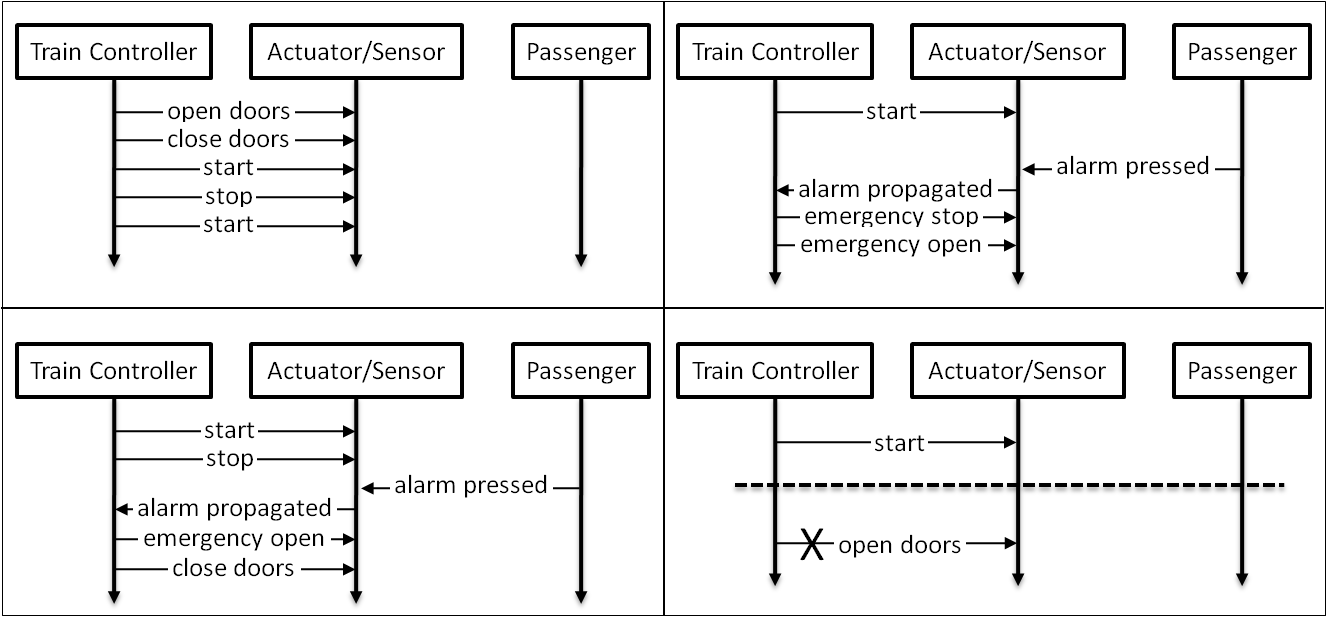
\includegraphics[trim=3mm 3mm 3mm 3mm, clip]{src/4-inductive/images/four-initial-scenarios}}
\caption{Initial positive and negative scenarios for a train system\label{Fig:init:scen}.}
\end{figure}


\item[ChooseStatePair] The candidate solution is refined by merging well- selected state pairs. The \texttt{ChooseStatePair} function determines which pairs to consider. It relies on the standard order $<$ on strings. Each state of the PTA can be labeled by its unique prefix from the initial state. Since prefixes can be sorted according to that order, the states can be ranked accordingly. For example, the PTA states in Fig.~\ref{Fig:algo:steps} are labeled by their rank according to this order. The algorithm considers states $q$ of the PTA in increasing order. The state pairs considered for merging only involve such state $q$ and any state $q'$ of lower rank. The $q'$ states are considered in increasing order as well. This particular ordering is specific to the original RPNI algorithm.

\item[Merge] The \texttt{Merge} function merges the two states $(q, q')$ selected in order to compute a quotient automaton, that is, to generalize the current set of positive behaviors. In the example of Fig.~\ref{Fig:algo:steps}, we assume that states 0, 1, and 2 were previously determined not to be compatible for merging (through negative scenarios initially submitted or generated scenarios that were rejected by the user). Merging a candidate state pair may produce a non-deterministic LTS. For example, after having merged $q = 3$ and $q' = 0$ in the upper part of Fig.~\ref{Fig:algo:steps}, two transitions labeled \texttt{start} from state 0 lead to states 2 and 6, respectively. In such a case, the \texttt{Merge} function merges states 2 and 6 and, recursively, any further pair of states that introduces non-determinism. 

We call \textsl{merging for determinization} this recursive operation of removing non-determinism. This operation guarantees that the current solution at any step is deterministic. It produces an automaton which may accept a more general language than the one it starts from. Therefore, it is not equivalent to the standard algorithm to transform a non deterministic automaton into a deterministic one accepting the same language~\cite{Hopcroft:1979}. Notably, the time complexity of merging for determinization is a linear function of the number of states of the automaton it starts from whereas the standard determinization algorithm is exponential in the worst case. Also, the resulting automaton is still part of the same inductive search space (see Section~\ref{subsection:gi-background-search-space}). 

\begin{figure}
\centering
\scalebox{.67}{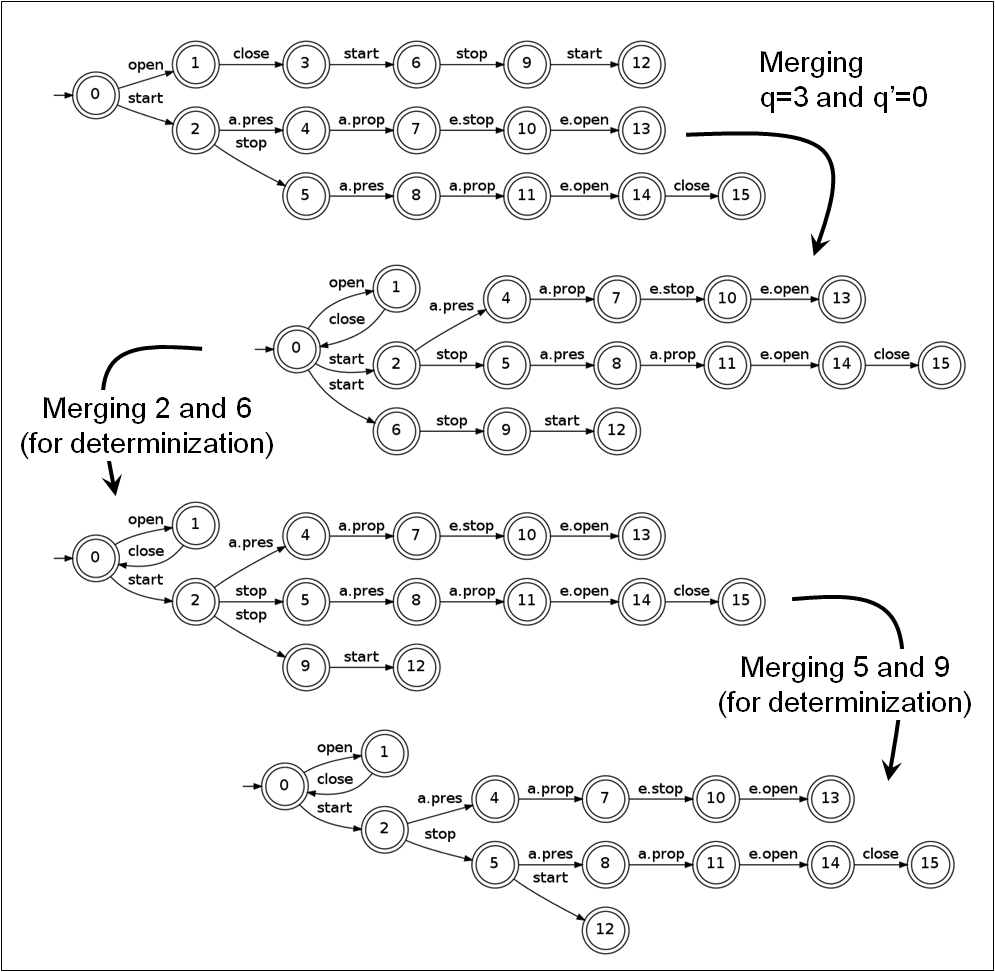
\includegraphics[trim=3mm 3mm 3mm 3mm, clip]{src/4-inductive/images/algo-steps}}
\caption{A typical induction step of the \textsc{QSM} algorithm\label{Fig:algo:steps}.}
\end{figure}

When two states are merged, the rank of the resulting state is defined as the lowest rank of the pair; in particular, the rank of the merged state when merging $q$ and $q'$ is defined as the rank of $q'$ by construction. If no compatible merging can be found between $q$ and any of its predecessor states according to $<$, state $q$ is said to be \textsl{consolidated}. In the example, states 0, 1, and 2 are consolidated.

\item[Consistent] The \texttt{Consistent} function checks whether the automaton $A_{new}$ correctly rejects all negative scenarios. As seen in the pseudo code, the quotient automaton is discarded by \textsc{QSM} when it is detected not to be consistent.

\end{description}

\subsection{Generating queries submitted to the end-user\label{QSM:query}}

This section describes how queries are generated in the \textsc{QSM} algorithm and how the answers provided by the end-user are processed.

\begin{description}

\item[GenerateQuery] When an intermediate solution is consistent with the available scenarios, new scenarios are generated for classification by the end-user as positive or negative. The aim is to avoid poor generalizations by enriching the possibly limited collection of initial scenarios. The notion of characteristic sample drives the identification of which new scenarios should be generated as queries. 

Recall from section~\ref{subsection:gi-background-rpni} that a sample is characteristic of a regular language $L$ if it contains enough positive and negative information. On the one hand, the required positive information is the set of short prefixes $Sp(L)$ which form the shortest histories leading to each state of the canonical automaton $A(L)$. This positive information must also include all elements of the kernel $N(L)$ which represents all system transitions, that is, all shortest histories followed by any admissible event. If such positive information is available, $A(L)$ can always be derived from the PTA by an appropriate set of merging operations. On the other hand, the negative traces provide the necessary information to make incompatible the merging of states which should be kept distinct. A negative trace which would exclude the merging of a state pair $(q, q')$ can be simply made of the shortest history leading to $q'$ followed by any continuation from state $q$ as detailed below.

Consider the current solution of our induction algorithm when a pair of states $(q, q')$ is selected for merging (line 5 in the pseudo code). By construction, $q'$ is always a consolidated state at this step of the algorithm; that is, $q'$ is considered to be in $Sp(L)$. State $q$ is always both the root of a tree and the child of a consolidated state. In other words, $q$ is situated at one letter of a consolidated state, that is, $q$ is considered to be in $N(L)$. States $q$ and $q'$ are compatible according to the available negative scenarios; they would be merged by the standard RPNI algorithm. The QSM extension will first confirm or infirm the compatibility of $q$ and $q'$ by generating scenarios to be classified by the end-user. The generated scenarios are constructed as follows.

\begin{figure}
\centering
\scalebox{.75}{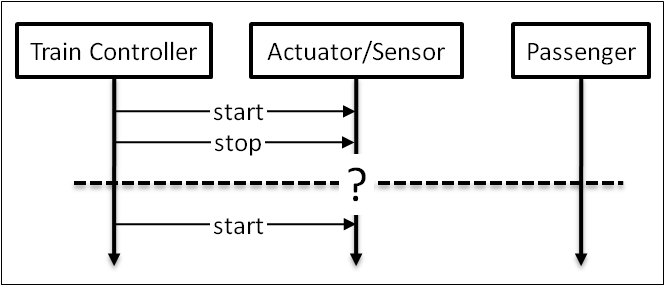
\includegraphics[trim=3mm 3mm 3mm 3mm, clip]{src/4-inductive/images/scenario-question}}
\caption{A new scenario to be classified by the end-user\label{Fig:generated:question}.}
\end{figure}

Let $A$ denote the current solution, $L(A)$ the language generated by $A$, and $A_{new}$ the quotient automaton computed by the \texttt{Merge} function at some given step. Let $x \in Sp(L)$ and $y \in N(L)$ denote the short prefixes of $q'$ and $q$ in A, respectively. Let $u \in L(A)/y$ denote a suffix of $q$ in $A$. 

A generated scenario is built from a system trace $xu$ such that $xu \in L(A_{new})\setminus L(A)$; it can be further decomposed as $xvw$ such that $xv \in L(A)$. The trace $xu$ is thus constructed as the short prefix of $q'$ concatenated with a suffix of $q$ in the current solution, provided the entire behavior is not yet accepted by $A$. Such system trace can be converted to MSC using the structural information provided by a context diagram \cite{Jackson:1995}. The scenario is made of two parts: the first part $xv$ is an already accepted behavior whereas the second part $w$ provides a continuation to be checked for acceptance by the end-user. When submitted to the end-user, the generated scenario can always be rephrased as a question: after having executed the first episode ($xv$), can the system continue with the second episode ($w$)? 

Consider the example in Fig.~\ref{Fig:algo:steps} with selected state pair $q=3, q'=0$. As $q'$ is the root of the PTA, its short prefix is the empty trace $\lambda$. The suffixes of $q$ here yield one generated question (Fig.~\ref{Fig:generated:question}), which can be rephrased as follows: when having started and stopped the train, can the controller restart it? One can see that the first episode of this scenario in Fig.~\ref{Fig:algo:steps} is already accepted by $A$ whereas the entire behavior is accepted in $A_{new}$.

\item[CheckWithEndUser] When a new scenario is generated, it is submitted as a query to the end-user. If the end-user classifies the $Query$ as positive, it is added to the collection of positive scenarios. This addition changes the search space as it extends $S^+$ and consequently the PTA. However, this extension is implicit as the new solution $A_{new}$ is, by construction, also a quotient automaton of this extended PTA. When the $Query$ is classified as negative the induction process is recursively started on the extended scenario collection.

\end{description}

The QSM algorithm has a polynomial time complexity in the size of the learning sample $\mathcal{L}^+(Sc)$, see \cite{Dupont:2008}. 

Moreover, when it receives a characteristic sample in the initial scenario collection it is guaranteed that no additional scenario can be classified as negative. It follows that QSM will not be called recursively anymore and stops by returning the target model. 

An experimental study of the actual sample size required to observe the convergence of \textsc{QSM} and the number of queries submitted to the end-user is detailed in Chapter~\ref{chapter:evaluation}.

\subsection{Reducing the number of queries; the blue-fringe optimization\label{BlueFringe}}

The order in which states are considered for merging by the \texttt{ChooseStatePair} function described in section~\ref{QSM:merging} follows from the implicit assumption that the current sample is characteristic. Consequently, two states are considered compatible for merging if there is no suffix to distinguish among them. This can lead to a significant number of scenarios being generated to the end-user when the initial sample is sparse and actually not characteristic for the target System LTS. 

To overcome this problem, one can use an optimized strategy known as Blue-Fringe~\cite{Lang:1998}. The difference lies in the way state pairs are considered for merging. The general idea is to early detect incompatible state pairs and, subsequently, first consider state pairs for which compatibility has the highest chance to be confirmed by the user through positive classification. The resulting ``please confirm'' interaction may also appear more appealing to the user.

\begin{figure}
\centering
\scalebox{.55}{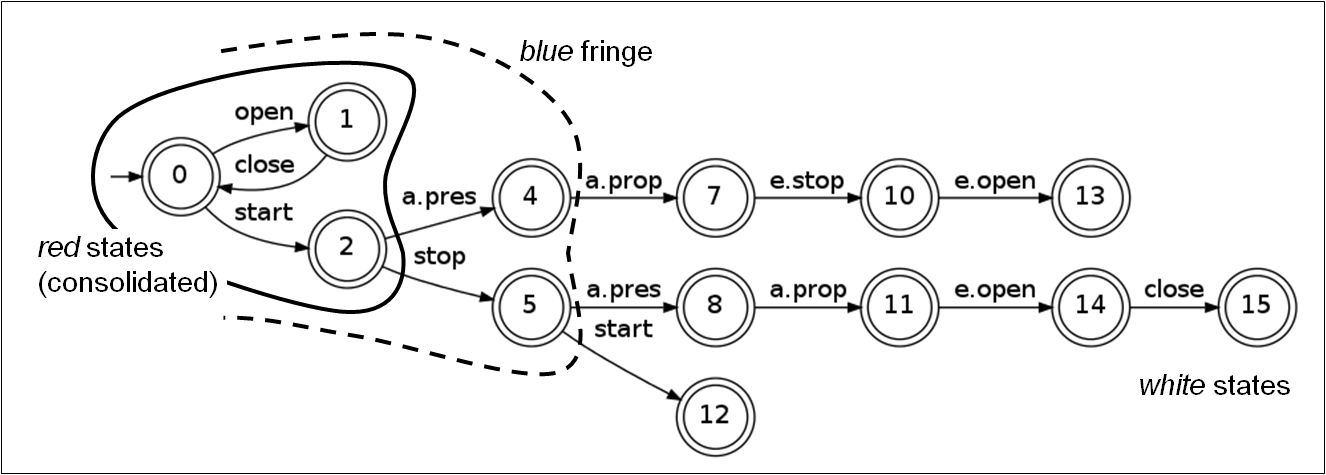
\includegraphics[trim=3mm 3mm 3mm 3mm, clip]{src/4-inductive/images/blue-fringe}}
\caption{Consolidated states (red) and states on the fringe (blue) in a temporary solution\label{Fig:BlueFringe}.}
\end{figure}

Fig.~\ref{Fig:BlueFringe} gives a typical example of a temporary solution produced by the original algorithm. Three state classes can be distinguished in this LTS. The red states are the consolidated ones (0, 1 and 2 in this example). Outgoing transitions from red states lead to blue states unless the latter have already been labeled as red. Blue states form the blue fringe (4 and 5 in this case). All other states are white states. 

The original \texttt{ChooseStatePair} function described in section~\ref{QSM:merging} considers the lowest-rank blue state first (state 4 here) for merge with the lowest-rank red state (0). When this choice leads to a compatible quotient automaton, generated scenarios are submitted to the end-user; in this case, a scenario equivalent to the trace \artifact{<alarm propagated, emergency stop, emergency open>}. The above strategy may lead to multiple queries being generated to avoid poor generalization. Moreover, such queries may be non-intuitive for the user, \textit{e.g.} the \artifact{alarm propagated} event is sent to the train controller without having been fired by the \artifact{alarm pressed} event to the sensor.

To select a state pair for merging, the Blue-Fringe strategy evaluates all (red, blue) state pairs first. The \texttt{ChooseStatePair} function now calls the \texttt{Merge} and \texttt{Compatible} functions before selecting the next state pair. If a blue state is found to be incompatible with all current red states, it is immediately promoted to red; the blue fringe is updated accordingly and the process of evaluating all (red, blue) pairs is iterated. When no blue state is found to be incompatible with red states, the most compatible (red, blue) pair is selected for merging. This is dictated by a scoring mechanism implemented in the \texttt{Compatible} function (see below).

For implementing the Blue-Fringe strategy, it is convenient to adapt \texttt{Initialize} so as to build an \emph{augmented} prefix tree acceptor. Such PTA captures the negative traces in $\mathcal{L}^-(Sc)$ in addition to the positive traces in $\mathcal{L}^+(Sc)$. States reached by a negative trace are tagged as error states; they are depicted in black, as in Fig. \ref{figure:augmented-pta}. 

The \texttt{Compatible} function is also updated to return a compatibility score instead of a boolean value. The score is defined as $-\infty$ when merging the current (red, blue) pair leads to merge an accepting state and an error state during merging for determinization\footnote{in the case of a prefix-closed language, non-error states are all accepting. Recall that this is not necessarily true for any regular language.}; this score indicates an incompatible merging. Otherwise, the compatibility score measures how many accepting states have been merged together. The (red, blue) pair with the highest compatibility score is considered first. The strategy can be further refined with a compatibility threshold $\alpha$ as additional input parameter. Two states are considered to be compatible if their compatibility score is above that threshold. This additional parameter controls the level of generalization since increasing $\alpha$ decreases the number of state pairs that are considered compatible for merging; it thus decreases the number of generated queries.

\begin{figure}\centering
\scalebox{.35}{\includegraphics*{src/4-inductive/images/augmented-pta}}
\caption{Augmented PTA for scenarios in Fig.~\ref{Fig:init:scen}\label{figure:augmented-pta}.}
\end{figure}

Experimental results about the effectiveness of using QSM with and without the Blue-Fringe strategy are detailed in Chapter~\ref{chapter:evaluation}.

\section{Using constraints for multi-view consistency\label{section:inductive-mutliview-consistency}}

The interactive QSM algorithm described in Section~\ref{section:lts-induction-from-mscs} provides a system LTS consistent with all available positive and negative scenarios. The Blue-Fringe strategy can also be applied to reduce the number of additional scenarios submitted to the end-user. The latter strategy relies on two equivalence classes partitioning the states of an augmented PTA. These classes correspond to the accepting states and the error states, respectively. All states belonging to the same class are not necessarily merged in the final solution; however, the \texttt{Compatible} function guarantees that only states belonging to the same class \emph{can} be merged.

This approach can be extended to achieve multi-view consistency by incorporating various sources of information. Such information refines the equivalence partition and further constrains the compatible merging operations. Injecting knowledge-based constraints has many advantages: 
\begin{itemize}
\item It ensures strong consistency of the system LTS with other views;
\item It reduces the number of scenario queries in the interactive setting;
\item It speeds up the search.
\end{itemize}

Section \ref{subsection:induction-pruning-with-domain-knowledge} shows how to incorporate domain knowledge such as fluent definitions. Section \ref{subsection:induction-pruning-with-goals} shows how goals can be used to constrain the generalization. 

The optimization techniques detailed hereafter are based on various equivalence relations over system states. The term \emph{equivalence relation} is used here in its usual mathematical sense, namely, a symmetric, reflexive, and transitive binary relation over states. The general principle underlying our techniques is the following:
\begin{quote}
\emph{Two states will be considered for merging if they agree according to all considered equivalence relations.}
\end{quote}

%%%%%

\subsection{Injecting domain knowledge\label{subsection:induction-pruning-with-domain-knowledge}}

The domain knowledge used to constrain state merging comes from multiple sources: 
\begin{itemize}
\item Fluent definitions;
\item Knowledge about components in the environment of the software-to-be;
\item Specifications of domain properties.
\end{itemize}
We discuss them successively.

%%

\subsubsection*{Propagating fluents}

Fluent definitions provide simple and easy-to-provide domain descriptions to constrain induction. For example, the definition
\begin{center}
fluent $DoorsClosed = \textless \{$close doors$\}, \newline
 \{$open doors, emergency open$\} \textgreater $ initially $true$ \\
\end{center}
describes train door states as being either closed ($DoorsClosed = true$) or open ($DoorsClosed = false$); it also states which event is responsible for which state change. 

Such descriptions can be effectively used to constrain the induction process so that the synthesized System LTS conforms to them. The idea is to decorate each state of the PTA with the value of every fluent. This can be done using a symbolic execution algorithm \cite{Damas:2006, Damas:2011} (see Section~\ref{section:background-fluents}).

The pruning rule for constraining the induction process is here to \emph{avoid merging inconsistent states} according to these decorations. 

The specific equivalence relation is thus the set of state pairs where both states have the same fluent value assignment. The decoration of the merged state is simply inherited from the states being merged.
\begin{quote}
\emph{Two states will be considered for merging if they have the same value for every fluent.}
\end{quote}

Fig.~\ref{dc-augmented-pta} shows the result of propagating the values of the fluent \emph{DoorsClosed} along the augmented PTA built from the scenarios described in Fig.~\ref{Fig:init:scen}.

\begin{figure}
\centering
\scalebox{.33}{\includegraphics*{src/4-inductive/images/dc-augmented-pta}}
\caption{Propagating fluents along the PTA to prune the inductive search space\label{dc-augmented-pta} (DC stands for \emph{DoorsClosed})}
\end{figure}

%%

\subsubsection*{Unfolding models of external components}

Quite often the components being modeled need to interact with other components in their environment - \textit{e.g.}, legacy components in a bigger existing system, foreign components in an open system, etc. In such cases the behavior of external components is generally known - typically, through some behavioral model \cite{Hall:2004}. External components are assumed here to be known by their LTS model. 

For example, Fig.~\ref{Fig.:alarm-sensor} shows the LTS for a legacy alarm sensor in our train system. When the alarm button is pressed by a passenger, this component propagates a corresponding signal to the train controller. 

\begin{figure}
\centering
\scalebox{.4}{\includegraphics*{src/4-inductive/images/alarm-sensor}}
\caption{LTS model for an alarm sensor\label{Fig.:alarm-sensor}.}
\end{figure}

A LTS model of an external component can constrain the induction process so that the synthesized system LTS conforms to it. The idea is to decorate the PTA with states of the external LTS by unfolding the latter onto the PTA. Such decoration is performed by jointly visiting the PTA and the external LTS; the latter synchronizes on shared events and remains in its current state on other events.

Fig.~\ref{Fig.:alarm-unfolded-pta} shows the result of unfolding the alarm sensor LTS from Fig.~\ref{Fig.:alarm-sensor} on the augmented PTA built from the scenarios described in Fig.~\ref{Fig:init:scen}. Each state of the PTA is labeled with the number of the corresponding state in the alarm sensor LTS. 

\begin{figure}
\centering
\scalebox{.35}{\includegraphics*{src/4-inductive/images/alarm-unfolded-pta}}
\caption{Unfolding the alarm sensor LTS onto the PTA\label{Fig.:alarm-unfolded-pta}.}
\end{figure}

The pruning rule for constraining the induction process is now to \emph{avoid merging states decorated with distinct states of the external component}. The specific equivalence relation used here is the set of states where both states have the same external LTS state. 

\begin{quote}
\emph{Two states will be considered for merging if they have the same external LTS state.}
\end{quote}

%%

\subsubsection*{Using declarative domain properties}

Descriptive statements and assumptions about the domain can be expressed declaratively in FLTL (see Section~\ref{section:background-goals}). For example, the physical law
\begin{align*}
\square(HighSpeed \rightarrow Moving)
\end{align*}
\noindent excludes all negative traces where the train is running at high speed while not moving. 

The technique for constraining induction through descriptive or prescriptive statements is the same; we discuss it hereafter.

%%%%%

\subsection{Injecting goals\label{subsection:induction-pruning-with-goals}}

For reasons discussed in Section \ref{section:background-goals}, we restrict our attention to goals and domain properties that can be formalized as pure FLTL safety properties. Remember that these properties refer to  ``\emph{something bad may never happen}''.

Consider the following goal requiring train doors to remain closed while the train is moving:
\begin{center}
\artifact{Maintain[DoorsClosed While Moving]} = $\square(Moving \rightarrow DoorsClosed)$
\end{center}

Fig.~\ref{Fig.:tester-automaton-inductive} shows the tester automaton for this property (cfr. Section \ref{subsection:background-property-and-tester-automata}). The accepting state of this tester captures all traces violating the safety property; any trace leading to it corresponds to an undesired system behavior. In particular, the trace \artifact{<start, open>} corresponds to the initial negative scenario in Fig.~\ref{Fig:init:scen}. As seen in Fig.~\ref{Fig.:tester-automaton-inductive}, the tester provides many more negative traces. Property testers can in fact provide potentially infinite classes of negative scenarios.

\begin{figure}
\centering
\scalebox{.35}{\includegraphics*{src/4-inductive/images/tester-automaton}}
\caption{Tester LTS for the goal \artifact{Maintain[DoorsClosed While Moving]}.\label{Fig.:tester-automaton-inductive}}
\end{figure}

The property tester is used to constrain the induction process in a way similar to an external component LTS. The PTA and the tester are traversed jointly in order to decorate each PTA state with the corresponding tester state. Fig.~\ref{Fig.:goal-unfolded-pta} shows the PTA decorated using the tester of Fig.~\ref{Fig.:tester-automaton-inductive}.

\begin{figure}
\centering
\scalebox{.35}{\includegraphics*{src/4-inductive/images/goal-unfolded-pta}}
\caption{Augmented PTA decorated using the tester automaton from Fig.~\ref{Fig.:tester-automaton-inductive}\label{Fig.:goal-unfolded-pta}.}
\end{figure}

The pruning rule for constraining the induction process is now to \emph{avoid merging states decorated with distinct states of the property tester}. The specific equivalence relation used here is the set of states where both states correspond to the same state of the property tester. 
\begin{quote}
\emph{Two states will be considered for merging if they have the same property tester state.}
\end{quote}

This pruning technique guarantees the consistency between the synthesized System LTS and the considered goals and domain properties. In other words, for every goal or domain property $G$ injected in the synthesis process, the following consistency condition holds (see Section \ref{subsection:background-goals-consistency}):
\begin{align*}
\mathcal{L}^-(G) \cap \mathcal{L}(System) &= \emptyset,
\end{align*}
where \emph{System} here denotes the synthesized system LTS and $\mathcal{L}^-(G)$ captures all traces violating $G$.

Note that the guarantee given by the above condition is weaker than the \emph{consistent system view} condition (\ref{relation:inductive-statement-negative}) in Section \ref{subsection:inductive-synthesis-statement}. The latter requires the consistency of the synthesized system $\system$ while the above condition only applies to the system LTS. As with implied negative scenarios, a goal could be satisfied by the synthesized System LTS while being violated by the real distributed system. This issue is further discussed in Section \ref{section:inductive-discussion}.

\subsection{Discussion\label{subsection:qsm-constraints-implementation-notes}}

The equivalence relations considered in the previous sections are all invariant under state merging. In other words, a state derived by merging some states simply inherits their relation. This allows each relation to be computed only once on the initial PTA; the results of such pre-processing are kept as annotations on PTA states. 

Our implementation reuses the decoration algorithm from \cite{Damas:2006} to propagate fluent values on the PTA (see Section~\ref{subsection:fluents-along-multiple-traces}). Its generalization in~\cite{Damas:2011} may be used as an effective mean to unfold models of legacy components and tester automata on the PTA without additional developments.

The principle for constraining state merging through equivalence relations first appeared in~\cite{Coste:1998, Coste:2004}. It can be further instantiated to other equivalence relations not considered here. In particular, it is \emph{not} limited to relations that are invariant under state merging.

As an illustrative example, consider the following generalization of the way fluent values are used to constrain the induction process. We know from Section~\ref{subsection:fluents-along-multiple-traces} that the states of any LTS can be annotated with invariants defined on fluents. Let $inv$ denote the function mapping each PTA state to its state invariant; let also denote by \emph{Dom} a domain property that must be met in every state of the system LTS. Consider the following pruning rule:
\begin{quote}
\emph{Two states $q$ and $q'$ will be considered for merging if $inv(q) \wedge inv(q') \models \mbox{Dom}$}
\end{quote}

The equivalence relation here is the set of state pairs whose conjunction of invariants satisfies the domain property. This equivalence relation is \emph{not} invariant under state merging. The merging constraint can however be enforced; to achieve this, the compound state resulting from merging $q$ and $q'$ has to be annotated by the conjunction of their state invariants; this new invariant is then used in subsequent state merging.

In the general case of DFA induction\footnote{that is, in contrast to LTS induction}, a similar mechanism is needed to implement the Blue-fringe optimization with an augmented PTA. In that case, an error state may be merged with a non accepting state provided the result is not merged later with an accepting one. That is, the relation capturing the equivalence of states in terms of their continations is not invariant under state merging.

\section{LTS synthesis from high-level MSCs\label{section:inductive-from-hMSC}}

The previous sections have shown how system behaviors specified in collections of MSC scenarios can be first generalized as a System LTS, then decomposed as a set of agent LTSs. The technique supports the incremental enrichment of an initial scenario collection through scenario queries. It also takes other models into account, such as goals, so as to preserve multi-view consistency. Behavior generalization, incremental synthesis and multi-view consistency are the three main requirements identified in Section \ref{subsection:inductive-synthesis-requirements}. 

Coupled with other synthesis techniques such as goal mining from scenarios\footnote{whose simplest form consists in asking ``why'' when facing with a negative scenario.} \cite{Damas:2006}, interactive LTS induction is really effective; starting from a small initial scenario collection, richer system models can be synthesized in only a few iterations. Chapters~\ref{chapter:evaluation} and \ref{chapter:tool-support} illustrate this claim with evaluations and overview of the tool support.

However, for any non-toy system, a large scenario collection might become unmanageable. Among others, consistency of the collection might be difficult to guarantee without costly refactoring on scenarios. One reason is that all scenarios of a collection are required to start in the same system state; this usually implies a lot of redundancy in system descriptions.

One way to tackle this problem is to use high-level message sequence charts (hMSCs) for structuring scenario descriptions. As detailed in Section \ref{subsection:background-hmsc}, hMSCs are directed graphs where each node refers to a MSC or a finer grained hMSC (see Fig.~\ref{image:train-hmsc}). Scenarios can then be structured by introducing alternatives, sequences and loops.

Having a structured form of scenario \emph{helps} specifying a large system with scenarios; it does not \emph{solves} the problem of achieving a complete and consistent view of agent behaviors:
\begin{itemize}
\item capturing all possible interleavings of a distributed system proves difficult with scenarios; a hMSC is therefore hardly complete in practice,
\item complementary features of a system deserve being specified in complementary models; in addition to using multiple system views, having system behaviors specified in more than one hMSC makes sense.
\end{itemize}

Having a synthesis technique to merge and to generalize behaviors described in hMSCs seems a convenient extension to the synthesis technique described so far. For this, the LTS synthesis statement is first revisited in Section~\ref{subsection:hmsc-induction-problem-revisited}. The inductive algorithm is then adapted in Section \ref{subsection:hmsc-induction-algo-adaptation}.

\subsection{Revisiting the LTS synthesis statement\label{subsection:hmsc-induction-problem-revisited}}

Merging multiple hMSCs $H_1,\ldots,H_n$ with respect to trace behaviors simply amounts to compute the union of their respective languages. This is equivalent to building a new hMSC $H$ reaching the finer-grained $H_1,\ldots,H_n$ from its initial state. Additional positive scenarios $S^+_1,\ldots,S^+_n$, typically coming from scenario queries, could be integrated in a similar way. This is illustrated in Fig.~\ref{figure:multiple-hmscs}.

\begin{figure}\centering
\scalebox{.70}{
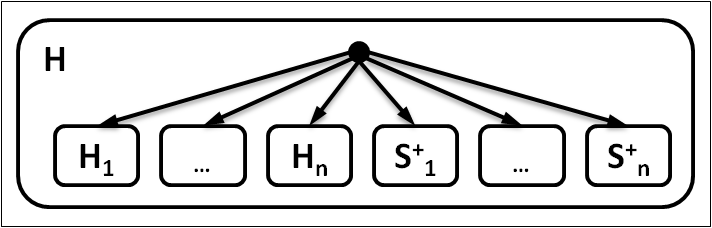
\includegraphics[trim=3mm 3mm 3mm 3mm, clip]{src/4-inductive/images/multiple-hmscs}}
\caption{Merging multiple hMSCs amounts to builds a new one that reaches finer-grained hMSCs from its initial state.\label{figure:multiple-hmscs}} 
\end{figure}

However, a hMSC only permits specifying positive behaviors. As explained in previous sections, negative information is needed to avoid poor generalizations. Negative scenarios, fluents, goals, etc. all provide a source of negative knowledge that can be used to constraint the induction process. The algorithmic adaptations considered later stay compatible with the constraint mechanism based on equivalence relations on system states.

Without loss of generality therefore, we will assume that behaviors are specified through one hMSC only, complemented with a scenario collection. The latter contains negative scenarios and answers to scenario queries. Under these assumptions, the LTS synthesis statement is restated as follows: 

\begin{quote}
\underline{Given}~a hMSC $H$ and a scenario collection $Sc = (S^+,S^-)$ consistent with each other
\begin{align*}
[\mathcal{L}^+(Sc) \cup \mathcal{L}(H)] \cap \mathcal{L}^-(Sc) &= \emptyset
\end{align*}
\underline{Synthesize}~the system as a composition of agent LTSs
\begin{align*}
System = (Ag_1 \parallel \ldots \parallel Ag_n)
\end{align*}
\underline{Such that}~$H$, $Sc$ and $System$ are consistent.
\end{quote}

The hMSC trace semantics is left open in the formulation above. In other words, one has to decide which set of behaviors does $\mathcal{L}(H)$ denote. We recall below the relations between the three hMSC languages covered in Section \ref{subsection:background-hmsc}: 
\begin{align}
\mathcal{L}_{strong}(H) \subseteq \mathcal{L}_{weak}(H) &\subseteq \mathcal{L}_{arch}(H)
\end{align}

$\mathcal{L}_{strong}(H)$ denotes the set of system behaviors with strong sequential composition of hMSC nodes and total event ordering inside MSCs. It is the simplest and most intuitive model for stakeholders involved in early phases of system design. However, it supposes an implicit synchronization scheme used by the agents that is usually not available in real distributed systems. $\mathcal{L}_{arch}(H)$ is the most realistic for such systems, as it captures all possible interleavings of agent behaviors. $\mathcal{L}_{weak}(H)$ is mainly used for explaining and detecting implied scenarios in hMSC specifications \cite{Uchitel:2003}; it is also the hardest to compute.

Making a choice of semantics is required for generalizing behaviors because inductive synthesis takes a set of traces as input. The chosen semantics must of course fit domain assumptions. From an algorithmic point of view however, the three hMSC languages above require the same adaptations of the inductive process, as explained in the next sections.

\subsection{Generalizing high-level MSC languages\label{subsection:hmsc-induction-algo-adaptation}}

Recall that learning a regular language $L$ aims at generalizing a positive sample $S_+$ under the control of a negative sample $S_-$ such that the following relation of language inclusions holds:
\begin{align}
S_+~~\subseteq~~L~~\subseteq~~\Sigma^*\setminus S_-
\end{align}

LTS synthesis from a scenario collection $Sc$ reduces to grammar induction because the sets $\mathcal{L}^+(Sc)$ and $\mathcal{L}^-(Sc)$ are valid positive and negative samples, respectively (see Section \ref{subsection:inductive-lts-synthesis-reduction}). In particular, they denote \emph{finite} sets of traces.

When considering the generalization of hMSC behaviors, the sets of positive and negative traces are $\mathcal{L}^+(Sc) \cup \mathcal{L}(H)$ and $\mathcal{L}^-(Sc)$, respectively. The positive set is no longer a sample because $\mathcal{L}(H)$ might contain an infinite number of traces. Therefore, the current problem statement no longer fits exactly in the identification in the limit framework presented in Section \ref{section:inductive-background}. 

From a theoretical point of view, it means that generalizing hMSC languages is a different problem than generalizing MSC languages; therefore, further study would be needed to re-state the convergence criteria and the notion of characteristic sample in particular. From an algorithmic point of view, however, only a few adaptations of RPNI and QSM are required. They are explained in the next section.

\subsection{The Automaton State Merging algorithm\label{subsection:automaton-state-merging}}

The algorithm to generalize behaviors specified in a hMSC is given in Algorithm~\ref{ASM}, called Automaton State Merging (ASM). It is very similar to QSM, given in Section~\ref{section:lts-induction-from-mscs}, except that the interactive feature is ommited here (we discuss it later). QSM itself being an interactive extension to RPNI, Algorithm~\ref{ASM} is almost RPNI itself which might appear suprising at first glance.

\begin{algorithm}
{
\vspace{0.2cm}
\KwIn{A high-level MSC $H$ and a scenario collection $Sc = (S_+, S_-)$}
\KwOut{A System LTS, consistent with both $H$ and $Sc$}

$A \leftarrow $ {\tt Initialize($H$, $Sc$)}\\
\While{$(q,q') \leftarrow $ {\tt ChooseStatePair($A$)}}{
$A_{new} \leftarrow$ {\tt Merge$(A,q,q')$}\\
\If{{\tt Consistent$(A_{new}, S_-)$}}{
 $A \leftarrow A_{new}$
}
}
\Return{$A$}}
\vspace{0.2cm}
\caption{\textsc{ASM}, a state-merging algorithm from high-level Message Sequence Charts\label{ASM}}
\end{algorithm}

The main difference between RPNI and QSM on one side and ASM on the other side is the initial automaton solution built by \texttt{Initialize}. RPNI and QSM initially convert the input \emph{sample} as a PTA, hence a tree, whereas ASM converts the input \emph{language} of the hMSC as a DFA, hence an graph. The main loop of the ASM algorithm can then be seen as generalizing any regular language, under the control of a negative sample; hence the ``Automaton State Merging'' name. A few adaptations are however required to the different functions of the algorithm: 

\begin{description}

\item[Initialize] This function is adapted to return a DFA instead of a PTA. On one side, the positive traces from the hMSC may be captured through a LTS as discussed in Section \ref{subsection:background-hmsc}, provided a choice of hMSC semantics. On the other side, the scenario collection can be captured through a PTA. These two automata can be merged through standard algorithms for capturing the union of regular languages \cite{Hopcroft:1979}. 

In order to use the Blue-Fringe heuristic (see below), the obtained DFA may be augmented with error states encoding the negative sample given by $S_-$. 

\item[ChooseStatePair] In order to preserve the merging order used by RPNI, this function must be slightly adapted. The idea is to pre-compute the natural order among the states of the initial DFA solution. A breadth first search is used and each of them is numbered when encountered. 

Not that the Blue-Fringe strategy does not require special support. The distinction between red and blue states does not rely on any assumption about the initial solution being a tree; in particular, the fact that a fringe state is the root of a tree in RPNI and QSM is incidental (see \texttt{Merge} below).

\item[Merge] The merging for determinization process is often implemented assuming a tree invariant property. This property states that, when considering two states to be merged, at least one of them is the root of a tree. Such a property holds for RPNI and QSM, even when the Blue-Fringe optimization is used. It is a sufficient condition for the determinization process to be finite. 

Even though it is convenient, the tree invariant property is not required, as explained in \cite{Lambeau:2008}. The main merging loop and the \texttt{Merge} function can be implemented without the tree invariant property because the recursive determinization process stops naturally on the first DFA encountered. This observation allows one to start from an arbitrary DFA and, as soon as non-determinism occurs, to reduce it. 
%Fig.~\ref{figure:merging-for-determ-on-dfa} gives an example of such a recursive operation.

\end{description}

The interactive feature of QSM could be easily adapted and plugged to ASM. It consist in replaincing the main loop ASM by the one of QSM (see Algorithm~\ref{QSM} in Section~\ref{section:lts-induction-from-mscs}). In the latter, the \texttt{GenerateQuery} function must be adapted as follows:

\begin{description}

\item[GenerateQuery] The generation of scenario queries relies on the tree invariant property mentioned above. When merging a state pair $(q,q')$, a scenario query is built with the shortest trace leading to $q$ concatenated with the suffixes of $q'$. When $q'$ is the root of a tree, generating a finite scenario is straightforward.

If the tree invariant property no longer holds, the \texttt{GenerateQuery} function must be extended with a procedure for extracting finite suffixes from $q'$. This does not introduce any technical issues; for example, pre-computing a spanning tree on the initial DFA would associate finite suffixes to each of its state. However, what forms a ``good'' suffix for convergence and scenario classification by end-users is an open question. As the adapted algorithm no longer fits in the identification in the limit framework, the notion of a characteristic sample would need to be adapted. 

\end{description}

%\begin{figure}\centering
%\scalebox{.34}{
%\includegraphics*{src/4-inductive/images/merging-for-determ-on-dfa}}
%\caption{Recursive determinization process. States \{3\} and \{0\} of an arbitrary DFA are merged, which causes a non-determinism on letter $b$ from state \{0,3\}. The destination states \{2\} and \{4\} are subsequently merged to reduce the non-determinism.\label{figure:merging-for-determ-on-dfa}} 
%\end{figure}

From a grammar induction point of view, the ASM algorithm can be seen as generalizing any positive regular language $\mathcal{L}^+$ under the control of a negative sample $S_-$. As such, RPNI is thus a special case where the positive language forms a sample $S_+$, that is a finite set of strings.

Interrestingly, the constraint mechanism from Section~\ref{section:inductive-mutliview-consistency} to prune the induction search space and guarantee multi-view consistency can still be used with ASM. Indeed, the partitionning of PTA states according to equivalence relations extracted from domain knowledge can be performed on the input DFA returned by \texttt{Initialize}, \emph{mutatis mutandis}. 

In particular, goals and domain properties can still be used to prune the induction search space, as explained in Section~\ref{subsection:induction-pruning-with-goals}. As goals actually capture negative languages through their tester automaton, this amounts to consider yet another generalization of ASM to generalize a positive language $\mathcal{L}^+$ under the control of a negative one $\mathcal{L}^-$. This generalization is called ASM$^*$ and briefly discussed in \cite{Lambeau:2008}.



\section{Correctness\label{section:inductive-correctness}}

Proving the correctness of our synthesis approach amounts to show that the synthesized system is consistent with both the scenarios and all domain knowledge taken in input. We discuss proof arguments for the different algorithm settings, starting with the simplest case of RPNI-based synthesis and gradually integrating features such as scenario questions and injection of domain knowledge.

\begin{figure}\centering
\scalebox{.65}{
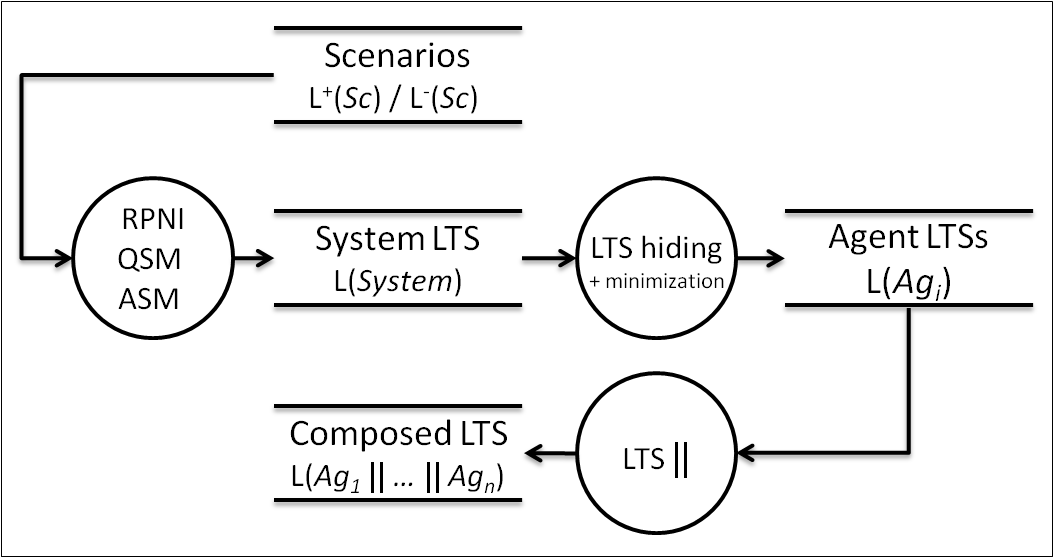
\includegraphics[trim=3mm 3mm 3mm 3mm, clip]{src/4-inductive/images/synthesis-flow-model}}
\caption{Inductive synthesis steps and products.\label{figure:synthesis-flow-model}} 
\end{figure}

Fig.~\ref{figure:synthesis-flow-model} summarizes our approach by showing used algorithms together with their input/output in terms of behavior models and associated languages. 
\begin{itemize}
\item From scenarios, a system LTS is inferred using either RPNI, QSM or ASM. 
\item LTS hiding and minimization is then used to obtain a canonical state machine for each agent. 
\item From the system view point, the result of our synthesis approach is precisely captured by the composition of those state machines.
\end{itemize}

In this figure and in the following discussions,
\begin{itemize}
\item $Sc = (S^+,S^-)$ denotes the input scenario collection; its positive and negative languages are denoted by $\mathcal{L}^+(Sc)$ and $\mathcal{L}^-(Sc)$, respectively.
\item $\mathcal{L}(\me{System})$ denotes the language captured by the inferred system LTS.
\item $\mathcal{L}(Ag)$ denotes the language of an arbitrary agent $Ag$, as captured by its LTS state machine.
\item $\mathcal{L}(\agentscomposed)$ denotes the language captured by the LTS resulting of the composition of individual agent LTSs.
\end{itemize}

We first restrict our attention to the simplest, non-interactive, RPNI approach. Remember from Section~\ref{subsection:inductive-synthesis-statement} that the specification on our approach requires three conditions to hold on synthesized state machines:
\begin{itemize}
\item The \emph{structural consistency} condition requires input scenarios and synthesized agent state machines to agree on the respective agent interfaces.
\item The \emph{consistent agent view} condition requires each synthesized agent state machine to cover the positive behaviors along the corresponding timeline in the input scenarios.
\begin{align}
\mathcal{L}^+(Sc_{\downarrow Ag}) \subseteq \mathcal{L}(Ag)\mbox{~for each agent $Ag$}\label{proof:consistent-agent-view}
\end{align}
where $Sc_{\downarrow Ag}$ denotes the positive behaviors along $Ag$'s timeline in a scenario collection $Sc = (S^+, S^-)$:
\begin{align}
\mathcal{L}^+(Sc_{\downarrow Ag}) = \bigcup_{P \in S^+} \mathcal{L}(P_{\downarrow Ag})~~\cup~~\bigcup_{N \in S^{-}} \mathcal{L}^{+}(N_{\downarrow Ag})\label{proof:lemma-sc-projection}
\end{align}

This is a a slight generalization of the concept of agent traces along a single scenario timeline $M_{\downarrow Ag}$, introduced in Section~\ref{section:background-scenarios}. Observe that it takes both positive and negative scenarios into account.
\item The \emph{consistent system view} requires the system to cover all positive scenarios and reject all negative ones. 
\begin{align}
&\mathcal{L}^+(Sc) \subseteq \mathcal{L}(\agentscomposed)\label{proof:consistent-system-view-1}\\
&\mathcal{L}^-(Sc) \cap      \mathcal{L}(\agentscomposed) = \emptyset\label{proof:consistent-system-view-2}
\end{align}
\end{itemize}

Section~\ref{subsection:system-lts-consistency} briefly discusses the consistency of the inferred system LTS with the scenarios. This result is then used in Section~\ref{subsection:consistent-agent-view} to show that the decomposition step meets the ``structural consistency'' and the ``consistent agent view'' conditions. The ``consistent system view'' condition is further discussed in Section~\ref{subsection:consistent-system-view}. The discussion is pursued in the presence of scenario questions in Section~\ref{subsection:proof-with-scenario-questions} and with the injection of domain knowledge in Section~\ref{subsection:proof-with-domain-knowledge}. Section~\ref{subsection:correctness-of-asm} closes this section with a discussion about the correctness of ASM.

%%%

\subsection{Consistency of the system LTS\label{subsection:system-lts-consistency}}

This section demonstrates that RPNI yields a system LTS consistent with the input scenario collection. The pseudo code given in Algo.~\ref{QSM} is used, ignoring the scenario questions (lines 5 to 10).

\begin{theorem}
\label{theorem:system-lts-consistency-with-sc}
The system LTS synthesized by RPNI covers all positive scenarios and rejects all negative ones.
\begin{align*}
&\mathcal{L}^+(Sc) \subseteq \mathcal{L}(System)\\
&\mathcal{L}^-(Sc) \cap      \mathcal{L}(System) = \emptyset
\end{align*}

\begin{proof}
This theorem is proven by induction using the following invariant:
\begin{align}
&\mathcal{L}^+(Sc) \subseteq \mathcal{L}(A_i)\label{inv:system-lts-consistency-with-sc-1}\\
&\mathcal{L}^-(Sc) \cap      \mathcal{L}(A_i) = \emptyset\label{inv:system-lts-consistency-with-sc-2}
\end{align}

\begin{description}
\item[Base:] $A_0$ denotes the PTA returned by \emph{Initialize}.

The PTA is the largest DFA accepting the positive language; a precondition states that input scenarios are consistent. Therefore the following conditions hold, entailing the invariant:
\begin{align}
&\mathcal{L}^+(Sc) =    \mathcal{L}(A_0)\\
&\mathcal{L}^-(Sc) \cap \mathcal{L}(A_0) = \emptyset
\end{align}

\item[Inductive step:] $A_i$ is the quotient automaton denoting the current solution at step $i$.

From a solution $A_i$, the next solution $A_{i+1}$ is computed by the \emph{Merge} function (see line 3 in Algo.~\ref{QSM}). The latter computes a quotient automaton. Definition~\ref{definition:quotient-automaton} guarantees that such quotient automaton may only generalize the language of $A_i$. As the condition~(\ref{inv:system-lts-consistency-with-sc-1}) holds for $A_i$, the following condition holds as well:
\begin{align*}
&\mathcal{L}^+(Sc) \subseteq \mathcal{L}(A_i) \subseteq \mathcal{L}(A_{i+1})
\end{align*}

On an other hand, quotient automata are only kept as next solution if consistent with the negative scenarios (see lines 4 and 11). Therefore, the following condition holds when such solution is kept (line 11):
\begin{align*}
&\mathcal{L}^-(Sc) \cap \mathcal{L}(A_{i+1}) = \emptyset
\end{align*}

\end{description}
\end{proof}
\end{theorem}

A detailed proof of the convergence of RPNI towards the canonical target automaton when it receives a characteristic sample can be found in~\cite{Oncina:1993} in the more general case of transducer learning.

%%%

\subsection{Structural consistency and consistent agent view\label{subsection:consistent-agent-view}}

Given the consistency of the system LTS with the positive and negative scenarios, the decomposition step guarantees that the \emph{structural consistency} and the \emph{consistent agent view} both hold.

Structural consistency only requires the LTS hiding step to make use of adequate agent alphabets, as induced from the scenarios themselves or given by a (consistent) structural model. We do not discuss it further. 

For each agent $Ag$, the ``consistent agent view'' condition (\ref{proof:consistent-agent-view}) can be derived from (\ref{proof:consistent-system-view-1}) using the following properties and definitions:
\begin{align}
&\mathcal{L}(X) \subseteq \mathcal{L}(Y) \implies \mathcal{L}(X \setminus I) \subseteq \mathcal{L}(Y \setminus I) \label{proof-agent-consistency-1}\\
&\mathcal{L}^+(Sc_{\downarrow Ag}) = \mathcal{L}^+(Sc \setminus \Sigma_{Ag}^c)\label{proof-agent-consistency-2}\\
&\mathcal{L}(Ag) = \mathcal{L}(System \setminus \Sigma_{Ag}^c)\label{proof-agent-consistency-3}
\end{align}
where $\Sigma_{Ag}^c$ denotes the set of all system events excluding those of $Ag$'s interface.
\begin{itemize}
\item (\ref{proof-agent-consistency-1}) states that behavior inclusion is preserved under LTS hiding; this property follows from material in Section~\ref{subsection:lts-hiding}. 
\item (\ref{proof-agent-consistency-2}) rewrites the left term of (\ref{proof:consistent-agent-view}) in terms of hiding of scenario behaviors\footnote{using an abuse of notation as the hiding operator is defined on LTS, not on scenarios collections.}. It can be derived from (\ref{proof:lemma-sc-projection}) and the definition of $M_{\downarrow Ag}$ (see Section~\ref{subsection:background-positive-scenarios}). 
\item (\ref{proof-agent-consistency-3}) follows from the definition (\ref{definition:decomposition-step}) of decomposition step itself (see Section~\ref{subsection:inductive-synthesis-approach}). 
\end{itemize}

From Theorem~\ref{theorem:system-lts-consistency-with-sc} ensuring the consistency of the system LTS with input scenarios, the following condition is established thanks to (\ref{proof-agent-consistency-1})
\begin{align}
&\mathcal{L}^+(Sc \setminus \Sigma_{Ag}^c) \subseteq \mathcal{L}(System \setminus \Sigma_{Ag}^c)\label{proof:consistent-agent-view-milestone}
\end{align}

The ``consistent agent view'' condition (\ref{proof:consistent-agent-view}) is established by substituing the right terms of (\ref{proof-agent-consistency-2}) and (\ref{proof-agent-consistency-3}) in (\ref{proof:consistent-agent-view-milestone}).

%%%

\subsection{Consistent system view: the problem of implied scenarios\label{subsection:consistent-system-view}}

This section discusses the correctness of the ``consistent system view'' condition. The conditions related to the positive and negative scenarios are discussed in turn.

\begin{theorem}
The synthesized system covers all positive scenarios.
\begin{align*}
&\mathcal{L}^+(Sc) \subseteq \mathcal{L}(\agentscomposed)
\end{align*}

\begin{proof}
This condition results from two main properties of our approach:
\begin{itemize}
\item The synthesized system LTS covers all positive scenario behaviors, as guaranteed by Theorem~\ref{theorem:system-lts-consistency-with-sc}.
\begin{align*}
&\mathcal{L}^+(Sc) \subseteq \mathcal{L}(System)
\end{align*}
\item Projecting the system LTS on agent alphabets and recomposing their LTS afterwards does not restrict behaviors:
\begin{align*}
&\mathcal{L}(\mbox{System}) \subseteq \mathcal{L}(\agentscomposed)
\end{align*}
This latter condition can be derived from the definition of agent languages (\ref{proof-agent-consistency-3}) and properties of LTS hiding and composition operators (see Section~\ref{section:background-state-machines}).
\end{itemize} 

\end{proof}
\end{theorem}

\begin{theorem}
The synthesized system excludes all negatives scenarios.
\begin{align*}
&\mathcal{L}^-(Sc) \cap \mathcal{L}(\agentscomposed) = \emptyset
\end{align*}
\end{theorem}

This theorem would require the composed system to exclude all negative scenarios. Due to the potential presence of implied scenarios, our approach only guarantees the weaker condition given by Theorem~\ref{theorem:system-lts-consistency-with-sc}, namely,
\begin{align*}
&\mathcal{L}^-(Sc) \cap \mathcal{L}(\mbox{System}) = \emptyset
\end{align*}

In other words, the induction algorithm ensures that the system LTS excludes all negative scenarios. This property can however be lost after the decomposition and recomposition steps.

The reason has to be found in the possible occurence of so-called \emph{implied scenarios}. Remember from Section~\ref{subsection:background-hmsc} that implied scenarios may appear when a system is specified globally while implemented component-wise ~\cite{Alur:2000, Uchitel:2004}. In our case, the set of implied scenarios is precisely defined as:
\begin{align*}
\mathcal{L}(\agentscomposed) \setminus \mathcal{L}(\mbox{System})
\end{align*}

When this language is not empty, implied scenarios denote system behaviors that the system LTS does not accept but which are exhibited by the composition of agent LTSs. Implied scenarios appear when, once distributed, the agents lack monitoring abilities to restrict their behavior so as to precisely match the system LTS.

Not all implied scenarios are problematic in practice. In particular, it might happen that all implied scenarios denote desired system behaviors. In that case, the presence of implied scenarios is not problematic and may be seen as the result of a second generalization step due to the decomposition and recomposition of agent LTS. This second generalization step proves useful as it weakens the necessity of having a pure structurally complete scenario collection in the first place.

Negative implied scenarios, that is, counterexamples of desired behaviors, are more problematic. In particular, a behavior trace $t$ could be such that the following conditions hold:
\begin{align}
&t \in \mathcal{L}^-(Sc)\label{implied-1}\\
&t \notin \mathcal{L}(\mbox{System})\label{implied-2}\\
&t \in \mathcal{L}(\agentscomposed)\label{implied-3}
\end{align}
that is, (\ref{implied-1}) $t$ denotes a system behavior explicitly rejected through a negative scenario; it might be a question answered negatively; (\ref{implied-2}) $t$ is correctly rejected by the system LTS; (\ref{implied-3}) $t$ is still be exhibited by the composed system.

In such case, observe the ``consistent system view'' condition is not met as (\ref{proof:consistent-system-view-2}) does not hold. As with other scenario approaches, e.g. \cite{Alur:2000, Uchitel:2004}, our synthesis technique fails to guarantee a consistent system view between scenarios and state machines in presence of negative implied scenarios.

In order to detect such situations, the technique from \cite{Uchitel:2004} could be adapted to enumerate implied scenarios and submit them as additional scenario questions to the user (see Section~\ref{section:related-for-analysis-3}). 

Note that, fixing implied scenario problems requires rethinking the system decomposition into agents and/or refactoring their interfaces. In other words, the root cause of implied scenarios problems has to be found in the structural decomposition of the system, not in the particular technique used to infer state machines from scenarios. 

%%%

\subsection{Correctness in the presence of scenario questions\label{subsection:proof-with-scenario-questions}}

The specification of QSM has been strengthened in Section~\ref{section:lts-induction-from-mscs}. This strengthening required the synthesized system to be consistent with all scenario questions in addition to the initial scenario collection. 

Provided a consistent system LTS is inferred with QSM, the correctness arguments for the \emph{structural consistency} and \emph{consistent agent view} conditions remain unchanged. The discussion about implied scenarios also takes place here. Therefore, we only prove the consistency of the system LTS induced by QSM when scenario questions are taken into account.

\begin{theorem}
The system LTS inferred by QSM is consistent with the scenario collection extended with the answers to all scenario questions.

\begin{proof}
This theorem is proven by induction (cfr. Algo.~\ref{QSM}):
\begin{description}
\item[Base:] The base case captures a QSM run where all scenario questions are answered positively. 

In such case, QSM roughly reduces to RPNI, for which Theorem~\ref{theorem:system-lts-consistency-with-sc} is known to hold. We still need to prove that all scenario questions are thus accepted by the synthesized system LTS. 

Observe that scenarios accepted at line 7 are consistent with the current solution $A_{new}$ (line 4). The system LTS returned by QSM is a quotient automaton of $A_{new}$; Definition \ref{definition:quotient-automaton} therefore ensures that the system LTS accepts those scenarios as well.

\item[Inductive step:] The inductive step captures a run where a rejected scenario yields a tail recursive call (line 10).

The discussion about positively accepted scenarios remains unchanged. The scenario collection is correctly extended (see line 7).

Every time a scenario question is rejected by the oracle, the scenario collection is correctly extended as well (see line 9). Provided the oracle does not make classification errors, as required in preconditions, the scenario collection remains consistent for the tail recursive call taking place at line 10.
\end{description}
\end{proof}
\end{theorem}

%%%

\subsection{Consistency with goals and domain properties\label{subsection:proof-with-domain-knowledge}}

QSM pre- and postconditions have been implicitly strenghtened in Section~\ref{subsection:induction-pruning-with-goals} in order to ensure that the synthesized system does not violate known safety properties. In other words, provided the input scenarios and safety properties are consistent, the following postcondition is required to hold:
\begin{align}
&\mathcal{L}^-(G) \cap \mathcal{L}(\agentscomposed) = \emptyset \mbox{~~for every safety property~G}\label{consistency-of-system-lts-with-goals}
\end{align}

A weaker condition is proven in Theorem~\ref{theorem:system-lts-consistency-with-goals} as implied scenarios may lead to goals being violated after the decomposition and recomposition steps. Lemma~\ref{lemma:qsm-and-tester-prefixes} first provides a useful milestone.

\begin{lemma}
When two states $q$ and $q'$ are considered for merging by QSM, all their prefixes are traces leading to the same state in the tester automaton capturing $\mathcal{L}^-(G)$.\label{lemma:qsm-and-tester-prefixes}
\begin{proof}
We assume the correctness of the joint traversal for annotating the PTA states with their corresponding states in the tester automaton (see Section~\ref{subsection:induction-pruning-with-goals}). QSM only considers the merging of state pairs corresponding to the same state in the tester automaton. The prefixes property thus holds for the first merge considered on the PTA; it is trivially preserved under state merging and therefore holds for every state pair considered from the successive quotient automata.
\end{proof}
\end{lemma}

\begin{theorem}
\label{theorem:system-lts-consistency-with-goals}
The system LTS synthesized by QSM is consistent with available safety properties, that is,
\begin{align*}
&\mathcal{L}^-(G) \cap \mathcal{L}(\emph{System}) = \emptyset \mbox{~~for every safety property~G}
\end{align*}

\begin{proof}
Let $G$ denote a safety property. The proof proceeds by induction on the following loop invariant:
\begin{align*}
\mathcal{L}^-(G) \cap \mathcal{L}(A_i) = \emptyset
\end{align*}

\begin{description}
\item[Base:] $A_0$ denotes the PTA.

The invariant holds for $A_0$ as (a) the preconditions require the scenarios and the goals to be consistent and (b) the PTA does not generalize the positive scenario language.
\begin{align*}
&\mathcal{L}^-(G) \cap \mathcal{L}^+(Sc) = \emptyset\\
&\mathcal{L}(A_0) = \mathcal{L}^+(Sc)
\end{align*}

\item[Inductive step:] Let $A_i$ denote a current solution considered by QSM and suppose that the invariant holds. We show that the invariant holds for $A_{i+1}$, that is, the quotient automaton of $A_i$ obtained by merging a candidate state pair $(q,q')$.

By construction of our constraint mechanism based on equivalent state classes, $q$ and $q'$ correspond to the same state $t$ in the tester automaton capturing $\mathcal{L}^-(G)$ (see Section~\ref{subsection:induction-pruning-with-goals}).

The tester is known to be a canonical automaton, that is, it is minimal and deterministic (see Section~\ref{subsection:background-property-and-tester-automata}). A bijection thus exists between states and accepted trace suffixes\footnote{formally called residual languages} \cite{Hopcroft:1979}. 

Therefore, all accepted traces from $q$ (resp. $q'$) in the current solution $A_i$ are rejected traces from $t$ in the tester automaton. By Lemma~\ref{lemma:qsm-and-tester-prefixes} all prefixes of $q$ in $A_i$ (resp. $q'$) are prefixes of $t$ in the tester. As the invariant holds for $A_i$, their respective suffixes must be disjoint.

When $q$ and $q'$ are merged by QSM, the same lemma guarantees that the suffixes ``gained'' by $q'$ (resp. $q$) do not yield new traces in $A_{i+1}$ that would violate the safety property $G$. In other words, the invariant holds for $A_{i+1}$.
\end{description}
\end{proof}
\end{theorem}

%%%

\subsection{Correctness in the presence of control information\label{subsection:correctness-of-asm}}

The correctness proof for ASM follows the same reasoning as the one presented for RPNI in Theorem~\ref{theorem:system-lts-consistency-with-sc}. Discussions about structural consistent, consistent agent view and implied scenarios remain unchanged. 

\begin{theorem}
The system LTS synthesized by ASM is consistent with the hMSC and the scenario collection taken as input.
\begin{align*}
&[\mathcal{L}(H)   \cup \mathcal{L}^+(Sc)] \subseteq \mathcal{L}(System)\\
&\mathcal{L}^-(Sc) \cap \mathcal{L}(System) = \emptyset
\end{align*}
\begin{proof}
The theorem is proven by induction, using the following invariant:
\begin{align*}
&[\mathcal{L}(H) \cup \mathcal{L}^+(Sc)] \subseteq \mathcal{L}(A_i)\\
&\mathcal{L}^-(Sc) \cap \mathcal{L}(A_i) = \emptyset
\end{align*}

\begin{description}
\item[Base:] $A_0$ denotes the automaton returned by \emph{Initialize}

The \emph{Initialize} function implements the synthesis algorithm detailed in \cite{Uchitel:2003} which does not generalize hMSC behaviors. Moreover, the input hMSC and the positive scenarios are required to be consistent with the negative scenarios. Therefore the following invariant holds:
\begin{align*}
&[\mathcal{L}(H) \cup \mathcal{L}^+(Sc)] = \mathcal{L}(A_0)\\
&\mathcal{L}^-(Sc) \cap \mathcal{L}(A_0) = \emptyset
\end{align*}

\item[Inductive step:]
The main induction loop is similar to the one of RPNI. It considers successive quotient automata, which generalize the language captured by the current solution $A_i$.
\begin{align*}
&[\mathcal{L}(H) \cup \mathcal{L}^+(Sc)] \subseteq \mathcal{L}(A_i) \subseteq \mathcal{L}(A_{i+1})
\end{align*}

As shown in Algo~\ref{ASM}, quotient automata are not kept unless being consistent with the negative scenarios (lines 3 and 4). Therefore, the following condition holds in any case:
\begin{align*}
&\mathcal{L}^-(Sc) \cap \mathcal{L}(A_{i+1}) = \emptyset
\end{align*}

\end{description}
\end{proof}
\end{theorem}


\section{Discussion\label{section:background-discussion}}

\subsection{Model synthesis revisited}




\section*{Summary}

This chapter discussed how grammar induction may be used to synthesize LTS state machines from end-user scenarios. The RPNI algorithm provides a basis to inductively generalize scenario behaviors as a system LTS; the latter is then projected on the alphabet of each agent to obtain their state machines.

QSM extends RPNI with an interactive feature where an end-user classifies generated scenarios as positive or negative examples of desired system behavior. This constrains the induction process towards good behavior generalizations. It also allows completing the initial scenario collection with interesting agent interactions that were not initially explored.

QSM and ASM may be constrained through equivalence relations defined on system states. This mechanism was instantiated to prune the induction process with the definition of fluent state variables, models of legacy components, domain properties, and goals. In addition to guaranteeing the consistency of synthesized state machines with other available models, the injection of such knowledge offers better induction performance and reduces the number of user interactions.

Structured forms of scenario descriptions, such as hMSCs, prove useful for large systems. They overcome a limitation of using scenario collections, namely, the requirement that all scenarios start in the same system state. The induction of agent state machines from structured forms of scenarios led to the ASM algorithm, another extension of RPNI. While our current ASM implementation is rather limited, the chapter showed that the design of an induction algorithm mixing hMSC input, scenario questions, and injection of domain knowledge and goals raises minor issues only.

The transition from RPNI/QSM to ASM raises interesting perspectives for future research. From a grammar induction standpoint, a further extension called ASM$^*$ amounts to consider the generalization of a positive language under the control of a negative one. ASM and ASM$^*$ do not exactly fit in the identification-in-the-limit framework; in particular, the convergence criterion would need to be revisited. From the software engineering standpoint, such work would set a sounder basis for tackling the synthesis of behavior models from structured forms of scenarios and safety properties.

\chapter{Inductive Synthesis of State Machines from Scenarios\label{chapter:inductive-synthesis}}

This chapter presents an inductive approach for synthesizing state machines from scenarios. Section~\ref{section:inductive-objectives-and-approach} characterizes the problem, discusses a few requirements and provides an overview of our solution. Section~\ref{section:inductive-background} provides some required background on grammar induction, the inductive framework on which our techniques are rooted \cite{Gold:1978}. Section~\ref{section:lts-induction-from-mscs} describes an interactive technique for learning LTS models from collections of MSCs. This technique is interactive; the end-user is expected to classify additional scenarios generated by the technique as positive and negative examples of system behavior. In Section~\ref{section:inductive-mutliview-consistency}, fluent, goals and domain properties are injected in the process to enforce inter-model consistency and prune the inductive search space for better performance. Section \ref{section:inductive-from-hMSC} discusses how hMSCs can be used as richer input of the synthesis process. Section \ref{section:inductive-correctness} discusses the correctness of our approach.

\section{Objectives and approach\label{section:evaluation-objectives-and-approach}}

The aim of this chapter is to evaluate our inductive synthesis technique in the light of the thesis objectives. The idea is to check whether our synthesis approach provides an effective way of exploring requirements and conducting system design. Or, in terms of the requirements discussed in Chapter~\ref{chap:introduction},

\begin{quotation}
\emph{How well does it help building \emph{adequate}, \emph{complete}, \emph{consistent} and \emph{precise} models for the target system considered?}
\end{quotation}

Such a question is difficult to answer in absolute terms. Answers can however be provided in two ways:
\begin{enumerate}
\item[a)] By comparing the technique with existing ones, either theoretically or on common benchmarks.
\item[b)] By using the technique in controlled experiments. Here, controlled parameters provide variation points to conduct comparisons.
\end{enumerate}
This chapter focusses on the second way of conducting evaluation. A discussion of how our inductive synthesis approach compares and integrates with existing techniques can be found in Chapter~\ref{chapter:related-work}, thereby completing the evaluation given here.

When our inductive synthesis technique is considered in isolation, the question of how well it performs can already be partially answered. For instance, our technique builds \emph{consistent} models by construction; by design, it also helps \emph{completing} them through scenario questions. However, other related questions cannot be answered so simply:
\begin{itemize}
\item How adequate are the synthesized state machines? 
\item What is the impact of fluent, goal and domain knowledge injection on model adequacy?
\item Is the approach usable by end-users? 
\item How many iterations are needed to obtain models considered complete?
\item Does the inductive technique scales and stays usable on large systems?
\end{itemize}

Controlled experiments have thus been conducted to provide answers to those questions. In practice, two kinds of evaluation have been considered, as reflected by the following sections. The specific evaluation protocols used will be described in each case.
\begin{itemize}

\item Section \ref{section:evaluation-experiments-on-case-studies} discusses evaluations conducted on three case studies involving multiple models. The aim here is to evaluate the feasibility of inductive LTS synthesis in practice. Our ISIS tool presented in Section \ref{section:tool-support-isis} has been used as an effective support for designing and conducting the evaluations described there.

\item Section \ref{section:evaluation-experiments-on-synthetic-data} complements this case-driven evaluation with experiments conducted on random automata and samples. The aim here is to study the performance of QSM and ASM in a more systematic way using synthetic datasets whose size grows significantly beyond the average one of the case studies. This will also allow us to compare our techniques with state-of-the-art induction algorithms. To achieve sound comparisons, our evaluation protocol inspires from a benchmark known as Abbadingo \cite{Lang:1998} (see Section~\ref{subsection:evaluation-synthetic-protocol}).
\end{itemize}

Using the ISIS tool on case-studies provides a first evaluation \emph{in situ}. The overall effectiveness of our multi-view synthesis approach will be illustrated on a typical run. In addition, controlled parameters of the experiments provide comparison points to answer finer-grained evaluation questions. Those controlled parameters are:
\begin{itemize}
\item The size the target system LTS, either because a selected case-study or controlled by a random generation procedure.
\item The heuristics used for state merging: the RPNI search order or the Blue-fringe optimization.
\item The presence of absence of an oracle answering scenario questions.
\item The number of fluents and goals injected to prune the induction process.
\item The use of control information in scenarios and the richness of such knowledge.
\end{itemize}

Three measures have been collected when conducting the various experiments. Those measures have a clear impact on the adequacy and usability of the synthesis technique. Therefore, they allow making the link between the controlled parameters and answers to our evaluation questions.
\begin{description}
\item[Model adequacy] Roughly speaking, \emph{model adequacy} captures \emph{how well} an inferred model matches the expected target behavior model. 

Model adequacy is easy to measure in controlled experiments in which, by design, the target model is then known. Depending on the experiment, we will use either a binary value or a finer-grained one.
\begin{itemize}
\item In the former case, the adequacy measure simply captures whether the learned model is \emph{the same} as the target model or not, in terms of behavioral equivalence (see Definition~\ref{definition:trace-equivalence}).
\item In the latter case, an \emph{accuracy} measure will be used; such measure will range from 0.0 to 1.0 dependent on whether the learned model is considered far or close to the target model. This will be estimated through test samples (see Section~\ref{subsection:evaluation-synthetic-protocol}).
\end{itemize}
Note that adequacy is harder to assess on real-world case studies where the target model is unknown. In practice, human inspection of the learned models is required.

\item[Number of scenario questions] The number of queries generated to the oracle is a key measure for the usability of QSM in practice. 

This is certainly true when the oracle is a human being. A large number of queries might also be a problem with automated oracles; online oracles may be slow, others might be expensive, etc.

\item[Induction time] The time taken to infer a model deserves special attention. While a reasonable induction time is desirable in any case, fast, real-time interactions are required for usability of QSM by a human oracle.
\end{description}

Our experiments were designed to isolate the effect on the three measures above of the orthogonal features of our inductive technique. They quantify the gains and costs of the following ones in particular:
\begin{itemize}
\item The use of an oracle who can answer scenario questions: a gain is expected in model adequacy at the cost of a longer induction time.
\item The use of the Blue-fringe heuristic instead of the RPNI search order: a gain in adequacy is expected as well as a reduction of the number of scenario questions;
\item The use of domain knowledge such as fluent and goals: a gain in adequacy and a reduction of scenario questions should be observed as well;
\item The use of control information encoded into a hMSC: here also, a gain in adequacy is expected.
\end{itemize}


\section{Grammar induction for LTS synthesis\label{section:inductive-background}}

\emph{Inductive learning} aims at finding a theory that generalizes a set of observed examples. In \emph{grammar induction}, the theory to be learned is a formal language and the set of positive examples is made of strings defined on a specific alphabet. A negative sample corresponds to a set of strings not belonging to the target language. When the target language is regular and the learned language is represented by a deterministic finite state automaton (DFA), the problem is known as DFA induction. For a regular language $L$, $A(L)$ will denote its canonical automaton, that is the DFA having the smallest number of states and accepting $L$. For recall, $A(L)$ is unique up to a renumbering of its states \cite{Hopcroft:1979}.

\subsection{DFA identification in the Limit\label{subsection:dfa-identification-in-the-limit}}

\emph{Identification in the limit} is a learning framework in which an increasing sequence of strings is presented to the learning algorithm \cite{Gold:1967}. The strings are randomly drawn and correctly labeled as positive or negative. Learning is successful if the algorithm infers the target language in finite time after having seen finite samples. This framework justifies why successful DFA learning needs both positive and negative strings. Gold showed that the class of regular languages cannot be identified in the limit from positive strings only \cite{Gold:1967}. In practice, convergence in finite time toward an exact solution is often bargained with reasonably fast convergence toward a good approximate solution \cite{Lang:1992}.

\subsection{The search space of DFA induction\label{subsection:gi-background-search-space}}

Generalizing a positive sample $S_+$ can be performed by merging states from an initial automaton that only accepts it.  This initial automaton is called a prefix tree acceptor; it is denoted by denoted by $PTA(S_+)$. It is the largest trimmed DFA accepting exactly $S_+$ (see Fig.~\ref{fig:pta:quotient}). The generalization operation is formally defined through the concept of \emph{quotient automaton}.

\begin{definition}[Quotient automaton]
Given an automaton $A$ and a partition $\pi$ defined on its state set, the quotient automaton $A/\pi$ is obtained by merging all states $q$ belonging to the same partition subset $B(q,\pi)$. A state $B(q,\pi)$ in $A/\pi$ thus corresponds to a subset of the states in $A$. 

A state $B(q,\pi)$ is accepting in $A/\pi$ if and only if at least one state of $B(q,\pi)$ is accepting in $A$. Similarly, there is a transition on the letter $\mathrm{a}$ from state $B(q,\pi)$ to state $B(q',\pi)$ in $A/\pi$ if and only if there is a transition on $\mathrm{a}$ from at least one state of $B(q,\pi)$ to at least one state of $B(q',\pi)$ in $A$. 
\end{definition}

\begin{figure}
\begin{center}
\scalebox{.5}{\includegraphics*{src/4-inductive/images/pta}}
\scalebox{.5}{\includegraphics*{src/4-inductive/images/autoPairB}}
\caption{$PTA(S_+)$ (above) where $S_+ = \{\lambda,a,bb,bba,baab,baaaba\}$ is a structurally complete sample 
for the canonical automaton $A(L)$ (below). $A(L) = PTA(S_+)/\pi$ with $\pi=\{\{0,1,4,6,8,10\},\{2,3,5,7,9\}\}$.\label{fig:pta:quotient}}
\end{center}
\end{figure}

By construction of a quotient automaton, any accepting path in $A$ is also an accepting path in $A/\pi$. It follows that, for any partition $\pi$ of the state set of $A$, $L(A/\pi) \supseteq L(A)$. In words, \textsl{merging states in an automaton generalizes the language it accepts.}
 
Learning a regular language is possible if $S_+$ is representative enough of the unknown language $L$ and if the correct space of possible solutions is searched through. These notions are stated precisely hereafter.

\begin{definition}[Structural completeness] A positive sample $S_+$ of a language $L$ is structurally complete with respect to an automaton $A$ accepting $L$ if, when generating $S_+$ from $A$, every transition of $A$ is used at least once and every final state is used as accepting state of at least one string.
\label{structural:completeness}
\end{definition}

Rather than a requirement on the sample, structural completeness should be considered as a limit on the possible generalizations that are allowed from a sample. If a proposed solution is an automaton in which some transition is never used while parsing the positive sample, no evidence supports the existence of this transition and this solution should be discarded. 

\begin{theorem}[DFA search space]
\label{search:theo}
If a positive sample $S_+$ is structurally complete with respect to a canonical automaton $A(L)$ then there exists a partition of the state set of $PTA(S_+)$ such that $PTA(S_+)/\pi = A(L)$~\cite{Dupont:1994}.
\end{theorem} 

This result defines the search space of the DFA induction problem as the set of all automata which can be obtained by merging states of the PTA. Some automata of this space are not deterministic but an efficient determinization process can enforce the solution to be a DFA (see section~\ref{section:lts-induction-from-mscs}).

Figure~\ref{fig:pta:quotient} presents the prefix tree acceptor (above) built from the sample 
$S_+ = \{\lambda,a,bb,bba,baab,baaaba\}$ which is structurally complete with respect to the canonical automaton (below).
This automaton is a quotient of the PTA for the partition $\pi=\{\{0,1,4,6,8,10\},\{2,3,5,7,9\}\}$ of its state set.

To summarize, learning a regular language $L$ can be performed by identifying the canonical automaton $A(L)$ of $L$ from a positive sample $S_+$. If the sample is structurally complete with respect to this target automaton, it can be derived by merging states of the PTA built from $S_+$. A negative sample $S_-$ is used to guide this search and avoid over-generalization. In the sequel, $||S||$ denotes the sum of the lengths of the strings in a sample $S$.

The size\footnote{Let $n$ be the number of states of $PTA(S_+)$. By construction, $n \in \mathcal{O}(||S_+||)$. The search space size is the number of ways a set of $n$ elements can be partitioned into nonempty subsets. This is called a Bell number $B(n)$. It can be defined by the Dobinski's formula: $B(n) = \frac{1}{e} \sum_{k=0}^{\infty} \frac{k^n}{n!}$. This function grows much faster than $2^n$.} of this search space makes any trivial enumeration algorithm irrelevant for any practical purposes. Moreover, finding a minimal consistent DFA, is a NP-complete problem~\cite{Gold:1978,Angluin:1978}. Interestingly, only a fraction of this space is efficiently searched through by the RPNI algorithm or the \textsc{QSM} algorithm described in Section~\ref{section:lts-induction-from-mscs}.

\subsection{Characteristic samples for the RPNI algorithm\label{subsection:gi-background-rpni}}

We do not fully detail the RPNI algorithm in the present section but the original version forms a particular case
of our interactive algorithm \textsc{QSM}, as discussed in Section~\ref{section:lts-induction-from-mscs}. The convergence of RPNI to the correct automaton $A(L)$ is guaranteed when the algorithm receives a sample as input that includes a \textsl{characteristic sample} of the target language~\cite{Oncina:1992}. A proof of convergence is presented in~\cite{Oncina:1993} in the more general case of transducer learning. Some further notions are needed here.

\begin{definition}[Short prefixes and suffixes] 
Let $Pr(L)$ denote the set of prefixes of $L$, with $Pr(L) = \{u | \exists v, uv \in L\}$. The right-quotient of $L$ by $u$, or set of suffixes of $u$ in $L$, is defined by $L/u = \{v | uv \in L\}$. The set of short prefixes $Sp(L)$ of $L$ is defined by $Sp(L) = \{x \in Pr(L) | \neg\exists u \in \Sigma^*$ with $L/u = L/x$ and $u < x\}$.
\end{definition}

In a canonical automaton $A(L)$ of a language $L$, the set of short prefixes is the set of the first strings in standard order\footnote{The standard order of strings on the alphabet $\Sigma=\{a,b\}$ is $\lambda < a < b < aa < ab < ba < bb < aaa < \ldots$} $<$, each of which leads to a particular state of the canonical automaton. Consequently, there are as many short prefixes as states in $A(L)$. In other words, the short prefixes uniquely identify the states of $A(L)$. The set of short prefixes of the canonical automaton of Fig.~\ref{fig:pta:quotient} is $Sp(L) = \{\lambda, b\}$.

\begin{definition}[Language kernel]
 The kernel $N(L)$ of the language $L$ is defined as $N(L) = \{xa | x \in Sp(L), a \in \Sigma, xa \in Pr(L)\} \cup \{\lambda\}$.
\end{definition}

The kernel is made of the short prefixes extended by one letter, and the empty string. By construction $Sp(L) \subseteq N(L)$. The kernel elements represent the transitions of the canonical automaton $A(L)$ since they are obtained by adding one letter to the short prefixes that represent the states of $A(L)$. The kernel of the language defined by the canonical automaton of Fig.~\ref{fig:pta:quotient} is $N(L) = \{\lambda, a, b, ba, bb\}$.

\begin{definition}[Characteristic sample]
A sample $S^c=(S_{+}^c,S_{-}^c)$ is characteristic for
the language $L$ and the algorithm RPNI if it satisfies the
following conditions: 
\begin{enumerate}
\item  $\forall x\in N(L)$, \textbf{if}\ $x\in L$ \ \textbf{then
}\ $x$\ $\in S_{+}^c$\ \textbf{else}\ $\exists u\in \Sigma ^{*}$ such that $xu\in S_{+}^c$.

\item  $\forall x\in Sp(L),\forall y\in N(L)$ \textbf{if}\ $L/x\neq
L/y$ \textbf{then}\ $\exists u\in \Sigma ^{*}$ such that \\$(xu\in S_{+}^c$\ and $yu\in S_{-}^c)$\ or\ $(xu\in S_{-}^c$
\ and $yu\in S_{+}^c)$.
\end{enumerate}
\label{Characteristic:Sample}
\end{definition}

Condition~1 guarantees that each element of the kernel belongs to $S_{+}^c$ if it also belongs to the language or, otherwise, is prefix of a string of $S_{+}^c$. This condition implies the structural completeness of the sample $S_{+}^c$ with respect to $A(L)$. In this case, theorem~\ref{search:theo} guarantees that the automaton $A(L)$ can be derived by merging states from $PTA(S_{+}^c)$. 

When an element $x$ of the short prefixes and an element $y$ of the kernel do not have the same set of suffixes ($L/x\neq L/y$), they necessarily correspond to distinct states in the canonical automaton. In this case, condition~2 guarantees that a suffix $u$ would distinguish them. In other words, the merging of a state corresponding to a short prefix $x$ in $PTA(S_{+}^c)$ with another state corresponding to an element $y$ of the kernel is made incompatible by the existence of $xu$ in $S_{+}^c$ and $yu $ in $S_{-}^c$ or the converse.

To sum up, good examples to learn a canonical automaton $A(L)$ allow to avoid merging of non equivalent states $q$ and $q'$. These good examples are the short prefixes of $q$ and $q'$ respectively, concatenated with the same suffix $u$ to form a positive example from one state and a negative example from the other. 

There may exist several distinct characteristic samples for a given language $L$ as several suffixes $u$ may satisfy condition 1 or 2. Note that if $|Q|$ denotes the number of states of the canonical automaton $A(L)$, the set of short prefixes contains $|Q|$ elements and the kernel has $\mathcal{O}(|Q|\cdot |\Sigma |)$ elements. Hence the number of strings in a characteristic sample is given by 
\[
|S_{+}^c|=\mathcal{O}(|Q|^2\cdot |\Sigma |)\mbox{ and }|S_{-}^c|=\mathcal{O}(|Q|^2\cdot |\Sigma |). 
\]

One can verify that $S = (S_+, S_-)$, with $S_+ = \{\lambda, a, bb, bba, baab, baaaba\}$ and $S_- = \{b, ab, aba\}$, forms a characteristic sample for the language accepted by the canonical automaton in Fig.~\ref{fig:pta:quotient}.

Note that the definition of a characteristic sample given above may be considered quite strong. It is however the standard definition of such a sample for the RPNI algorithm~\cite{Oncina:1992,Dupont:1996b}. It is based on a worst case analysis which does not make full use of the exact order in which state pairs are considered during the merging process. It does not rely either on a specific order between the letters of the alphabet. As observed in the experiments described in Chapter~\ref{chapter:evaluation}, a fraction of such a sample is often enough to observe very high generalization accuracy for randomly generated target DFAs. This observation is also consistent with the results reported in~\cite{Lang:1998}.

\subsection{Reducing LTS synthesis to RPNI induction}

The synthesis of a System LTS from MSC collections can be reduced to a grammar induction problem as follows. 

Consider a scenario collection $Sc = (S^+, S^-)$. From Chapter~\ref{chapter:framework}, $\mathcal{L}^+(Sc)$ denotes the set of positive traces extracted from positive scenarios and from the preconditions of the negative ones; $\mathcal{L}^-(Sc)$ denotes the set of negative traces extracted from the negative scenarios. Both of them denote finite sets of finite sequences over an alphabet $\Sigma$; this is valid under both partial and total ordering of MSC events. Last, recall that $\mathcal{L}^+(Sc)$ is prefix-closed, that is, the prefixes of positive traces are positive traces as well.

$\mathcal{L}^+(Sc)$ and $\mathcal{L}^-(Sc)$ form valid samples for grammar induction. They can be respectively used as positive and negative input samples of the RPNI algorithm. RPNI can only generalize the language of the positive sample; because the latter is prefix-closed here, the regular language learned by RPNI will be prefix-closed as well. Therefore the resulting DFA is a LTS; in other words, it contains only accepting states. 

This \emph{System} LTS covers all positive traces from $\mathcal{L}^+(Sc)$ and rejects all negative ones from $\mathcal{L}^-(Sc)$. Said otherwise, it correctly covers all positive scenarios and rejects all negative scenarios from $Sc$. Therefore, the System LTS and the scenario collection $Sc$ are consistent.

The next section details this approach on QSM, our interactive variant of the RPNI algorithm. 

\section{Interactive LTS synthesis from MSC collections\label{section:lts-induction-from-mscs}}

Algorithm~\ref{QSM} gives the pseudo-code of the \textsc{QSM} algorithm, a Query driven State-Merging LTS induction technique. \textsc{QSM} takes a consistent scenario collection as input and produces a LTS as output. The completion of the initial scenario collection with classified scenarios that are generated during learning is another output of the algorithm. The input collection must contain at least one positive scenario. The synthesized LTS is consistent with the final scenario collection, that is, it covers all its positive scenarios and excludes all negative ones.

\texttt{A note on terminology}~-- The phrasing here induces a loss of generality. The fact that the scenario collection captures a prefix-closed positive sample implies that the learned language will be prefix-closed as well. Therefore QSM outputs a LTS. However, neither RPNI nor QSM are restricted to the learning of prefix-closed languages; it is better regarded as an interactive extension to RPNI. All results presented here under a software engineering point of view generalize to DFA induction \emph{mutatis mutandis}.--~\texttt{End of Note}

The induction process starts by constructing an initial LTS covering all positive scenarios only. The LTS is then successively generalized under the control of the available negative scenarios and newly generated scenarios classified by the end-user. This generalization is carried out by successively merging well-selected state pairs of the initial LTS. The induction process is such that, at any step, the current LTS is consistent with all positive scenarios and all negative ones, including the interactively classified ones. In the sequel, two states are said compatible for merging (resp. incompatible) if the quotient LTS which results from their merging is consistent (resp. inconsistent) with the current scenario collection.

\begin{algorithm}
{
\vspace{0.2cm}
\KwIn{A (non-empty) consistent scenario collection $Sc = (S_+, S_-)$}
\KwOut{A System LTS, consistent with an extended collection}

$A \leftarrow $ {\tt Initialize($Sc$)}\\
\While{$(q,q') \leftarrow $ {\tt ChooseStatePair($A$)}}{
$A_{new} \leftarrow$ {\tt Merge$(A,q,q')$}\\
\If{{\tt Consistent$(A_{new},Sc)$}}{
 \While{$Query \leftarrow $ {\tt GenerateQuery($A,A_{new}$)}}{
   \If{{\tt CheckWithEndUser($Query$)}}{
     $Sc \leftarrow (S_+ \cup \{Query\},~S_-)$
   }\Else{
     $Sc \leftarrow (S_+,~S_- \cup \{Query\})$\\
     \Return{\textsc{QSM}$(Sc)$}
   }
 }
 $A \leftarrow A_{new}$
}
}
\Return{$A,~Sc$}}
\vspace{0.2cm}
\caption{\textsc{QSM}, an interactive state-merging algorithm with membership queries\label{QSM}}
\end{algorithm}

The \texttt{Initialize} function of \textsc{QSM} returns an initial candidate LTS built from the scenario collection. This function computes $\mathcal{L}^+(Sc)$, the set of positive scenario traces, according to the trace semantics defined in Chapter~\ref{chapter:framework}. Those traces are captured through a PTA; because the positive sample is prefix-closed here, this PTA has all accepting states.

Next, pairs of states are iteratively chosen from the current solution according to the \texttt{ChooseStatePair} function. The quotient automaton obtained by merging such states, and possibly some additional states, is computed by the \texttt{Merge} function. The consistency of this quotient automaton is then checked by the \texttt{Consistent} function using available negative scenarios in the collection. 

When consistent, new scenarios are generated through the \texttt{GenerateQuery} function and submitted to the end-user for classification (see section~\ref{QSM:query}). The scenario collection is refined with these scenarios, according to their classification. If all generated scenarios are classified as positive, the quotient automaton becomes the current candidate solution. The process is iterated until no more pair of states can be considered for merging. When a generated scenario is classified as negative, the algorithm is recursively called on the extended scenario collection.

The original RPNI algorithm can be seen as a particular instance of \textsc{QSM} when no query is generated or, equivalently, without the inner \textbf{while} loop. The advantage of \textsc{QSM} is that a finer control of the generalization offered by the state-merging operations can be obtained by validating these generalizations with an oracle, i.e. the end-user. Section~\ref{QSM:merging} describes the general process of merging compatible state pairs while section~\ref{QSM:query} focuses on the generation of queries submitted to the end-user. Section~\ref{BlueFringe} discusses an optimization of the search order implemented in \texttt{ChooseStatePair} known as the the Blue-Fringe strategy~\cite{Lang:1998}.

\subsection{Merging compatible state pairs\label{QSM:merging}}

The various functions which control how merging is performed from an initial automaton are described below. 

\begin{description}

\item[Initialize] The \texttt{Initialize} function returns the prefix tree acceptor built for $\mathcal{L}^+(S)$. For recall, this set includes traces from both the positive scenarios and the preconditions of the negative ones. The PTA built from the initial scenario collection in Figure~\ref{Fig:init:scen} is shown on top of Figure~\ref{Fig:algo:steps}. For simplicity, these scenarios define a total order among their events; in other words, they admit only only linearization (see Section~\ref{section:background-scenarios}). 

%\begin{figure}
%\centering
%\scalebox{.45}{\includegraphics*{src/4-inductive/images/InitScenA}}
%\scalebox{.45}{\includegraphics*{src/4-inductive/images/InitScenB}}
%\scalebox{.45}{\includegraphics*{src/4-inductive/images/InitScenC}}
%\scalebox{.45}{\includegraphics*{src/4-inductive/images/InitScenD}}
%\caption{Initial positive and negative scenarios for a train system\label{Fig:init:scen}.}
%\end{figure}
\begin{figure}
\centering
\scalebox{.56}{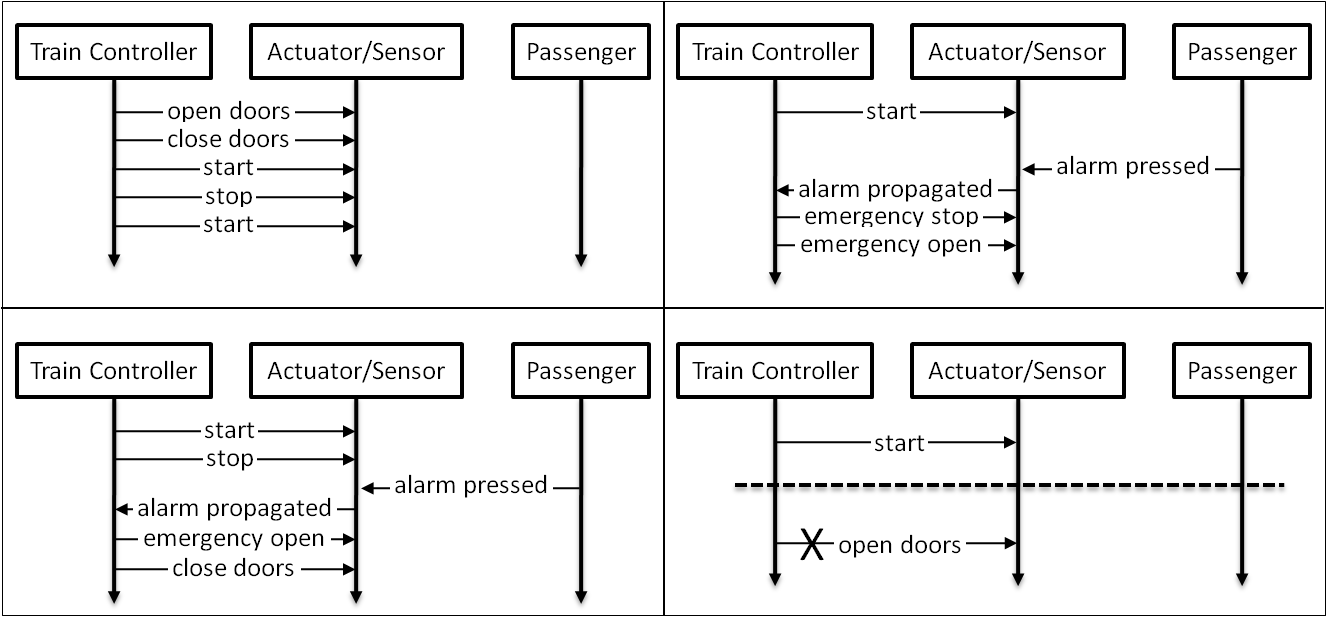
\includegraphics[trim=3mm 3mm 3mm 3mm, clip]{src/4-inductive/images/four-initial-scenarios}}
\caption{Initial positive and negative scenarios for a train system\label{Fig:init:scen}.}
\end{figure}


\item[ChooseStatePair] The candidate solution is refined by merging well- selected state pairs. The \texttt{ChooseStatePair} function determines which pairs to consider. It relies on the standard order $<$ on strings. Each state of the PTA can be labeled by its unique prefix from the initial state. Since prefixes can be sorted according to that order, the states can be ranked accordingly. For example, the PTA states in Fig.~\ref{Fig:algo:steps} are labeled by their rank according to this order. The algorithm considers states $q$ of the PTA in increasing order. The state pairs considered for merging only involve such state $q$ and any state $q'$ of lower rank. The $q'$ states are considered in increasing order as well. This particular ordering is specific to the original RPNI algorithm.

\item[Merge] The \texttt{Merge} function merges the two states $(q, q')$ selected in order to compute a quotient automaton, that is, to generalize the current set of positive behaviors. In the example of Fig.~\ref{Fig:algo:steps}, we assume that states 0, 1, and 2 were previously determined not to be compatible for merging (through negative scenarios initially submitted or generated scenarios that were rejected by the user). Merging a candidate state pair may produce a non-deterministic LTS. For example, after having merged $q = 3$ and $q' = 0$ in the upper part of Fig.~\ref{Fig:algo:steps}, two transitions labeled \texttt{start} from state 0 lead to states 2 and 6, respectively. In such a case, the \texttt{Merge} function merges states 2 and 6 and, recursively, any further pair of states that introduces non-determinism. 

We call \textsl{merging for determinization} this recursive operation of removing non-determinism. This operation guarantees that the current solution at any step is deterministic. It produces an automaton which may accept a more general language than the one it starts from. Therefore, it is not equivalent to the standard algorithm to transform a non deterministic automaton into a deterministic one accepting the same language~\cite{Hopcroft:1979}. Notably, the time complexity of merging for determinization is a linear function of the number of states of the automaton it starts from whereas the standard determinization algorithm is exponential in the worst case. Also, the resulting automaton is still part of the same inductive search space (see Section~\ref{subsection:gi-background-search-space}). 

\begin{figure}
\centering
\scalebox{.67}{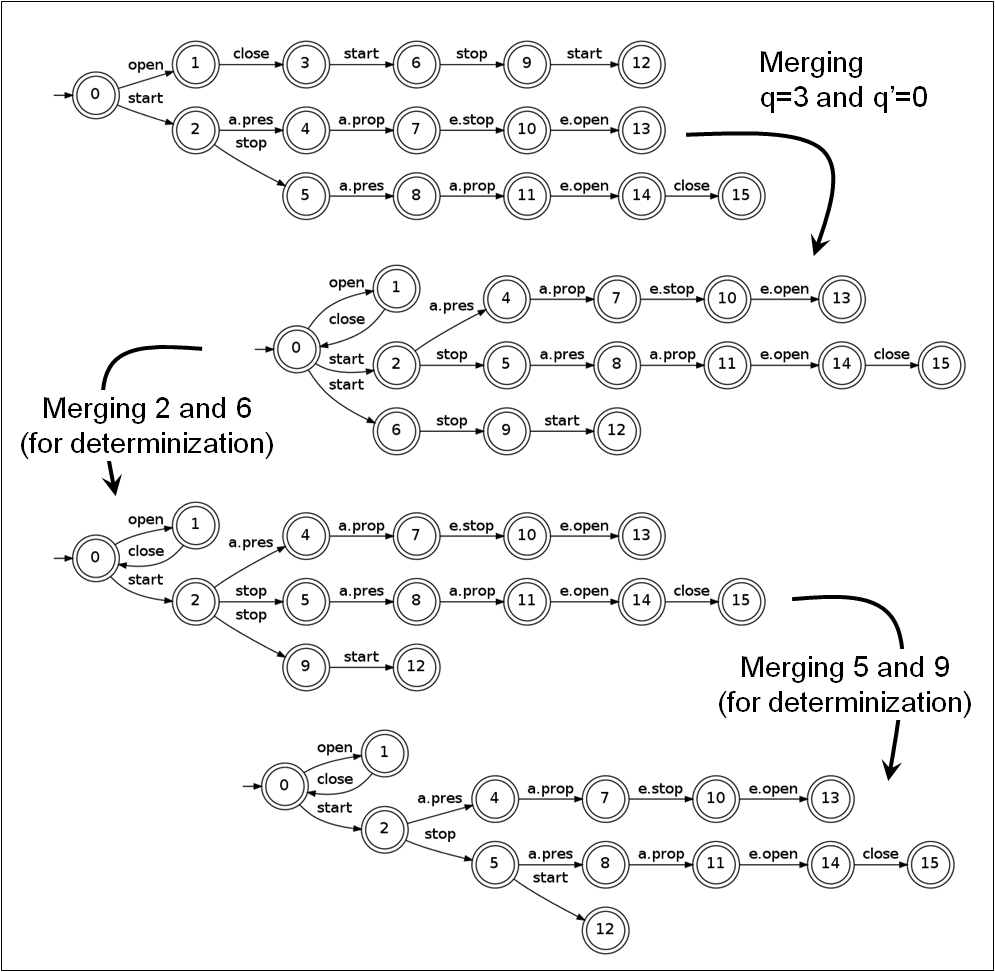
\includegraphics[trim=3mm 3mm 3mm 3mm, clip]{src/4-inductive/images/algo-steps}}
\caption{A typical induction step of the \textsc{QSM} algorithm\label{Fig:algo:steps}.}
\end{figure}

When two states are merged, the rank of the resulting state is defined as the lowest rank of the pair; in particular, the rank of the merged state when merging $q$ and $q'$ is defined as the rank of $q'$ by construction. If no compatible merging can be found between $q$ and any of its predecessor states according to $<$, state $q$ is said to be \textsl{consolidated}. In the example, states 0, 1, and 2 are consolidated.

\item[Consistent] The \texttt{Consistent} function checks whether the automaton $A_{new}$ correctly rejects all negative scenarios. As seen in the pseudo code, the quotient automaton is discarded by \textsc{QSM} when it is detected not to be consistent.

\end{description}

\subsection{Generating queries submitted to the end-user\label{QSM:query}}

This section describes how queries are generated in the \textsc{QSM} algorithm and how the answers provided by the end-user are processed.

\begin{description}

\item[GenerateQuery] When an intermediate solution is consistent with the available scenarios, new scenarios are generated for classification by the end-user as positive or negative. The aim is to avoid poor generalizations by enriching the possibly limited collection of initial scenarios. The notion of characteristic sample drives the identification of which new scenarios should be generated as queries. 

Recall from section~\ref{subsection:gi-background-rpni} that a sample is characteristic of a regular language $L$ if it contains enough positive and negative information. On the one hand, the required positive information is the set of short prefixes $Sp(L)$ which form the shortest histories leading to each state of the canonical automaton $A(L)$. This positive information must also include all elements of the kernel $N(L)$ which represents all system transitions, that is, all shortest histories followed by any admissible event. If such positive information is available, $A(L)$ can always be derived from the PTA by an appropriate set of merging operations. On the other hand, the negative traces provide the necessary information to make incompatible the merging of states which should be kept distinct. A negative trace which would exclude the merging of a state pair $(q, q')$ can be simply made of the shortest history leading to $q'$ followed by any continuation from state $q$ as detailed below.

Consider the current solution of our induction algorithm when a pair of states $(q, q')$ is selected for merging (line 5 in the pseudo code). By construction, $q'$ is always a consolidated state at this step of the algorithm; that is, $q'$ is considered to be in $Sp(L)$. State $q$ is always both the root of a tree and the child of a consolidated state. In other words, $q$ is situated at one letter of a consolidated state, that is, $q$ is considered to be in $N(L)$. States $q$ and $q'$ are compatible according to the available negative scenarios; they would be merged by the standard RPNI algorithm. The QSM extension will first confirm or infirm the compatibility of $q$ and $q'$ by generating scenarios to be classified by the end-user. The generated scenarios are constructed as follows.

\begin{figure}
\centering
\scalebox{.75}{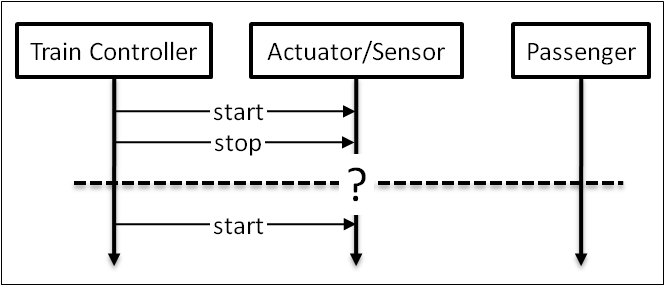
\includegraphics[trim=3mm 3mm 3mm 3mm, clip]{src/4-inductive/images/scenario-question}}
\caption{A new scenario to be classified by the end-user\label{Fig:generated:question}.}
\end{figure}

Let $A$ denote the current solution, $L(A)$ the language generated by $A$, and $A_{new}$ the quotient automaton computed by the \texttt{Merge} function at some given step. Let $x \in Sp(L)$ and $y \in N(L)$ denote the short prefixes of $q'$ and $q$ in A, respectively. Let $u \in L(A)/y$ denote a suffix of $q$ in $A$. 

A generated scenario is built from a system trace $xu$ such that $xu \in L(A_{new})\setminus L(A)$; it can be further decomposed as $xvw$ such that $xv \in L(A)$. The trace $xu$ is thus constructed as the short prefix of $q'$ concatenated with a suffix of $q$ in the current solution, provided the entire behavior is not yet accepted by $A$. Such system trace can be converted to MSC using the structural information provided by a context diagram \cite{Jackson:1995}. The scenario is made of two parts: the first part $xv$ is an already accepted behavior whereas the second part $w$ provides a continuation to be checked for acceptance by the end-user. When submitted to the end-user, the generated scenario can always be rephrased as a question: after having executed the first episode ($xv$), can the system continue with the second episode ($w$)? 

Consider the example in Fig.~\ref{Fig:algo:steps} with selected state pair $q=3, q'=0$. As $q'$ is the root of the PTA, its short prefix is the empty trace $\lambda$. The suffixes of $q$ here yield one generated question (Fig.~\ref{Fig:generated:question}), which can be rephrased as follows: when having started and stopped the train, can the controller restart it? One can see that the first episode of this scenario in Fig.~\ref{Fig:algo:steps} is already accepted by $A$ whereas the entire behavior is accepted in $A_{new}$.

\item[CheckWithEndUser] When a new scenario is generated, it is submitted as a query to the end-user. If the end-user classifies the $Query$ as positive, it is added to the collection of positive scenarios. This addition changes the search space as it extends $S^+$ and consequently the PTA. However, this extension is implicit as the new solution $A_{new}$ is, by construction, also a quotient automaton of this extended PTA. When the $Query$ is classified as negative the induction process is recursively started on the extended scenario collection.

\end{description}

The QSM algorithm has a polynomial time complexity in the size of the learning sample $\mathcal{L}^+(Sc)$, see \cite{Dupont:2008}. 

Moreover, when it receives a characteristic sample in the initial scenario collection it is guaranteed that no additional scenario can be classified as negative. It follows that QSM will not be called recursively anymore and stops by returning the target model. 

An experimental study of the actual sample size required to observe the convergence of \textsc{QSM} and the number of queries submitted to the end-user is detailed in Chapter~\ref{chapter:evaluation}.

\subsection{Reducing the number of queries; the blue-fringe optimization\label{BlueFringe}}

The order in which states are considered for merging by the \texttt{ChooseStatePair} function described in section~\ref{QSM:merging} follows from the implicit assumption that the current sample is characteristic. Consequently, two states are considered compatible for merging if there is no suffix to distinguish among them. This can lead to a significant number of scenarios being generated to the end-user when the initial sample is sparse and actually not characteristic for the target System LTS. 

To overcome this problem, one can use an optimized strategy known as Blue-Fringe~\cite{Lang:1998}. The difference lies in the way state pairs are considered for merging. The general idea is to early detect incompatible state pairs and, subsequently, first consider state pairs for which compatibility has the highest chance to be confirmed by the user through positive classification. The resulting ``please confirm'' interaction may also appear more appealing to the user.

\begin{figure}
\centering
\scalebox{.55}{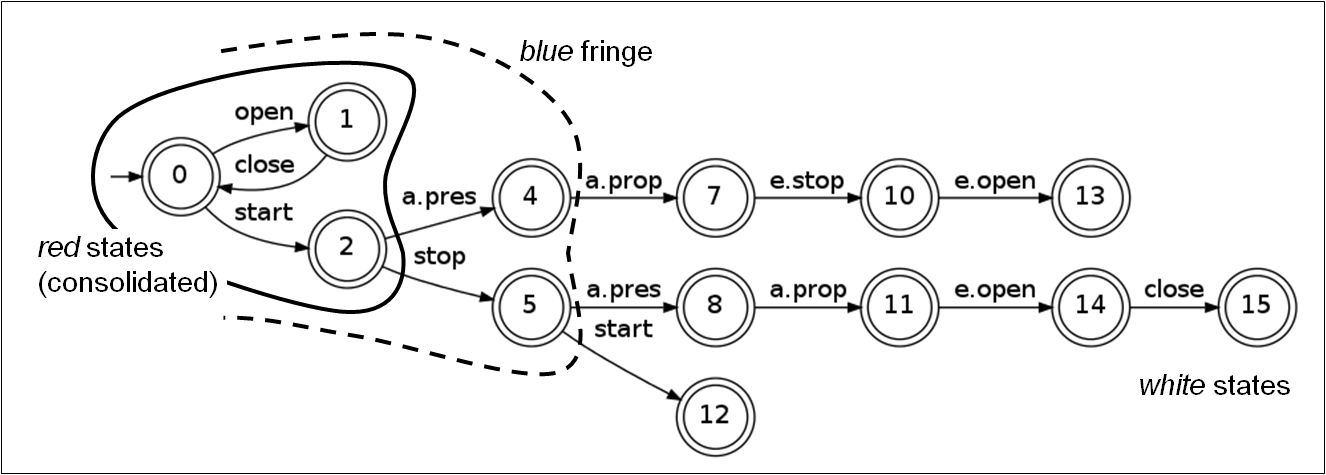
\includegraphics[trim=3mm 3mm 3mm 3mm, clip]{src/4-inductive/images/blue-fringe}}
\caption{Consolidated states (red) and states on the fringe (blue) in a temporary solution\label{Fig:BlueFringe}.}
\end{figure}

Fig.~\ref{Fig:BlueFringe} gives a typical example of a temporary solution produced by the original algorithm. Three state classes can be distinguished in this LTS. The red states are the consolidated ones (0, 1 and 2 in this example). Outgoing transitions from red states lead to blue states unless the latter have already been labeled as red. Blue states form the blue fringe (4 and 5 in this case). All other states are white states. 

The original \texttt{ChooseStatePair} function described in section~\ref{QSM:merging} considers the lowest-rank blue state first (state 4 here) for merge with the lowest-rank red state (0). When this choice leads to a compatible quotient automaton, generated scenarios are submitted to the end-user; in this case, a scenario equivalent to the trace \artifact{<alarm propagated, emergency stop, emergency open>}. The above strategy may lead to multiple queries being generated to avoid poor generalization. Moreover, such queries may be non-intuitive for the user, \textit{e.g.} the \artifact{alarm propagated} event is sent to the train controller without having been fired by the \artifact{alarm pressed} event to the sensor.

To select a state pair for merging, the Blue-Fringe strategy evaluates all (red, blue) state pairs first. The \texttt{ChooseStatePair} function now calls the \texttt{Merge} and \texttt{Compatible} functions before selecting the next state pair. If a blue state is found to be incompatible with all current red states, it is immediately promoted to red; the blue fringe is updated accordingly and the process of evaluating all (red, blue) pairs is iterated. When no blue state is found to be incompatible with red states, the most compatible (red, blue) pair is selected for merging. This is dictated by a scoring mechanism implemented in the \texttt{Compatible} function (see below).

For implementing the Blue-Fringe strategy, it is convenient to adapt \texttt{Initialize} so as to build an \emph{augmented} prefix tree acceptor. Such PTA captures the negative traces in $\mathcal{L}^-(Sc)$ in addition to the positive traces in $\mathcal{L}^+(Sc)$. States reached by a negative trace are tagged as error states; they are depicted in black, as in Fig. \ref{figure:augmented-pta}. 

The \texttt{Compatible} function is also updated to return a compatibility score instead of a boolean value. The score is defined as $-\infty$ when merging the current (red, blue) pair leads to merge an accepting state and an error state during merging for determinization\footnote{in the case of a prefix-closed language, non-error states are all accepting. Recall that this is not necessarily true for any regular language.}; this score indicates an incompatible merging. Otherwise, the compatibility score measures how many accepting states have been merged together. The (red, blue) pair with the highest compatibility score is considered first. The strategy can be further refined with a compatibility threshold $\alpha$ as additional input parameter. Two states are considered to be compatible if their compatibility score is above that threshold. This additional parameter controls the level of generalization since increasing $\alpha$ decreases the number of state pairs that are considered compatible for merging; it thus decreases the number of generated queries.

\begin{figure}\centering
\scalebox{.35}{\includegraphics*{src/4-inductive/images/augmented-pta}}
\caption{Augmented PTA for scenarios in Fig.~\ref{Fig:init:scen}\label{figure:augmented-pta}.}
\end{figure}

Experimental results about the effectiveness of using QSM with and without the Blue-Fringe strategy are detailed in Chapter~\ref{chapter:evaluation}.

\section{Using constraints for multi-view consistency\label{section:inductive-mutliview-consistency}}

The interactive QSM algorithm described in Section~\ref{section:lts-induction-from-mscs} provides a system LTS consistent with all available positive and negative scenarios. The Blue-Fringe strategy can also be applied to reduce the number of additional scenarios submitted to the end-user. The latter strategy relies on two equivalence classes partitioning the states of an augmented PTA. These classes correspond to the accepting states and the error states, respectively. All states belonging to the same class are not necessarily merged in the final solution; however, the \texttt{Compatible} function guarantees that only states belonging to the same class \emph{can} be merged.

This approach can be extended to achieve multi-view consistency by incorporating various sources of information. Such information refines the equivalence partition and further constrains the compatible merging operations. Injecting knowledge-based constraints has many advantages: 
\begin{itemize}
\item It ensures strong consistency of the system LTS with other views;
\item It reduces the number of scenario queries in the interactive setting;
\item It speeds up the search.
\end{itemize}

Section \ref{subsection:induction-pruning-with-domain-knowledge} shows how to incorporate domain knowledge such as fluent definitions. Section \ref{subsection:induction-pruning-with-goals} shows how goals can be used to constrain the generalization. 

The optimization techniques detailed hereafter are based on various equivalence relations over system states. The term \emph{equivalence relation} is used here in its usual mathematical sense, namely, a symmetric, reflexive, and transitive binary relation over states. The general principle underlying our techniques is the following:
\begin{quote}
\emph{Two states will be considered for merging if they agree according to all considered equivalence relations.}
\end{quote}

%%%%%

\subsection{Injecting domain knowledge\label{subsection:induction-pruning-with-domain-knowledge}}

The domain knowledge used to constrain state merging comes from multiple sources: 
\begin{itemize}
\item Fluent definitions;
\item Knowledge about components in the environment of the software-to-be;
\item Specifications of domain properties.
\end{itemize}
We discuss them successively.

%%

\subsubsection*{Propagating fluents}

Fluent definitions provide simple and easy-to-provide domain descriptions to constrain induction. For example, the definition
\begin{center}
fluent $DoorsClosed = \textless \{$close doors$\}, \newline
 \{$open doors, emergency open$\} \textgreater $ initially $true$ \\
\end{center}
describes train door states as being either closed ($DoorsClosed = true$) or open ($DoorsClosed = false$); it also states which event is responsible for which state change. 

Such descriptions can be effectively used to constrain the induction process so that the synthesized System LTS conforms to them. The idea is to decorate each state of the PTA with the value of every fluent. This can be done using a symbolic execution algorithm \cite{Damas:2006, Damas:2011} (see Section~\ref{section:background-fluents}).

The pruning rule for constraining the induction process is here to \emph{avoid merging inconsistent states} according to these decorations. 

The specific equivalence relation is thus the set of state pairs where both states have the same fluent value assignment. The decoration of the merged state is simply inherited from the states being merged.
\begin{quote}
\emph{Two states will be considered for merging if they have the same value for every fluent.}
\end{quote}

Fig.~\ref{dc-augmented-pta} shows the result of propagating the values of the fluent \emph{DoorsClosed} along the augmented PTA built from the scenarios described in Fig.~\ref{Fig:init:scen}.

\begin{figure}
\centering
\scalebox{.33}{\includegraphics*{src/4-inductive/images/dc-augmented-pta}}
\caption{Propagating fluents along the PTA to prune the inductive search space\label{dc-augmented-pta} (DC stands for \emph{DoorsClosed})}
\end{figure}

%%

\subsubsection*{Unfolding models of external components}

Quite often the components being modeled need to interact with other components in their environment - \textit{e.g.}, legacy components in a bigger existing system, foreign components in an open system, etc. In such cases the behavior of external components is generally known - typically, through some behavioral model \cite{Hall:2004}. External components are assumed here to be known by their LTS model. 

For example, Fig.~\ref{Fig.:alarm-sensor} shows the LTS for a legacy alarm sensor in our train system. When the alarm button is pressed by a passenger, this component propagates a corresponding signal to the train controller. 

\begin{figure}
\centering
\scalebox{.4}{\includegraphics*{src/4-inductive/images/alarm-sensor}}
\caption{LTS model for an alarm sensor\label{Fig.:alarm-sensor}.}
\end{figure}

A LTS model of an external component can constrain the induction process so that the synthesized system LTS conforms to it. The idea is to decorate the PTA with states of the external LTS by unfolding the latter onto the PTA. Such decoration is performed by jointly visiting the PTA and the external LTS; the latter synchronizes on shared events and remains in its current state on other events.

Fig.~\ref{Fig.:alarm-unfolded-pta} shows the result of unfolding the alarm sensor LTS from Fig.~\ref{Fig.:alarm-sensor} on the augmented PTA built from the scenarios described in Fig.~\ref{Fig:init:scen}. Each state of the PTA is labeled with the number of the corresponding state in the alarm sensor LTS. 

\begin{figure}
\centering
\scalebox{.35}{\includegraphics*{src/4-inductive/images/alarm-unfolded-pta}}
\caption{Unfolding the alarm sensor LTS onto the PTA\label{Fig.:alarm-unfolded-pta}.}
\end{figure}

The pruning rule for constraining the induction process is now to \emph{avoid merging states decorated with distinct states of the external component}. The specific equivalence relation used here is the set of states where both states have the same external LTS state. 

\begin{quote}
\emph{Two states will be considered for merging if they have the same external LTS state.}
\end{quote}

%%

\subsubsection*{Using declarative domain properties}

Descriptive statements and assumptions about the domain can be expressed declaratively in FLTL (see Section~\ref{section:background-goals}). For example, the physical law
\begin{align*}
\square(HighSpeed \rightarrow Moving)
\end{align*}
\noindent excludes all negative traces where the train is running at high speed while not moving. 

The technique for constraining induction through descriptive or prescriptive statements is the same; we discuss it hereafter.

%%%%%

\subsection{Injecting goals\label{subsection:induction-pruning-with-goals}}

For reasons discussed in Section \ref{section:background-goals}, we restrict our attention to goals and domain properties that can be formalized as pure FLTL safety properties. Remember that these properties refer to  ``\emph{something bad may never happen}''.

Consider the following goal requiring train doors to remain closed while the train is moving:
\begin{center}
\artifact{Maintain[DoorsClosed While Moving]} = $\square(Moving \rightarrow DoorsClosed)$
\end{center}

Fig.~\ref{Fig.:tester-automaton-inductive} shows the tester automaton for this property (cfr. Section \ref{subsection:background-property-and-tester-automata}). The accepting state of this tester captures all traces violating the safety property; any trace leading to it corresponds to an undesired system behavior. In particular, the trace \artifact{<start, open>} corresponds to the initial negative scenario in Fig.~\ref{Fig:init:scen}. As seen in Fig.~\ref{Fig.:tester-automaton-inductive}, the tester provides many more negative traces. Property testers can in fact provide potentially infinite classes of negative scenarios.

\begin{figure}
\centering
\scalebox{.35}{\includegraphics*{src/4-inductive/images/tester-automaton}}
\caption{Tester LTS for the goal \artifact{Maintain[DoorsClosed While Moving]}.\label{Fig.:tester-automaton-inductive}}
\end{figure}

The property tester is used to constrain the induction process in a way similar to an external component LTS. The PTA and the tester are traversed jointly in order to decorate each PTA state with the corresponding tester state. Fig.~\ref{Fig.:goal-unfolded-pta} shows the PTA decorated using the tester of Fig.~\ref{Fig.:tester-automaton-inductive}.

\begin{figure}
\centering
\scalebox{.35}{\includegraphics*{src/4-inductive/images/goal-unfolded-pta}}
\caption{Augmented PTA decorated using the tester automaton from Fig.~\ref{Fig.:tester-automaton-inductive}\label{Fig.:goal-unfolded-pta}.}
\end{figure}

The pruning rule for constraining the induction process is now to \emph{avoid merging states decorated with distinct states of the property tester}. The specific equivalence relation used here is the set of states where both states correspond to the same state of the property tester. 
\begin{quote}
\emph{Two states will be considered for merging if they have the same property tester state.}
\end{quote}

This pruning technique guarantees the consistency between the synthesized System LTS and the considered goals and domain properties. In other words, for every goal or domain property $G$ injected in the synthesis process, the following consistency condition holds (see Section \ref{subsection:background-goals-consistency}):
\begin{align*}
\mathcal{L}^-(G) \cap \mathcal{L}(System) &= \emptyset,
\end{align*}
where \emph{System} here denotes the synthesized system LTS and $\mathcal{L}^-(G)$ captures all traces violating $G$.

Note that the guarantee given by the above condition is weaker than the \emph{consistent system view} condition (\ref{relation:inductive-statement-negative}) in Section \ref{subsection:inductive-synthesis-statement}. The latter requires the consistency of the synthesized system $\system$ while the above condition only applies to the system LTS. As with implied negative scenarios, a goal could be satisfied by the synthesized System LTS while being violated by the real distributed system. This issue is further discussed in Section \ref{section:inductive-discussion}.

\subsection{Discussion\label{subsection:qsm-constraints-implementation-notes}}

The equivalence relations considered in the previous sections are all invariant under state merging. In other words, a state derived by merging some states simply inherits their relation. This allows each relation to be computed only once on the initial PTA; the results of such pre-processing are kept as annotations on PTA states. 

Our implementation reuses the decoration algorithm from \cite{Damas:2006} to propagate fluent values on the PTA (see Section~\ref{subsection:fluents-along-multiple-traces}). Its generalization in~\cite{Damas:2011} may be used as an effective mean to unfold models of legacy components and tester automata on the PTA without additional developments.

The principle for constraining state merging through equivalence relations first appeared in~\cite{Coste:1998, Coste:2004}. It can be further instantiated to other equivalence relations not considered here. In particular, it is \emph{not} limited to relations that are invariant under state merging.

As an illustrative example, consider the following generalization of the way fluent values are used to constrain the induction process. We know from Section~\ref{subsection:fluents-along-multiple-traces} that the states of any LTS can be annotated with invariants defined on fluents. Let $inv$ denote the function mapping each PTA state to its state invariant; let also denote by \emph{Dom} a domain property that must be met in every state of the system LTS. Consider the following pruning rule:
\begin{quote}
\emph{Two states $q$ and $q'$ will be considered for merging if $inv(q) \wedge inv(q') \models \mbox{Dom}$}
\end{quote}

The equivalence relation here is the set of state pairs whose conjunction of invariants satisfies the domain property. This equivalence relation is \emph{not} invariant under state merging. The merging constraint can however be enforced; to achieve this, the compound state resulting from merging $q$ and $q'$ has to be annotated by the conjunction of their state invariants; this new invariant is then used in subsequent state merging.

In the general case of DFA induction\footnote{that is, in contrast to LTS induction}, a similar mechanism is needed to implement the Blue-fringe optimization with an augmented PTA. In that case, an error state may be merged with a non accepting state provided the result is not merged later with an accepting one. That is, the relation capturing the equivalence of states in terms of their continations is not invariant under state merging.

\section{LTS synthesis from high-level MSCs\label{section:inductive-from-hMSC}}

The previous sections have shown how system behaviors specified in collections of MSC scenarios can be first generalized as a System LTS, then decomposed as a set of agent LTSs. The technique supports the incremental enrichment of an initial scenario collection through scenario queries. It also takes other models into account, such as goals, so as to preserve multi-view consistency. Behavior generalization, incremental synthesis and multi-view consistency are the three main requirements identified in Section \ref{subsection:inductive-synthesis-requirements}. 

Coupled with other synthesis techniques such as goal mining from scenarios\footnote{whose simplest form consists in asking ``why'' when facing with a negative scenario.} \cite{Damas:2006}, interactive LTS induction is really effective; starting from a small initial scenario collection, richer system models can be synthesized in only a few iterations. Chapters~\ref{chapter:evaluation} and \ref{chapter:tool-support} illustrate this claim with evaluations and overview of the tool support.

However, for any non-toy system, a large scenario collection might become unmanageable. Among others, consistency of the collection might be difficult to guarantee without costly refactoring on scenarios. One reason is that all scenarios of a collection are required to start in the same system state; this usually implies a lot of redundancy in system descriptions.

One way to tackle this problem is to use high-level message sequence charts (hMSCs) for structuring scenario descriptions. As detailed in Section \ref{subsection:background-hmsc}, hMSCs are directed graphs where each node refers to a MSC or a finer grained hMSC (see Fig.~\ref{image:train-hmsc}). Scenarios can then be structured by introducing alternatives, sequences and loops.

Having a structured form of scenario \emph{helps} specifying a large system with scenarios; it does not \emph{solves} the problem of achieving a complete and consistent view of agent behaviors:
\begin{itemize}
\item capturing all possible interleavings of a distributed system proves difficult with scenarios; a hMSC is therefore hardly complete in practice,
\item complementary features of a system deserve being specified in complementary models; in addition to using multiple system views, having system behaviors specified in more than one hMSC makes sense.
\end{itemize}

Having a synthesis technique to merge and to generalize behaviors described in hMSCs seems a convenient extension to the synthesis technique described so far. For this, the LTS synthesis statement is first revisited in Section~\ref{subsection:hmsc-induction-problem-revisited}. The inductive algorithm is then adapted in Section \ref{subsection:hmsc-induction-algo-adaptation}.

\subsection{Revisiting the LTS synthesis statement\label{subsection:hmsc-induction-problem-revisited}}

Merging multiple hMSCs $H_1,\ldots,H_n$ with respect to trace behaviors simply amounts to compute the union of their respective languages. This is equivalent to building a new hMSC $H$ reaching the finer-grained $H_1,\ldots,H_n$ from its initial state. Additional positive scenarios $S^+_1,\ldots,S^+_n$, typically coming from scenario queries, could be integrated in a similar way. This is illustrated in Fig.~\ref{figure:multiple-hmscs}.

\begin{figure}\centering
\scalebox{.70}{
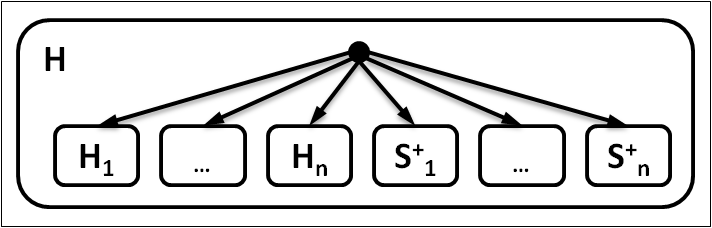
\includegraphics[trim=3mm 3mm 3mm 3mm, clip]{src/4-inductive/images/multiple-hmscs}}
\caption{Merging multiple hMSCs amounts to builds a new one that reaches finer-grained hMSCs from its initial state.\label{figure:multiple-hmscs}} 
\end{figure}

However, a hMSC only permits specifying positive behaviors. As explained in previous sections, negative information is needed to avoid poor generalizations. Negative scenarios, fluents, goals, etc. all provide a source of negative knowledge that can be used to constraint the induction process. The algorithmic adaptations considered later stay compatible with the constraint mechanism based on equivalence relations on system states.

Without loss of generality therefore, we will assume that behaviors are specified through one hMSC only, complemented with a scenario collection. The latter contains negative scenarios and answers to scenario queries. Under these assumptions, the LTS synthesis statement is restated as follows: 

\begin{quote}
\underline{Given}~a hMSC $H$ and a scenario collection $Sc = (S^+,S^-)$ consistent with each other
\begin{align*}
[\mathcal{L}^+(Sc) \cup \mathcal{L}(H)] \cap \mathcal{L}^-(Sc) &= \emptyset
\end{align*}
\underline{Synthesize}~the system as a composition of agent LTSs
\begin{align*}
System = (Ag_1 \parallel \ldots \parallel Ag_n)
\end{align*}
\underline{Such that}~$H$, $Sc$ and $System$ are consistent.
\end{quote}

The hMSC trace semantics is left open in the formulation above. In other words, one has to decide which set of behaviors does $\mathcal{L}(H)$ denote. We recall below the relations between the three hMSC languages covered in Section \ref{subsection:background-hmsc}: 
\begin{align}
\mathcal{L}_{strong}(H) \subseteq \mathcal{L}_{weak}(H) &\subseteq \mathcal{L}_{arch}(H)
\end{align}

$\mathcal{L}_{strong}(H)$ denotes the set of system behaviors with strong sequential composition of hMSC nodes and total event ordering inside MSCs. It is the simplest and most intuitive model for stakeholders involved in early phases of system design. However, it supposes an implicit synchronization scheme used by the agents that is usually not available in real distributed systems. $\mathcal{L}_{arch}(H)$ is the most realistic for such systems, as it captures all possible interleavings of agent behaviors. $\mathcal{L}_{weak}(H)$ is mainly used for explaining and detecting implied scenarios in hMSC specifications \cite{Uchitel:2003}; it is also the hardest to compute.

Making a choice of semantics is required for generalizing behaviors because inductive synthesis takes a set of traces as input. The chosen semantics must of course fit domain assumptions. From an algorithmic point of view however, the three hMSC languages above require the same adaptations of the inductive process, as explained in the next sections.

\subsection{Generalizing high-level MSC languages\label{subsection:hmsc-induction-algo-adaptation}}

Recall that learning a regular language $L$ aims at generalizing a positive sample $S_+$ under the control of a negative sample $S_-$ such that the following relation of language inclusions holds:
\begin{align}
S_+~~\subseteq~~L~~\subseteq~~\Sigma^*\setminus S_-
\end{align}

LTS synthesis from a scenario collection $Sc$ reduces to grammar induction because the sets $\mathcal{L}^+(Sc)$ and $\mathcal{L}^-(Sc)$ are valid positive and negative samples, respectively (see Section \ref{subsection:inductive-lts-synthesis-reduction}). In particular, they denote \emph{finite} sets of traces.

When considering the generalization of hMSC behaviors, the sets of positive and negative traces are $\mathcal{L}^+(Sc) \cup \mathcal{L}(H)$ and $\mathcal{L}^-(Sc)$, respectively. The positive set is no longer a sample because $\mathcal{L}(H)$ might contain an infinite number of traces. Therefore, the current problem statement no longer fits exactly in the identification in the limit framework presented in Section \ref{section:inductive-background}. 

From a theoretical point of view, it means that generalizing hMSC languages is a different problem than generalizing MSC languages; therefore, further study would be needed to re-state the convergence criteria and the notion of characteristic sample in particular. From an algorithmic point of view, however, only a few adaptations of RPNI and QSM are required. They are explained in the next section.

\subsection{The Automaton State Merging algorithm\label{subsection:automaton-state-merging}}

The algorithm to generalize behaviors specified in a hMSC is given in Algorithm~\ref{ASM}, called Automaton State Merging (ASM). It is very similar to QSM, given in Section~\ref{section:lts-induction-from-mscs}, except that the interactive feature is ommited here (we discuss it later). QSM itself being an interactive extension to RPNI, Algorithm~\ref{ASM} is almost RPNI itself which might appear suprising at first glance.

\begin{algorithm}
{
\vspace{0.2cm}
\KwIn{A high-level MSC $H$ and a scenario collection $Sc = (S_+, S_-)$}
\KwOut{A System LTS, consistent with both $H$ and $Sc$}

$A \leftarrow $ {\tt Initialize($H$, $Sc$)}\\
\While{$(q,q') \leftarrow $ {\tt ChooseStatePair($A$)}}{
$A_{new} \leftarrow$ {\tt Merge$(A,q,q')$}\\
\If{{\tt Consistent$(A_{new}, S_-)$}}{
 $A \leftarrow A_{new}$
}
}
\Return{$A$}}
\vspace{0.2cm}
\caption{\textsc{ASM}, a state-merging algorithm from high-level Message Sequence Charts\label{ASM}}
\end{algorithm}

The main difference between RPNI and QSM on one side and ASM on the other side is the initial automaton solution built by \texttt{Initialize}. RPNI and QSM initially convert the input \emph{sample} as a PTA, hence a tree, whereas ASM converts the input \emph{language} of the hMSC as a DFA, hence an graph. The main loop of the ASM algorithm can then be seen as generalizing any regular language, under the control of a negative sample; hence the ``Automaton State Merging'' name. A few adaptations are however required to the different functions of the algorithm: 

\begin{description}

\item[Initialize] This function is adapted to return a DFA instead of a PTA. On one side, the positive traces from the hMSC may be captured through a LTS as discussed in Section \ref{subsection:background-hmsc}, provided a choice of hMSC semantics. On the other side, the scenario collection can be captured through a PTA. These two automata can be merged through standard algorithms for capturing the union of regular languages \cite{Hopcroft:1979}. 

In order to use the Blue-Fringe heuristic (see below), the obtained DFA may be augmented with error states encoding the negative sample given by $S_-$. 

\item[ChooseStatePair] In order to preserve the merging order used by RPNI, this function must be slightly adapted. The idea is to pre-compute the natural order among the states of the initial DFA solution. A breadth first search is used and each of them is numbered when encountered. 

Not that the Blue-Fringe strategy does not require special support. The distinction between red and blue states does not rely on any assumption about the initial solution being a tree; in particular, the fact that a fringe state is the root of a tree in RPNI and QSM is incidental (see \texttt{Merge} below).

\item[Merge] The merging for determinization process is often implemented assuming a tree invariant property. This property states that, when considering two states to be merged, at least one of them is the root of a tree. Such a property holds for RPNI and QSM, even when the Blue-Fringe optimization is used. It is a sufficient condition for the determinization process to be finite. 

Even though it is convenient, the tree invariant property is not required, as explained in \cite{Lambeau:2008}. The main merging loop and the \texttt{Merge} function can be implemented without the tree invariant property because the recursive determinization process stops naturally on the first DFA encountered. This observation allows one to start from an arbitrary DFA and, as soon as non-determinism occurs, to reduce it. 
%Fig.~\ref{figure:merging-for-determ-on-dfa} gives an example of such a recursive operation.

\end{description}

The interactive feature of QSM could be easily adapted and plugged to ASM. It consist in replaincing the main loop ASM by the one of QSM (see Algorithm~\ref{QSM} in Section~\ref{section:lts-induction-from-mscs}). In the latter, the \texttt{GenerateQuery} function must be adapted as follows:

\begin{description}

\item[GenerateQuery] The generation of scenario queries relies on the tree invariant property mentioned above. When merging a state pair $(q,q')$, a scenario query is built with the shortest trace leading to $q$ concatenated with the suffixes of $q'$. When $q'$ is the root of a tree, generating a finite scenario is straightforward.

If the tree invariant property no longer holds, the \texttt{GenerateQuery} function must be extended with a procedure for extracting finite suffixes from $q'$. This does not introduce any technical issues; for example, pre-computing a spanning tree on the initial DFA would associate finite suffixes to each of its state. However, what forms a ``good'' suffix for convergence and scenario classification by end-users is an open question. As the adapted algorithm no longer fits in the identification in the limit framework, the notion of a characteristic sample would need to be adapted. 

\end{description}

%\begin{figure}\centering
%\scalebox{.34}{
%\includegraphics*{src/4-inductive/images/merging-for-determ-on-dfa}}
%\caption{Recursive determinization process. States \{3\} and \{0\} of an arbitrary DFA are merged, which causes a non-determinism on letter $b$ from state \{0,3\}. The destination states \{2\} and \{4\} are subsequently merged to reduce the non-determinism.\label{figure:merging-for-determ-on-dfa}} 
%\end{figure}

From a grammar induction point of view, the ASM algorithm can be seen as generalizing any positive regular language $\mathcal{L}^+$ under the control of a negative sample $S_-$. As such, RPNI is thus a special case where the positive language forms a sample $S_+$, that is a finite set of strings.

Interrestingly, the constraint mechanism from Section~\ref{section:inductive-mutliview-consistency} to prune the induction search space and guarantee multi-view consistency can still be used with ASM. Indeed, the partitionning of PTA states according to equivalence relations extracted from domain knowledge can be performed on the input DFA returned by \texttt{Initialize}, \emph{mutatis mutandis}. 

In particular, goals and domain properties can still be used to prune the induction search space, as explained in Section~\ref{subsection:induction-pruning-with-goals}. As goals actually capture negative languages through their tester automaton, this amounts to consider yet another generalization of ASM to generalize a positive language $\mathcal{L}^+$ under the control of a negative one $\mathcal{L}^-$. This generalization is called ASM$^*$ and briefly discussed in \cite{Lambeau:2008}.



\section{Correctness\label{section:inductive-correctness}}

Proving the correctness of our synthesis approach amounts to show that the synthesized system is consistent with both the scenarios and all domain knowledge taken in input. We discuss proof arguments for the different algorithm settings, starting with the simplest case of RPNI-based synthesis and gradually integrating features such as scenario questions and injection of domain knowledge.

\begin{figure}\centering
\scalebox{.65}{
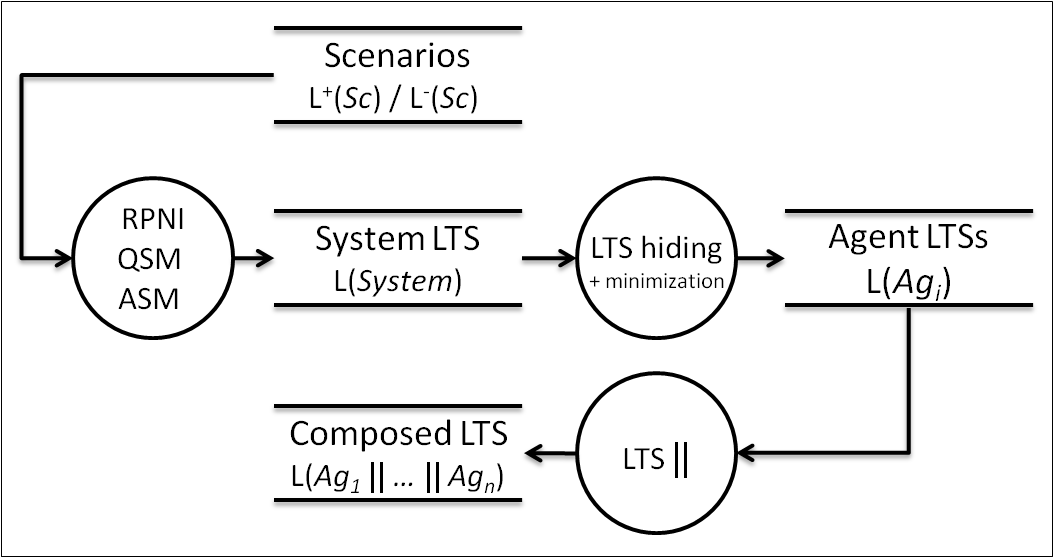
\includegraphics[trim=3mm 3mm 3mm 3mm, clip]{src/4-inductive/images/synthesis-flow-model}}
\caption{Inductive synthesis steps and products.\label{figure:synthesis-flow-model}} 
\end{figure}

Fig.~\ref{figure:synthesis-flow-model} summarizes our approach by showing used algorithms together with their input/output in terms of behavior models and associated languages. 
\begin{itemize}
\item From scenarios, a system LTS is inferred using either RPNI, QSM or ASM. 
\item LTS hiding and minimization is then used to obtain a canonical state machine for each agent. 
\item From the system view point, the result of our synthesis approach is precisely captured by the composition of those state machines.
\end{itemize}

In this figure and in the following discussions,
\begin{itemize}
\item $Sc = (S^+,S^-)$ denotes the input scenario collection; its positive and negative languages are denoted by $\mathcal{L}^+(Sc)$ and $\mathcal{L}^-(Sc)$, respectively.
\item $\mathcal{L}(\me{System})$ denotes the language captured by the inferred system LTS.
\item $\mathcal{L}(Ag)$ denotes the language of an arbitrary agent $Ag$, as captured by its LTS state machine.
\item $\mathcal{L}(\agentscomposed)$ denotes the language captured by the LTS resulting of the composition of individual agent LTSs.
\end{itemize}

We first restrict our attention to the simplest, non-interactive, RPNI approach. Remember from Section~\ref{subsection:inductive-synthesis-statement} that the specification on our approach requires three conditions to hold on synthesized state machines:
\begin{itemize}
\item The \emph{structural consistency} condition requires input scenarios and synthesized agent state machines to agree on the respective agent interfaces.
\item The \emph{consistent agent view} condition requires each synthesized agent state machine to cover the positive behaviors along the corresponding timeline in the input scenarios.
\begin{align}
\mathcal{L}^+(Sc_{\downarrow Ag}) \subseteq \mathcal{L}(Ag)\mbox{~for each agent $Ag$}\label{proof:consistent-agent-view}
\end{align}
where $Sc_{\downarrow Ag}$ denotes the positive behaviors along $Ag$'s timeline in a scenario collection $Sc = (S^+, S^-)$:
\begin{align}
\mathcal{L}^+(Sc_{\downarrow Ag}) = \bigcup_{P \in S^+} \mathcal{L}(P_{\downarrow Ag})~~\cup~~\bigcup_{N \in S^{-}} \mathcal{L}^{+}(N_{\downarrow Ag})\label{proof:lemma-sc-projection}
\end{align}

This is a a slight generalization of the concept of agent traces along a single scenario timeline $M_{\downarrow Ag}$, introduced in Section~\ref{section:background-scenarios}. Observe that it takes both positive and negative scenarios into account.
\item The \emph{consistent system view} requires the system to cover all positive scenarios and reject all negative ones. 
\begin{align}
&\mathcal{L}^+(Sc) \subseteq \mathcal{L}(\agentscomposed)\label{proof:consistent-system-view-1}\\
&\mathcal{L}^-(Sc) \cap      \mathcal{L}(\agentscomposed) = \emptyset\label{proof:consistent-system-view-2}
\end{align}
\end{itemize}

Section~\ref{subsection:system-lts-consistency} briefly discusses the consistency of the inferred system LTS with the scenarios. This result is then used in Section~\ref{subsection:consistent-agent-view} to show that the decomposition step meets the ``structural consistency'' and the ``consistent agent view'' conditions. The ``consistent system view'' condition is further discussed in Section~\ref{subsection:consistent-system-view}. The discussion is pursued in the presence of scenario questions in Section~\ref{subsection:proof-with-scenario-questions} and with the injection of domain knowledge in Section~\ref{subsection:proof-with-domain-knowledge}. Section~\ref{subsection:correctness-of-asm} closes this section with a discussion about the correctness of ASM.

%%%

\subsection{Consistency of the system LTS\label{subsection:system-lts-consistency}}

This section demonstrates that RPNI yields a system LTS consistent with the input scenario collection. The pseudo code given in Algo.~\ref{QSM} is used, ignoring the scenario questions (lines 5 to 10).

\begin{theorem}
\label{theorem:system-lts-consistency-with-sc}
The system LTS synthesized by RPNI covers all positive scenarios and rejects all negative ones.
\begin{align*}
&\mathcal{L}^+(Sc) \subseteq \mathcal{L}(System)\\
&\mathcal{L}^-(Sc) \cap      \mathcal{L}(System) = \emptyset
\end{align*}

\begin{proof}
This theorem is proven by induction using the following invariant:
\begin{align}
&\mathcal{L}^+(Sc) \subseteq \mathcal{L}(A_i)\label{inv:system-lts-consistency-with-sc-1}\\
&\mathcal{L}^-(Sc) \cap      \mathcal{L}(A_i) = \emptyset\label{inv:system-lts-consistency-with-sc-2}
\end{align}

\begin{description}
\item[Base:] $A_0$ denotes the PTA returned by \emph{Initialize}.

The PTA is the largest DFA accepting the positive language; a precondition states that input scenarios are consistent. Therefore the following conditions hold, entailing the invariant:
\begin{align}
&\mathcal{L}^+(Sc) =    \mathcal{L}(A_0)\\
&\mathcal{L}^-(Sc) \cap \mathcal{L}(A_0) = \emptyset
\end{align}

\item[Inductive step:] $A_i$ is the quotient automaton denoting the current solution at step $i$.

From a solution $A_i$, the next solution $A_{i+1}$ is computed by the \emph{Merge} function (see line 3 in Algo.~\ref{QSM}). The latter computes a quotient automaton. Definition~\ref{definition:quotient-automaton} guarantees that such quotient automaton may only generalize the language of $A_i$. As the condition~(\ref{inv:system-lts-consistency-with-sc-1}) holds for $A_i$, the following condition holds as well:
\begin{align*}
&\mathcal{L}^+(Sc) \subseteq \mathcal{L}(A_i) \subseteq \mathcal{L}(A_{i+1})
\end{align*}

On an other hand, quotient automata are only kept as next solution if consistent with the negative scenarios (see lines 4 and 11). Therefore, the following condition holds when such solution is kept (line 11):
\begin{align*}
&\mathcal{L}^-(Sc) \cap \mathcal{L}(A_{i+1}) = \emptyset
\end{align*}

\end{description}
\end{proof}
\end{theorem}

A detailed proof of the convergence of RPNI towards the canonical target automaton when it receives a characteristic sample can be found in~\cite{Oncina:1993} in the more general case of transducer learning.

%%%

\subsection{Structural consistency and consistent agent view\label{subsection:consistent-agent-view}}

Given the consistency of the system LTS with the positive and negative scenarios, the decomposition step guarantees that the \emph{structural consistency} and the \emph{consistent agent view} both hold.

Structural consistency only requires the LTS hiding step to make use of adequate agent alphabets, as induced from the scenarios themselves or given by a (consistent) structural model. We do not discuss it further. 

For each agent $Ag$, the ``consistent agent view'' condition (\ref{proof:consistent-agent-view}) can be derived from (\ref{proof:consistent-system-view-1}) using the following properties and definitions:
\begin{align}
&\mathcal{L}(X) \subseteq \mathcal{L}(Y) \implies \mathcal{L}(X \setminus I) \subseteq \mathcal{L}(Y \setminus I) \label{proof-agent-consistency-1}\\
&\mathcal{L}^+(Sc_{\downarrow Ag}) = \mathcal{L}^+(Sc \setminus \Sigma_{Ag}^c)\label{proof-agent-consistency-2}\\
&\mathcal{L}(Ag) = \mathcal{L}(System \setminus \Sigma_{Ag}^c)\label{proof-agent-consistency-3}
\end{align}
where $\Sigma_{Ag}^c$ denotes the set of all system events excluding those of $Ag$'s interface.
\begin{itemize}
\item (\ref{proof-agent-consistency-1}) states that behavior inclusion is preserved under LTS hiding; this property follows from material in Section~\ref{subsection:lts-hiding}. 
\item (\ref{proof-agent-consistency-2}) rewrites the left term of (\ref{proof:consistent-agent-view}) in terms of hiding of scenario behaviors\footnote{using an abuse of notation as the hiding operator is defined on LTS, not on scenarios collections.}. It can be derived from (\ref{proof:lemma-sc-projection}) and the definition of $M_{\downarrow Ag}$ (see Section~\ref{subsection:background-positive-scenarios}). 
\item (\ref{proof-agent-consistency-3}) follows from the definition (\ref{definition:decomposition-step}) of decomposition step itself (see Section~\ref{subsection:inductive-synthesis-approach}). 
\end{itemize}

From Theorem~\ref{theorem:system-lts-consistency-with-sc} ensuring the consistency of the system LTS with input scenarios, the following condition is established thanks to (\ref{proof-agent-consistency-1})
\begin{align}
&\mathcal{L}^+(Sc \setminus \Sigma_{Ag}^c) \subseteq \mathcal{L}(System \setminus \Sigma_{Ag}^c)\label{proof:consistent-agent-view-milestone}
\end{align}

The ``consistent agent view'' condition (\ref{proof:consistent-agent-view}) is established by substituing the right terms of (\ref{proof-agent-consistency-2}) and (\ref{proof-agent-consistency-3}) in (\ref{proof:consistent-agent-view-milestone}).

%%%

\subsection{Consistent system view: the problem of implied scenarios\label{subsection:consistent-system-view}}

This section discusses the correctness of the ``consistent system view'' condition. The conditions related to the positive and negative scenarios are discussed in turn.

\begin{theorem}
The synthesized system covers all positive scenarios.
\begin{align*}
&\mathcal{L}^+(Sc) \subseteq \mathcal{L}(\agentscomposed)
\end{align*}

\begin{proof}
This condition results from two main properties of our approach:
\begin{itemize}
\item The synthesized system LTS covers all positive scenario behaviors, as guaranteed by Theorem~\ref{theorem:system-lts-consistency-with-sc}.
\begin{align*}
&\mathcal{L}^+(Sc) \subseteq \mathcal{L}(System)
\end{align*}
\item Projecting the system LTS on agent alphabets and recomposing their LTS afterwards does not restrict behaviors:
\begin{align*}
&\mathcal{L}(\mbox{System}) \subseteq \mathcal{L}(\agentscomposed)
\end{align*}
This latter condition can be derived from the definition of agent languages (\ref{proof-agent-consistency-3}) and properties of LTS hiding and composition operators (see Section~\ref{section:background-state-machines}).
\end{itemize} 

\end{proof}
\end{theorem}

\begin{theorem}
The synthesized system excludes all negatives scenarios.
\begin{align*}
&\mathcal{L}^-(Sc) \cap \mathcal{L}(\agentscomposed) = \emptyset
\end{align*}
\end{theorem}

This theorem would require the composed system to exclude all negative scenarios. Due to the potential presence of implied scenarios, our approach only guarantees the weaker condition given by Theorem~\ref{theorem:system-lts-consistency-with-sc}, namely,
\begin{align*}
&\mathcal{L}^-(Sc) \cap \mathcal{L}(\mbox{System}) = \emptyset
\end{align*}

In other words, the induction algorithm ensures that the system LTS excludes all negative scenarios. This property can however be lost after the decomposition and recomposition steps.

The reason has to be found in the possible occurence of so-called \emph{implied scenarios}. Remember from Section~\ref{subsection:background-hmsc} that implied scenarios may appear when a system is specified globally while implemented component-wise ~\cite{Alur:2000, Uchitel:2004}. In our case, the set of implied scenarios is precisely defined as:
\begin{align*}
\mathcal{L}(\agentscomposed) \setminus \mathcal{L}(\mbox{System})
\end{align*}

When this language is not empty, implied scenarios denote system behaviors that the system LTS does not accept but which are exhibited by the composition of agent LTSs. Implied scenarios appear when, once distributed, the agents lack monitoring abilities to restrict their behavior so as to precisely match the system LTS.

Not all implied scenarios are problematic in practice. In particular, it might happen that all implied scenarios denote desired system behaviors. In that case, the presence of implied scenarios is not problematic and may be seen as the result of a second generalization step due to the decomposition and recomposition of agent LTS. This second generalization step proves useful as it weakens the necessity of having a pure structurally complete scenario collection in the first place.

Negative implied scenarios, that is, counterexamples of desired behaviors, are more problematic. In particular, a behavior trace $t$ could be such that the following conditions hold:
\begin{align}
&t \in \mathcal{L}^-(Sc)\label{implied-1}\\
&t \notin \mathcal{L}(\mbox{System})\label{implied-2}\\
&t \in \mathcal{L}(\agentscomposed)\label{implied-3}
\end{align}
that is, (\ref{implied-1}) $t$ denotes a system behavior explicitly rejected through a negative scenario; it might be a question answered negatively; (\ref{implied-2}) $t$ is correctly rejected by the system LTS; (\ref{implied-3}) $t$ is still be exhibited by the composed system.

In such case, observe the ``consistent system view'' condition is not met as (\ref{proof:consistent-system-view-2}) does not hold. As with other scenario approaches, e.g. \cite{Alur:2000, Uchitel:2004}, our synthesis technique fails to guarantee a consistent system view between scenarios and state machines in presence of negative implied scenarios.

In order to detect such situations, the technique from \cite{Uchitel:2004} could be adapted to enumerate implied scenarios and submit them as additional scenario questions to the user (see Section~\ref{section:related-for-analysis-3}). 

Note that, fixing implied scenario problems requires rethinking the system decomposition into agents and/or refactoring their interfaces. In other words, the root cause of implied scenarios problems has to be found in the structural decomposition of the system, not in the particular technique used to infer state machines from scenarios. 

%%%

\subsection{Correctness in the presence of scenario questions\label{subsection:proof-with-scenario-questions}}

The specification of QSM has been strengthened in Section~\ref{section:lts-induction-from-mscs}. This strengthening required the synthesized system to be consistent with all scenario questions in addition to the initial scenario collection. 

Provided a consistent system LTS is inferred with QSM, the correctness arguments for the \emph{structural consistency} and \emph{consistent agent view} conditions remain unchanged. The discussion about implied scenarios also takes place here. Therefore, we only prove the consistency of the system LTS induced by QSM when scenario questions are taken into account.

\begin{theorem}
The system LTS inferred by QSM is consistent with the scenario collection extended with the answers to all scenario questions.

\begin{proof}
This theorem is proven by induction (cfr. Algo.~\ref{QSM}):
\begin{description}
\item[Base:] The base case captures a QSM run where all scenario questions are answered positively. 

In such case, QSM roughly reduces to RPNI, for which Theorem~\ref{theorem:system-lts-consistency-with-sc} is known to hold. We still need to prove that all scenario questions are thus accepted by the synthesized system LTS. 

Observe that scenarios accepted at line 7 are consistent with the current solution $A_{new}$ (line 4). The system LTS returned by QSM is a quotient automaton of $A_{new}$; Definition \ref{definition:quotient-automaton} therefore ensures that the system LTS accepts those scenarios as well.

\item[Inductive step:] The inductive step captures a run where a rejected scenario yields a tail recursive call (line 10).

The discussion about positively accepted scenarios remains unchanged. The scenario collection is correctly extended (see line 7).

Every time a scenario question is rejected by the oracle, the scenario collection is correctly extended as well (see line 9). Provided the oracle does not make classification errors, as required in preconditions, the scenario collection remains consistent for the tail recursive call taking place at line 10.
\end{description}
\end{proof}
\end{theorem}

%%%

\subsection{Consistency with goals and domain properties\label{subsection:proof-with-domain-knowledge}}

QSM pre- and postconditions have been implicitly strenghtened in Section~\ref{subsection:induction-pruning-with-goals} in order to ensure that the synthesized system does not violate known safety properties. In other words, provided the input scenarios and safety properties are consistent, the following postcondition is required to hold:
\begin{align}
&\mathcal{L}^-(G) \cap \mathcal{L}(\agentscomposed) = \emptyset \mbox{~~for every safety property~G}\label{consistency-of-system-lts-with-goals}
\end{align}

A weaker condition is proven in Theorem~\ref{theorem:system-lts-consistency-with-goals} as implied scenarios may lead to goals being violated after the decomposition and recomposition steps. Lemma~\ref{lemma:qsm-and-tester-prefixes} first provides a useful milestone.

\begin{lemma}
When two states $q$ and $q'$ are considered for merging by QSM, all their prefixes are traces leading to the same state in the tester automaton capturing $\mathcal{L}^-(G)$.\label{lemma:qsm-and-tester-prefixes}
\begin{proof}
We assume the correctness of the joint traversal for annotating the PTA states with their corresponding states in the tester automaton (see Section~\ref{subsection:induction-pruning-with-goals}). QSM only considers the merging of state pairs corresponding to the same state in the tester automaton. The prefixes property thus holds for the first merge considered on the PTA; it is trivially preserved under state merging and therefore holds for every state pair considered from the successive quotient automata.
\end{proof}
\end{lemma}

\begin{theorem}
\label{theorem:system-lts-consistency-with-goals}
The system LTS synthesized by QSM is consistent with available safety properties, that is,
\begin{align*}
&\mathcal{L}^-(G) \cap \mathcal{L}(\emph{System}) = \emptyset \mbox{~~for every safety property~G}
\end{align*}

\begin{proof}
Let $G$ denote a safety property. The proof proceeds by induction on the following loop invariant:
\begin{align*}
\mathcal{L}^-(G) \cap \mathcal{L}(A_i) = \emptyset
\end{align*}

\begin{description}
\item[Base:] $A_0$ denotes the PTA.

The invariant holds for $A_0$ as (a) the preconditions require the scenarios and the goals to be consistent and (b) the PTA does not generalize the positive scenario language.
\begin{align*}
&\mathcal{L}^-(G) \cap \mathcal{L}^+(Sc) = \emptyset\\
&\mathcal{L}(A_0) = \mathcal{L}^+(Sc)
\end{align*}

\item[Inductive step:] Let $A_i$ denote a current solution considered by QSM and suppose that the invariant holds. We show that the invariant holds for $A_{i+1}$, that is, the quotient automaton of $A_i$ obtained by merging a candidate state pair $(q,q')$.

By construction of our constraint mechanism based on equivalent state classes, $q$ and $q'$ correspond to the same state $t$ in the tester automaton capturing $\mathcal{L}^-(G)$ (see Section~\ref{subsection:induction-pruning-with-goals}).

The tester is known to be a canonical automaton, that is, it is minimal and deterministic (see Section~\ref{subsection:background-property-and-tester-automata}). A bijection thus exists between states and accepted trace suffixes\footnote{formally called residual languages} \cite{Hopcroft:1979}. 

Therefore, all accepted traces from $q$ (resp. $q'$) in the current solution $A_i$ are rejected traces from $t$ in the tester automaton. By Lemma~\ref{lemma:qsm-and-tester-prefixes} all prefixes of $q$ in $A_i$ (resp. $q'$) are prefixes of $t$ in the tester. As the invariant holds for $A_i$, their respective suffixes must be disjoint.

When $q$ and $q'$ are merged by QSM, the same lemma guarantees that the suffixes ``gained'' by $q'$ (resp. $q$) do not yield new traces in $A_{i+1}$ that would violate the safety property $G$. In other words, the invariant holds for $A_{i+1}$.
\end{description}
\end{proof}
\end{theorem}

%%%

\subsection{Correctness in the presence of control information\label{subsection:correctness-of-asm}}

The correctness proof for ASM follows the same reasoning as the one presented for RPNI in Theorem~\ref{theorem:system-lts-consistency-with-sc}. Discussions about structural consistent, consistent agent view and implied scenarios remain unchanged. 

\begin{theorem}
The system LTS synthesized by ASM is consistent with the hMSC and the scenario collection taken as input.
\begin{align*}
&[\mathcal{L}(H)   \cup \mathcal{L}^+(Sc)] \subseteq \mathcal{L}(System)\\
&\mathcal{L}^-(Sc) \cap \mathcal{L}(System) = \emptyset
\end{align*}
\begin{proof}
The theorem is proven by induction, using the following invariant:
\begin{align*}
&[\mathcal{L}(H) \cup \mathcal{L}^+(Sc)] \subseteq \mathcal{L}(A_i)\\
&\mathcal{L}^-(Sc) \cap \mathcal{L}(A_i) = \emptyset
\end{align*}

\begin{description}
\item[Base:] $A_0$ denotes the automaton returned by \emph{Initialize}

The \emph{Initialize} function implements the synthesis algorithm detailed in \cite{Uchitel:2003} which does not generalize hMSC behaviors. Moreover, the input hMSC and the positive scenarios are required to be consistent with the negative scenarios. Therefore the following invariant holds:
\begin{align*}
&[\mathcal{L}(H) \cup \mathcal{L}^+(Sc)] = \mathcal{L}(A_0)\\
&\mathcal{L}^-(Sc) \cap \mathcal{L}(A_0) = \emptyset
\end{align*}

\item[Inductive step:]
The main induction loop is similar to the one of RPNI. It considers successive quotient automata, which generalize the language captured by the current solution $A_i$.
\begin{align*}
&[\mathcal{L}(H) \cup \mathcal{L}^+(Sc)] \subseteq \mathcal{L}(A_i) \subseteq \mathcal{L}(A_{i+1})
\end{align*}

As shown in Algo~\ref{ASM}, quotient automata are not kept unless being consistent with the negative scenarios (lines 3 and 4). Therefore, the following condition holds in any case:
\begin{align*}
&\mathcal{L}^-(Sc) \cap \mathcal{L}(A_{i+1}) = \emptyset
\end{align*}

\end{description}
\end{proof}
\end{theorem}


\section{Discussion\label{section:background-discussion}}

\subsection{Model synthesis revisited}




\section*{Summary}

This chapter discussed how grammar induction may be used to synthesize LTS state machines from end-user scenarios. The RPNI algorithm provides a basis to inductively generalize scenario behaviors as a system LTS; the latter is then projected on the alphabet of each agent to obtain their state machines.

QSM extends RPNI with an interactive feature where an end-user classifies generated scenarios as positive or negative examples of desired system behavior. This constrains the induction process towards good behavior generalizations. It also allows completing the initial scenario collection with interesting agent interactions that were not initially explored.

QSM and ASM may be constrained through equivalence relations defined on system states. This mechanism was instantiated to prune the induction process with the definition of fluent state variables, models of legacy components, domain properties, and goals. In addition to guaranteeing the consistency of synthesized state machines with other available models, the injection of such knowledge offers better induction performance and reduces the number of user interactions.

Structured forms of scenario descriptions, such as hMSCs, prove useful for large systems. They overcome a limitation of using scenario collections, namely, the requirement that all scenarios start in the same system state. The induction of agent state machines from structured forms of scenarios led to the ASM algorithm, another extension of RPNI. While our current ASM implementation is rather limited, the chapter showed that the design of an induction algorithm mixing hMSC input, scenario questions, and injection of domain knowledge and goals raises minor issues only.

The transition from RPNI/QSM to ASM raises interesting perspectives for future research. From a grammar induction standpoint, a further extension called ASM$^*$ amounts to consider the generalization of a positive language under the control of a negative one. ASM and ASM$^*$ do not exactly fit in the identification-in-the-limit framework; in particular, the convergence criterion would need to be revisited. From the software engineering standpoint, such work would set a sounder basis for tackling the synthesis of behavior models from structured forms of scenarios and safety properties.

\chapter{Inductive Synthesis of State Machines from Scenarios\label{chapter:inductive-synthesis}}

This chapter presents an inductive approach for synthesizing state machines from scenarios. Section~\ref{section:inductive-objectives-and-approach} characterizes the problem, discusses a few requirements and provides an overview of our solution. Section~\ref{section:inductive-background} provides some required background on grammar induction, the inductive framework on which our techniques are rooted \cite{Gold:1978}. Section~\ref{section:lts-induction-from-mscs} describes an interactive technique for learning LTS models from collections of MSCs. This technique is interactive; the end-user is expected to classify additional scenarios generated by the technique as positive and negative examples of system behavior. In Section~\ref{section:inductive-mutliview-consistency}, fluent, goals and domain properties are injected in the process to enforce inter-model consistency and prune the inductive search space for better performance. Section \ref{section:inductive-from-hMSC} discusses how hMSCs can be used as richer input of the synthesis process. Section \ref{section:inductive-correctness} discusses the correctness of our approach.

\section{Objectives and approach\label{section:evaluation-objectives-and-approach}}

The aim of this chapter is to evaluate our inductive synthesis technique in the light of the thesis objectives. The idea is to check whether our synthesis approach provides an effective way of exploring requirements and conducting system design. Or, in terms of the requirements discussed in Chapter~\ref{chap:introduction},

\begin{quotation}
\emph{How well does it help building \emph{adequate}, \emph{complete}, \emph{consistent} and \emph{precise} models for the target system considered?}
\end{quotation}

Such a question is difficult to answer in absolute terms. Answers can however be provided in two ways:
\begin{enumerate}
\item[a)] By comparing the technique with existing ones, either theoretically or on common benchmarks.
\item[b)] By using the technique in controlled experiments. Here, controlled parameters provide variation points to conduct comparisons.
\end{enumerate}
This chapter focusses on the second way of conducting evaluation. A discussion of how our inductive synthesis approach compares and integrates with existing techniques can be found in Chapter~\ref{chapter:related-work}, thereby completing the evaluation given here.

When our inductive synthesis technique is considered in isolation, the question of how well it performs can already be partially answered. For instance, our technique builds \emph{consistent} models by construction; by design, it also helps \emph{completing} them through scenario questions. However, other related questions cannot be answered so simply:
\begin{itemize}
\item How adequate are the synthesized state machines? 
\item What is the impact of fluent, goal and domain knowledge injection on model adequacy?
\item Is the approach usable by end-users? 
\item How many iterations are needed to obtain models considered complete?
\item Does the inductive technique scales and stays usable on large systems?
\end{itemize}

Controlled experiments have thus been conducted to provide answers to those questions. In practice, two kinds of evaluation have been considered, as reflected by the following sections. The specific evaluation protocols used will be described in each case.
\begin{itemize}

\item Section \ref{section:evaluation-experiments-on-case-studies} discusses evaluations conducted on three case studies involving multiple models. The aim here is to evaluate the feasibility of inductive LTS synthesis in practice. Our ISIS tool presented in Section \ref{section:tool-support-isis} has been used as an effective support for designing and conducting the evaluations described there.

\item Section \ref{section:evaluation-experiments-on-synthetic-data} complements this case-driven evaluation with experiments conducted on random automata and samples. The aim here is to study the performance of QSM and ASM in a more systematic way using synthetic datasets whose size grows significantly beyond the average one of the case studies. This will also allow us to compare our techniques with state-of-the-art induction algorithms. To achieve sound comparisons, our evaluation protocol inspires from a benchmark known as Abbadingo \cite{Lang:1998} (see Section~\ref{subsection:evaluation-synthetic-protocol}).
\end{itemize}

Using the ISIS tool on case-studies provides a first evaluation \emph{in situ}. The overall effectiveness of our multi-view synthesis approach will be illustrated on a typical run. In addition, controlled parameters of the experiments provide comparison points to answer finer-grained evaluation questions. Those controlled parameters are:
\begin{itemize}
\item The size the target system LTS, either because a selected case-study or controlled by a random generation procedure.
\item The heuristics used for state merging: the RPNI search order or the Blue-fringe optimization.
\item The presence of absence of an oracle answering scenario questions.
\item The number of fluents and goals injected to prune the induction process.
\item The use of control information in scenarios and the richness of such knowledge.
\end{itemize}

Three measures have been collected when conducting the various experiments. Those measures have a clear impact on the adequacy and usability of the synthesis technique. Therefore, they allow making the link between the controlled parameters and answers to our evaluation questions.
\begin{description}
\item[Model adequacy] Roughly speaking, \emph{model adequacy} captures \emph{how well} an inferred model matches the expected target behavior model. 

Model adequacy is easy to measure in controlled experiments in which, by design, the target model is then known. Depending on the experiment, we will use either a binary value or a finer-grained one.
\begin{itemize}
\item In the former case, the adequacy measure simply captures whether the learned model is \emph{the same} as the target model or not, in terms of behavioral equivalence (see Definition~\ref{definition:trace-equivalence}).
\item In the latter case, an \emph{accuracy} measure will be used; such measure will range from 0.0 to 1.0 dependent on whether the learned model is considered far or close to the target model. This will be estimated through test samples (see Section~\ref{subsection:evaluation-synthetic-protocol}).
\end{itemize}
Note that adequacy is harder to assess on real-world case studies where the target model is unknown. In practice, human inspection of the learned models is required.

\item[Number of scenario questions] The number of queries generated to the oracle is a key measure for the usability of QSM in practice. 

This is certainly true when the oracle is a human being. A large number of queries might also be a problem with automated oracles; online oracles may be slow, others might be expensive, etc.

\item[Induction time] The time taken to infer a model deserves special attention. While a reasonable induction time is desirable in any case, fast, real-time interactions are required for usability of QSM by a human oracle.
\end{description}

Our experiments were designed to isolate the effect on the three measures above of the orthogonal features of our inductive technique. They quantify the gains and costs of the following ones in particular:
\begin{itemize}
\item The use of an oracle who can answer scenario questions: a gain is expected in model adequacy at the cost of a longer induction time.
\item The use of the Blue-fringe heuristic instead of the RPNI search order: a gain in adequacy is expected as well as a reduction of the number of scenario questions;
\item The use of domain knowledge such as fluent and goals: a gain in adequacy and a reduction of scenario questions should be observed as well;
\item The use of control information encoded into a hMSC: here also, a gain in adequacy is expected.
\end{itemize}


\section{Grammar induction for LTS synthesis\label{section:inductive-background}}

\emph{Inductive learning} aims at finding a theory that generalizes a set of observed examples. In \emph{grammar induction}, the theory to be learned is a formal language and the set of positive examples is made of strings defined on a specific alphabet. A negative sample corresponds to a set of strings not belonging to the target language. When the target language is regular and the learned language is represented by a deterministic finite state automaton (DFA), the problem is known as DFA induction. For a regular language $L$, $A(L)$ will denote its canonical automaton, that is the DFA having the smallest number of states and accepting $L$. For recall, $A(L)$ is unique up to a renumbering of its states \cite{Hopcroft:1979}.

\subsection{DFA identification in the Limit\label{subsection:dfa-identification-in-the-limit}}

\emph{Identification in the limit} is a learning framework in which an increasing sequence of strings is presented to the learning algorithm \cite{Gold:1967}. The strings are randomly drawn and correctly labeled as positive or negative. Learning is successful if the algorithm infers the target language in finite time after having seen finite samples. This framework justifies why successful DFA learning needs both positive and negative strings. Gold showed that the class of regular languages cannot be identified in the limit from positive strings only \cite{Gold:1967}. In practice, convergence in finite time toward an exact solution is often bargained with reasonably fast convergence toward a good approximate solution \cite{Lang:1992}.

\subsection{The search space of DFA induction\label{subsection:gi-background-search-space}}

Generalizing a positive sample $S_+$ can be performed by merging states from an initial automaton that only accepts it.  This initial automaton is called a prefix tree acceptor; it is denoted by denoted by $PTA(S_+)$. It is the largest trimmed DFA accepting exactly $S_+$ (see Fig.~\ref{fig:pta:quotient}). The generalization operation is formally defined through the concept of \emph{quotient automaton}.

\begin{definition}[Quotient automaton]
Given an automaton $A$ and a partition $\pi$ defined on its state set, the quotient automaton $A/\pi$ is obtained by merging all states $q$ belonging to the same partition subset $B(q,\pi)$. A state $B(q,\pi)$ in $A/\pi$ thus corresponds to a subset of the states in $A$. 

A state $B(q,\pi)$ is accepting in $A/\pi$ if and only if at least one state of $B(q,\pi)$ is accepting in $A$. Similarly, there is a transition on the letter $\mathrm{a}$ from state $B(q,\pi)$ to state $B(q',\pi)$ in $A/\pi$ if and only if there is a transition on $\mathrm{a}$ from at least one state of $B(q,\pi)$ to at least one state of $B(q',\pi)$ in $A$. 
\end{definition}

\begin{figure}
\begin{center}
\scalebox{.5}{\includegraphics*{src/4-inductive/images/pta}}
\scalebox{.5}{\includegraphics*{src/4-inductive/images/autoPairB}}
\caption{$PTA(S_+)$ (above) where $S_+ = \{\lambda,a,bb,bba,baab,baaaba\}$ is a structurally complete sample 
for the canonical automaton $A(L)$ (below). $A(L) = PTA(S_+)/\pi$ with $\pi=\{\{0,1,4,6,8,10\},\{2,3,5,7,9\}\}$.\label{fig:pta:quotient}}
\end{center}
\end{figure}

By construction of a quotient automaton, any accepting path in $A$ is also an accepting path in $A/\pi$. It follows that, for any partition $\pi$ of the state set of $A$, $L(A/\pi) \supseteq L(A)$. In words, \textsl{merging states in an automaton generalizes the language it accepts.}
 
Learning a regular language is possible if $S_+$ is representative enough of the unknown language $L$ and if the correct space of possible solutions is searched through. These notions are stated precisely hereafter.

\begin{definition}[Structural completeness] A positive sample $S_+$ of a language $L$ is structurally complete with respect to an automaton $A$ accepting $L$ if, when generating $S_+$ from $A$, every transition of $A$ is used at least once and every final state is used as accepting state of at least one string.
\label{structural:completeness}
\end{definition}

Rather than a requirement on the sample, structural completeness should be considered as a limit on the possible generalizations that are allowed from a sample. If a proposed solution is an automaton in which some transition is never used while parsing the positive sample, no evidence supports the existence of this transition and this solution should be discarded. 

\begin{theorem}[DFA search space]
\label{search:theo}
If a positive sample $S_+$ is structurally complete with respect to a canonical automaton $A(L)$ then there exists a partition of the state set of $PTA(S_+)$ such that $PTA(S_+)/\pi = A(L)$~\cite{Dupont:1994}.
\end{theorem} 

This result defines the search space of the DFA induction problem as the set of all automata which can be obtained by merging states of the PTA. Some automata of this space are not deterministic but an efficient determinization process can enforce the solution to be a DFA (see section~\ref{section:lts-induction-from-mscs}).

Figure~\ref{fig:pta:quotient} presents the prefix tree acceptor (above) built from the sample 
$S_+ = \{\lambda,a,bb,bba,baab,baaaba\}$ which is structurally complete with respect to the canonical automaton (below).
This automaton is a quotient of the PTA for the partition $\pi=\{\{0,1,4,6,8,10\},\{2,3,5,7,9\}\}$ of its state set.

To summarize, learning a regular language $L$ can be performed by identifying the canonical automaton $A(L)$ of $L$ from a positive sample $S_+$. If the sample is structurally complete with respect to this target automaton, it can be derived by merging states of the PTA built from $S_+$. A negative sample $S_-$ is used to guide this search and avoid over-generalization. In the sequel, $||S||$ denotes the sum of the lengths of the strings in a sample $S$.

The size\footnote{Let $n$ be the number of states of $PTA(S_+)$. By construction, $n \in \mathcal{O}(||S_+||)$. The search space size is the number of ways a set of $n$ elements can be partitioned into nonempty subsets. This is called a Bell number $B(n)$. It can be defined by the Dobinski's formula: $B(n) = \frac{1}{e} \sum_{k=0}^{\infty} \frac{k^n}{n!}$. This function grows much faster than $2^n$.} of this search space makes any trivial enumeration algorithm irrelevant for any practical purposes. Moreover, finding a minimal consistent DFA, is a NP-complete problem~\cite{Gold:1978,Angluin:1978}. Interestingly, only a fraction of this space is efficiently searched through by the RPNI algorithm or the \textsc{QSM} algorithm described in Section~\ref{section:lts-induction-from-mscs}.

\subsection{Characteristic samples for the RPNI algorithm\label{subsection:gi-background-rpni}}

We do not fully detail the RPNI algorithm in the present section but the original version forms a particular case
of our interactive algorithm \textsc{QSM}, as discussed in Section~\ref{section:lts-induction-from-mscs}. The convergence of RPNI to the correct automaton $A(L)$ is guaranteed when the algorithm receives a sample as input that includes a \textsl{characteristic sample} of the target language~\cite{Oncina:1992}. A proof of convergence is presented in~\cite{Oncina:1993} in the more general case of transducer learning. Some further notions are needed here.

\begin{definition}[Short prefixes and suffixes] 
Let $Pr(L)$ denote the set of prefixes of $L$, with $Pr(L) = \{u | \exists v, uv \in L\}$. The right-quotient of $L$ by $u$, or set of suffixes of $u$ in $L$, is defined by $L/u = \{v | uv \in L\}$. The set of short prefixes $Sp(L)$ of $L$ is defined by $Sp(L) = \{x \in Pr(L) | \neg\exists u \in \Sigma^*$ with $L/u = L/x$ and $u < x\}$.
\end{definition}

In a canonical automaton $A(L)$ of a language $L$, the set of short prefixes is the set of the first strings in standard order\footnote{The standard order of strings on the alphabet $\Sigma=\{a,b\}$ is $\lambda < a < b < aa < ab < ba < bb < aaa < \ldots$} $<$, each of which leads to a particular state of the canonical automaton. Consequently, there are as many short prefixes as states in $A(L)$. In other words, the short prefixes uniquely identify the states of $A(L)$. The set of short prefixes of the canonical automaton of Fig.~\ref{fig:pta:quotient} is $Sp(L) = \{\lambda, b\}$.

\begin{definition}[Language kernel]
 The kernel $N(L)$ of the language $L$ is defined as $N(L) = \{xa | x \in Sp(L), a \in \Sigma, xa \in Pr(L)\} \cup \{\lambda\}$.
\end{definition}

The kernel is made of the short prefixes extended by one letter, and the empty string. By construction $Sp(L) \subseteq N(L)$. The kernel elements represent the transitions of the canonical automaton $A(L)$ since they are obtained by adding one letter to the short prefixes that represent the states of $A(L)$. The kernel of the language defined by the canonical automaton of Fig.~\ref{fig:pta:quotient} is $N(L) = \{\lambda, a, b, ba, bb\}$.

\begin{definition}[Characteristic sample]
A sample $S^c=(S_{+}^c,S_{-}^c)$ is characteristic for
the language $L$ and the algorithm RPNI if it satisfies the
following conditions: 
\begin{enumerate}
\item  $\forall x\in N(L)$, \textbf{if}\ $x\in L$ \ \textbf{then
}\ $x$\ $\in S_{+}^c$\ \textbf{else}\ $\exists u\in \Sigma ^{*}$ such that $xu\in S_{+}^c$.

\item  $\forall x\in Sp(L),\forall y\in N(L)$ \textbf{if}\ $L/x\neq
L/y$ \textbf{then}\ $\exists u\in \Sigma ^{*}$ such that \\$(xu\in S_{+}^c$\ and $yu\in S_{-}^c)$\ or\ $(xu\in S_{-}^c$
\ and $yu\in S_{+}^c)$.
\end{enumerate}
\label{Characteristic:Sample}
\end{definition}

Condition~1 guarantees that each element of the kernel belongs to $S_{+}^c$ if it also belongs to the language or, otherwise, is prefix of a string of $S_{+}^c$. This condition implies the structural completeness of the sample $S_{+}^c$ with respect to $A(L)$. In this case, theorem~\ref{search:theo} guarantees that the automaton $A(L)$ can be derived by merging states from $PTA(S_{+}^c)$. 

When an element $x$ of the short prefixes and an element $y$ of the kernel do not have the same set of suffixes ($L/x\neq L/y$), they necessarily correspond to distinct states in the canonical automaton. In this case, condition~2 guarantees that a suffix $u$ would distinguish them. In other words, the merging of a state corresponding to a short prefix $x$ in $PTA(S_{+}^c)$ with another state corresponding to an element $y$ of the kernel is made incompatible by the existence of $xu$ in $S_{+}^c$ and $yu $ in $S_{-}^c$ or the converse.

To sum up, good examples to learn a canonical automaton $A(L)$ allow to avoid merging of non equivalent states $q$ and $q'$. These good examples are the short prefixes of $q$ and $q'$ respectively, concatenated with the same suffix $u$ to form a positive example from one state and a negative example from the other. 

There may exist several distinct characteristic samples for a given language $L$ as several suffixes $u$ may satisfy condition 1 or 2. Note that if $|Q|$ denotes the number of states of the canonical automaton $A(L)$, the set of short prefixes contains $|Q|$ elements and the kernel has $\mathcal{O}(|Q|\cdot |\Sigma |)$ elements. Hence the number of strings in a characteristic sample is given by 
\[
|S_{+}^c|=\mathcal{O}(|Q|^2\cdot |\Sigma |)\mbox{ and }|S_{-}^c|=\mathcal{O}(|Q|^2\cdot |\Sigma |). 
\]

One can verify that $S = (S_+, S_-)$, with $S_+ = \{\lambda, a, bb, bba, baab, baaaba\}$ and $S_- = \{b, ab, aba\}$, forms a characteristic sample for the language accepted by the canonical automaton in Fig.~\ref{fig:pta:quotient}.

Note that the definition of a characteristic sample given above may be considered quite strong. It is however the standard definition of such a sample for the RPNI algorithm~\cite{Oncina:1992,Dupont:1996b}. It is based on a worst case analysis which does not make full use of the exact order in which state pairs are considered during the merging process. It does not rely either on a specific order between the letters of the alphabet. As observed in the experiments described in Chapter~\ref{chapter:evaluation}, a fraction of such a sample is often enough to observe very high generalization accuracy for randomly generated target DFAs. This observation is also consistent with the results reported in~\cite{Lang:1998}.

\subsection{Reducing LTS synthesis to RPNI induction}

The synthesis of a System LTS from MSC collections can be reduced to a grammar induction problem as follows. 

Consider a scenario collection $Sc = (S^+, S^-)$. From Chapter~\ref{chapter:framework}, $\mathcal{L}^+(Sc)$ denotes the set of positive traces extracted from positive scenarios and from the preconditions of the negative ones; $\mathcal{L}^-(Sc)$ denotes the set of negative traces extracted from the negative scenarios. Both of them denote finite sets of finite sequences over an alphabet $\Sigma$; this is valid under both partial and total ordering of MSC events. Last, recall that $\mathcal{L}^+(Sc)$ is prefix-closed, that is, the prefixes of positive traces are positive traces as well.

$\mathcal{L}^+(Sc)$ and $\mathcal{L}^-(Sc)$ form valid samples for grammar induction. They can be respectively used as positive and negative input samples of the RPNI algorithm. RPNI can only generalize the language of the positive sample; because the latter is prefix-closed here, the regular language learned by RPNI will be prefix-closed as well. Therefore the resulting DFA is a LTS; in other words, it contains only accepting states. 

This \emph{System} LTS covers all positive traces from $\mathcal{L}^+(Sc)$ and rejects all negative ones from $\mathcal{L}^-(Sc)$. Said otherwise, it correctly covers all positive scenarios and rejects all negative scenarios from $Sc$. Therefore, the System LTS and the scenario collection $Sc$ are consistent.

The next section details this approach on QSM, our interactive variant of the RPNI algorithm. 

\section{Interactive LTS synthesis from MSC collections\label{section:lts-induction-from-mscs}}

Algorithm~\ref{QSM} gives the pseudo-code of the \textsc{QSM} algorithm, a Query driven State-Merging LTS induction technique. \textsc{QSM} takes a consistent scenario collection as input and produces a LTS as output. The completion of the initial scenario collection with classified scenarios that are generated during learning is another output of the algorithm. The input collection must contain at least one positive scenario. The synthesized LTS is consistent with the final scenario collection, that is, it covers all its positive scenarios and excludes all negative ones.

\texttt{A note on terminology}~-- The phrasing here induces a loss of generality. The fact that the scenario collection captures a prefix-closed positive sample implies that the learned language will be prefix-closed as well. Therefore QSM outputs a LTS. However, neither RPNI nor QSM are restricted to the learning of prefix-closed languages; it is better regarded as an interactive extension to RPNI. All results presented here under a software engineering point of view generalize to DFA induction \emph{mutatis mutandis}.--~\texttt{End of Note}

The induction process starts by constructing an initial LTS covering all positive scenarios only. The LTS is then successively generalized under the control of the available negative scenarios and newly generated scenarios classified by the end-user. This generalization is carried out by successively merging well-selected state pairs of the initial LTS. The induction process is such that, at any step, the current LTS is consistent with all positive scenarios and all negative ones, including the interactively classified ones. In the sequel, two states are said compatible for merging (resp. incompatible) if the quotient LTS which results from their merging is consistent (resp. inconsistent) with the current scenario collection.

\begin{algorithm}
{
\vspace{0.2cm}
\KwIn{A (non-empty) consistent scenario collection $Sc = (S_+, S_-)$}
\KwOut{A System LTS, consistent with an extended collection}

$A \leftarrow $ {\tt Initialize($Sc$)}\\
\While{$(q,q') \leftarrow $ {\tt ChooseStatePair($A$)}}{
$A_{new} \leftarrow$ {\tt Merge$(A,q,q')$}\\
\If{{\tt Consistent$(A_{new},Sc)$}}{
 \While{$Query \leftarrow $ {\tt GenerateQuery($A,A_{new}$)}}{
   \If{{\tt CheckWithEndUser($Query$)}}{
     $Sc \leftarrow (S_+ \cup \{Query\},~S_-)$
   }\Else{
     $Sc \leftarrow (S_+,~S_- \cup \{Query\})$\\
     \Return{\textsc{QSM}$(Sc)$}
   }
 }
 $A \leftarrow A_{new}$
}
}
\Return{$A,~Sc$}}
\vspace{0.2cm}
\caption{\textsc{QSM}, an interactive state-merging algorithm with membership queries\label{QSM}}
\end{algorithm}

The \texttt{Initialize} function of \textsc{QSM} returns an initial candidate LTS built from the scenario collection. This function computes $\mathcal{L}^+(Sc)$, the set of positive scenario traces, according to the trace semantics defined in Chapter~\ref{chapter:framework}. Those traces are captured through a PTA; because the positive sample is prefix-closed here, this PTA has all accepting states.

Next, pairs of states are iteratively chosen from the current solution according to the \texttt{ChooseStatePair} function. The quotient automaton obtained by merging such states, and possibly some additional states, is computed by the \texttt{Merge} function. The consistency of this quotient automaton is then checked by the \texttt{Consistent} function using available negative scenarios in the collection. 

When consistent, new scenarios are generated through the \texttt{GenerateQuery} function and submitted to the end-user for classification (see section~\ref{QSM:query}). The scenario collection is refined with these scenarios, according to their classification. If all generated scenarios are classified as positive, the quotient automaton becomes the current candidate solution. The process is iterated until no more pair of states can be considered for merging. When a generated scenario is classified as negative, the algorithm is recursively called on the extended scenario collection.

The original RPNI algorithm can be seen as a particular instance of \textsc{QSM} when no query is generated or, equivalently, without the inner \textbf{while} loop. The advantage of \textsc{QSM} is that a finer control of the generalization offered by the state-merging operations can be obtained by validating these generalizations with an oracle, i.e. the end-user. Section~\ref{QSM:merging} describes the general process of merging compatible state pairs while section~\ref{QSM:query} focuses on the generation of queries submitted to the end-user. Section~\ref{BlueFringe} discusses an optimization of the search order implemented in \texttt{ChooseStatePair} known as the the Blue-Fringe strategy~\cite{Lang:1998}.

\subsection{Merging compatible state pairs\label{QSM:merging}}

The various functions which control how merging is performed from an initial automaton are described below. 

\begin{description}

\item[Initialize] The \texttt{Initialize} function returns the prefix tree acceptor built for $\mathcal{L}^+(S)$. For recall, this set includes traces from both the positive scenarios and the preconditions of the negative ones. The PTA built from the initial scenario collection in Figure~\ref{Fig:init:scen} is shown on top of Figure~\ref{Fig:algo:steps}. For simplicity, these scenarios define a total order among their events; in other words, they admit only only linearization (see Section~\ref{section:background-scenarios}). 

%\begin{figure}
%\centering
%\scalebox{.45}{\includegraphics*{src/4-inductive/images/InitScenA}}
%\scalebox{.45}{\includegraphics*{src/4-inductive/images/InitScenB}}
%\scalebox{.45}{\includegraphics*{src/4-inductive/images/InitScenC}}
%\scalebox{.45}{\includegraphics*{src/4-inductive/images/InitScenD}}
%\caption{Initial positive and negative scenarios for a train system\label{Fig:init:scen}.}
%\end{figure}
\begin{figure}
\centering
\scalebox{.56}{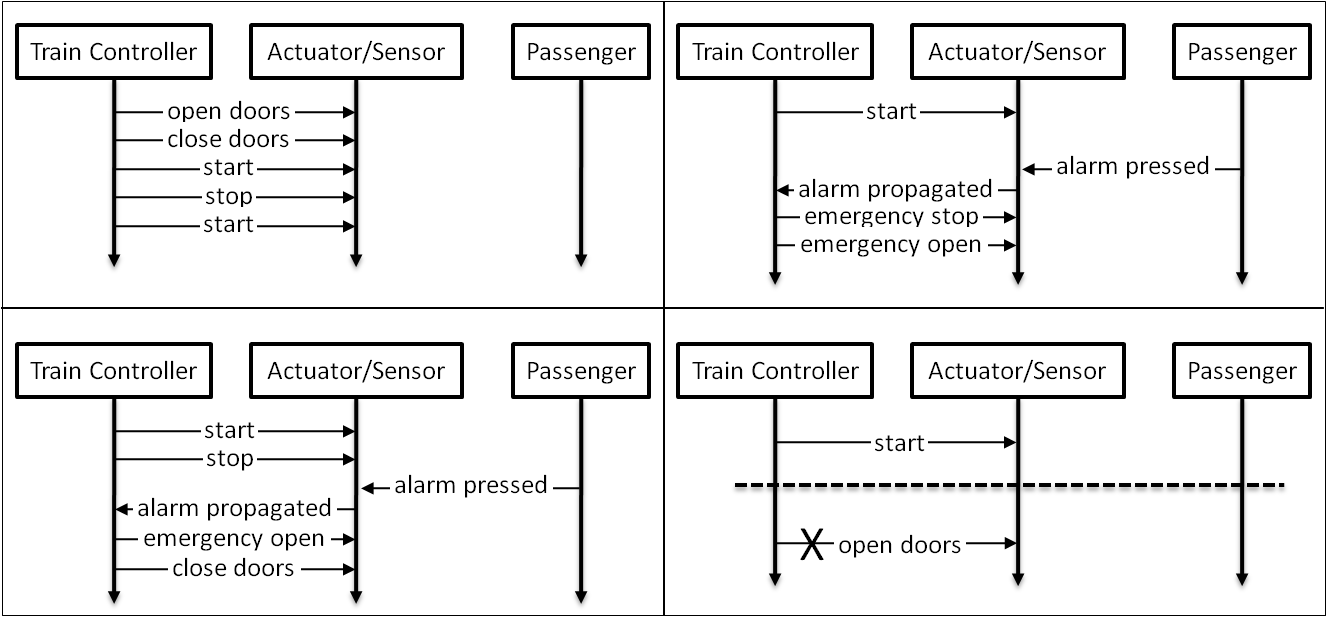
\includegraphics[trim=3mm 3mm 3mm 3mm, clip]{src/4-inductive/images/four-initial-scenarios}}
\caption{Initial positive and negative scenarios for a train system\label{Fig:init:scen}.}
\end{figure}


\item[ChooseStatePair] The candidate solution is refined by merging well- selected state pairs. The \texttt{ChooseStatePair} function determines which pairs to consider. It relies on the standard order $<$ on strings. Each state of the PTA can be labeled by its unique prefix from the initial state. Since prefixes can be sorted according to that order, the states can be ranked accordingly. For example, the PTA states in Fig.~\ref{Fig:algo:steps} are labeled by their rank according to this order. The algorithm considers states $q$ of the PTA in increasing order. The state pairs considered for merging only involve such state $q$ and any state $q'$ of lower rank. The $q'$ states are considered in increasing order as well. This particular ordering is specific to the original RPNI algorithm.

\item[Merge] The \texttt{Merge} function merges the two states $(q, q')$ selected in order to compute a quotient automaton, that is, to generalize the current set of positive behaviors. In the example of Fig.~\ref{Fig:algo:steps}, we assume that states 0, 1, and 2 were previously determined not to be compatible for merging (through negative scenarios initially submitted or generated scenarios that were rejected by the user). Merging a candidate state pair may produce a non-deterministic LTS. For example, after having merged $q = 3$ and $q' = 0$ in the upper part of Fig.~\ref{Fig:algo:steps}, two transitions labeled \texttt{start} from state 0 lead to states 2 and 6, respectively. In such a case, the \texttt{Merge} function merges states 2 and 6 and, recursively, any further pair of states that introduces non-determinism. 

We call \textsl{merging for determinization} this recursive operation of removing non-determinism. This operation guarantees that the current solution at any step is deterministic. It produces an automaton which may accept a more general language than the one it starts from. Therefore, it is not equivalent to the standard algorithm to transform a non deterministic automaton into a deterministic one accepting the same language~\cite{Hopcroft:1979}. Notably, the time complexity of merging for determinization is a linear function of the number of states of the automaton it starts from whereas the standard determinization algorithm is exponential in the worst case. Also, the resulting automaton is still part of the same inductive search space (see Section~\ref{subsection:gi-background-search-space}). 

\begin{figure}
\centering
\scalebox{.67}{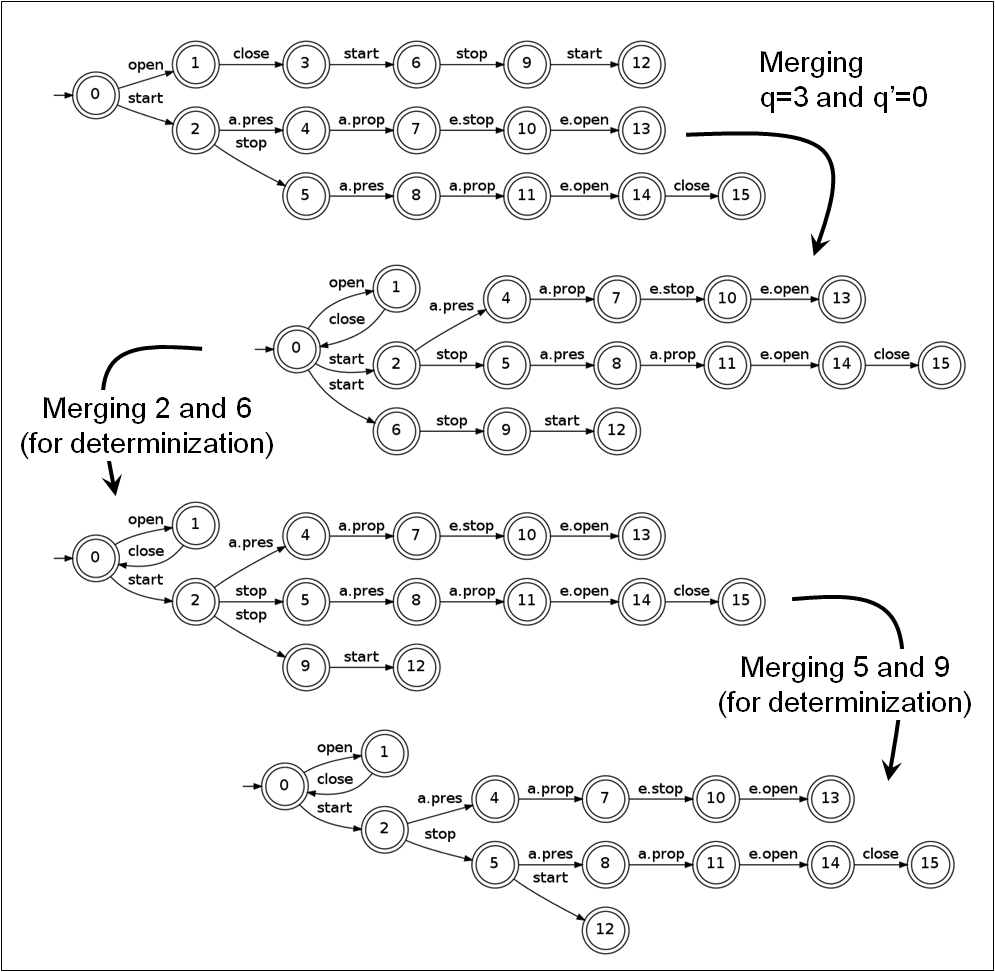
\includegraphics[trim=3mm 3mm 3mm 3mm, clip]{src/4-inductive/images/algo-steps}}
\caption{A typical induction step of the \textsc{QSM} algorithm\label{Fig:algo:steps}.}
\end{figure}

When two states are merged, the rank of the resulting state is defined as the lowest rank of the pair; in particular, the rank of the merged state when merging $q$ and $q'$ is defined as the rank of $q'$ by construction. If no compatible merging can be found between $q$ and any of its predecessor states according to $<$, state $q$ is said to be \textsl{consolidated}. In the example, states 0, 1, and 2 are consolidated.

\item[Consistent] The \texttt{Consistent} function checks whether the automaton $A_{new}$ correctly rejects all negative scenarios. As seen in the pseudo code, the quotient automaton is discarded by \textsc{QSM} when it is detected not to be consistent.

\end{description}

\subsection{Generating queries submitted to the end-user\label{QSM:query}}

This section describes how queries are generated in the \textsc{QSM} algorithm and how the answers provided by the end-user are processed.

\begin{description}

\item[GenerateQuery] When an intermediate solution is consistent with the available scenarios, new scenarios are generated for classification by the end-user as positive or negative. The aim is to avoid poor generalizations by enriching the possibly limited collection of initial scenarios. The notion of characteristic sample drives the identification of which new scenarios should be generated as queries. 

Recall from section~\ref{subsection:gi-background-rpni} that a sample is characteristic of a regular language $L$ if it contains enough positive and negative information. On the one hand, the required positive information is the set of short prefixes $Sp(L)$ which form the shortest histories leading to each state of the canonical automaton $A(L)$. This positive information must also include all elements of the kernel $N(L)$ which represents all system transitions, that is, all shortest histories followed by any admissible event. If such positive information is available, $A(L)$ can always be derived from the PTA by an appropriate set of merging operations. On the other hand, the negative traces provide the necessary information to make incompatible the merging of states which should be kept distinct. A negative trace which would exclude the merging of a state pair $(q, q')$ can be simply made of the shortest history leading to $q'$ followed by any continuation from state $q$ as detailed below.

Consider the current solution of our induction algorithm when a pair of states $(q, q')$ is selected for merging (line 5 in the pseudo code). By construction, $q'$ is always a consolidated state at this step of the algorithm; that is, $q'$ is considered to be in $Sp(L)$. State $q$ is always both the root of a tree and the child of a consolidated state. In other words, $q$ is situated at one letter of a consolidated state, that is, $q$ is considered to be in $N(L)$. States $q$ and $q'$ are compatible according to the available negative scenarios; they would be merged by the standard RPNI algorithm. The QSM extension will first confirm or infirm the compatibility of $q$ and $q'$ by generating scenarios to be classified by the end-user. The generated scenarios are constructed as follows.

\begin{figure}
\centering
\scalebox{.75}{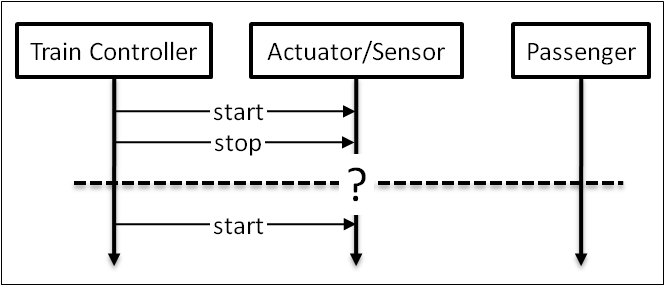
\includegraphics[trim=3mm 3mm 3mm 3mm, clip]{src/4-inductive/images/scenario-question}}
\caption{A new scenario to be classified by the end-user\label{Fig:generated:question}.}
\end{figure}

Let $A$ denote the current solution, $L(A)$ the language generated by $A$, and $A_{new}$ the quotient automaton computed by the \texttt{Merge} function at some given step. Let $x \in Sp(L)$ and $y \in N(L)$ denote the short prefixes of $q'$ and $q$ in A, respectively. Let $u \in L(A)/y$ denote a suffix of $q$ in $A$. 

A generated scenario is built from a system trace $xu$ such that $xu \in L(A_{new})\setminus L(A)$; it can be further decomposed as $xvw$ such that $xv \in L(A)$. The trace $xu$ is thus constructed as the short prefix of $q'$ concatenated with a suffix of $q$ in the current solution, provided the entire behavior is not yet accepted by $A$. Such system trace can be converted to MSC using the structural information provided by a context diagram \cite{Jackson:1995}. The scenario is made of two parts: the first part $xv$ is an already accepted behavior whereas the second part $w$ provides a continuation to be checked for acceptance by the end-user. When submitted to the end-user, the generated scenario can always be rephrased as a question: after having executed the first episode ($xv$), can the system continue with the second episode ($w$)? 

Consider the example in Fig.~\ref{Fig:algo:steps} with selected state pair $q=3, q'=0$. As $q'$ is the root of the PTA, its short prefix is the empty trace $\lambda$. The suffixes of $q$ here yield one generated question (Fig.~\ref{Fig:generated:question}), which can be rephrased as follows: when having started and stopped the train, can the controller restart it? One can see that the first episode of this scenario in Fig.~\ref{Fig:algo:steps} is already accepted by $A$ whereas the entire behavior is accepted in $A_{new}$.

\item[CheckWithEndUser] When a new scenario is generated, it is submitted as a query to the end-user. If the end-user classifies the $Query$ as positive, it is added to the collection of positive scenarios. This addition changes the search space as it extends $S^+$ and consequently the PTA. However, this extension is implicit as the new solution $A_{new}$ is, by construction, also a quotient automaton of this extended PTA. When the $Query$ is classified as negative the induction process is recursively started on the extended scenario collection.

\end{description}

The QSM algorithm has a polynomial time complexity in the size of the learning sample $\mathcal{L}^+(Sc)$, see \cite{Dupont:2008}. 

Moreover, when it receives a characteristic sample in the initial scenario collection it is guaranteed that no additional scenario can be classified as negative. It follows that QSM will not be called recursively anymore and stops by returning the target model. 

An experimental study of the actual sample size required to observe the convergence of \textsc{QSM} and the number of queries submitted to the end-user is detailed in Chapter~\ref{chapter:evaluation}.

\subsection{Reducing the number of queries; the blue-fringe optimization\label{BlueFringe}}

The order in which states are considered for merging by the \texttt{ChooseStatePair} function described in section~\ref{QSM:merging} follows from the implicit assumption that the current sample is characteristic. Consequently, two states are considered compatible for merging if there is no suffix to distinguish among them. This can lead to a significant number of scenarios being generated to the end-user when the initial sample is sparse and actually not characteristic for the target System LTS. 

To overcome this problem, one can use an optimized strategy known as Blue-Fringe~\cite{Lang:1998}. The difference lies in the way state pairs are considered for merging. The general idea is to early detect incompatible state pairs and, subsequently, first consider state pairs for which compatibility has the highest chance to be confirmed by the user through positive classification. The resulting ``please confirm'' interaction may also appear more appealing to the user.

\begin{figure}
\centering
\scalebox{.55}{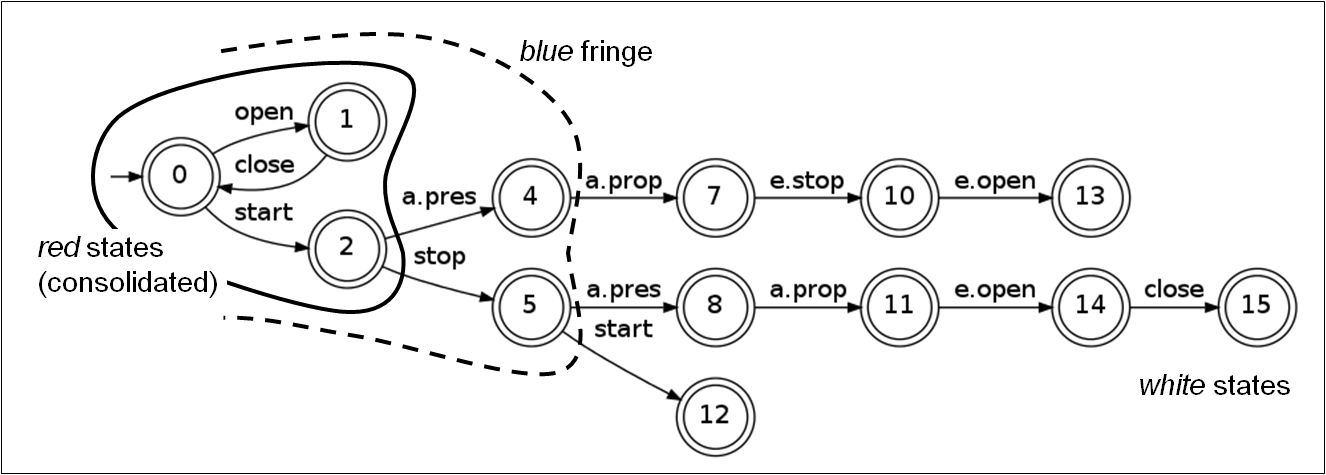
\includegraphics[trim=3mm 3mm 3mm 3mm, clip]{src/4-inductive/images/blue-fringe}}
\caption{Consolidated states (red) and states on the fringe (blue) in a temporary solution\label{Fig:BlueFringe}.}
\end{figure}

Fig.~\ref{Fig:BlueFringe} gives a typical example of a temporary solution produced by the original algorithm. Three state classes can be distinguished in this LTS. The red states are the consolidated ones (0, 1 and 2 in this example). Outgoing transitions from red states lead to blue states unless the latter have already been labeled as red. Blue states form the blue fringe (4 and 5 in this case). All other states are white states. 

The original \texttt{ChooseStatePair} function described in section~\ref{QSM:merging} considers the lowest-rank blue state first (state 4 here) for merge with the lowest-rank red state (0). When this choice leads to a compatible quotient automaton, generated scenarios are submitted to the end-user; in this case, a scenario equivalent to the trace \artifact{<alarm propagated, emergency stop, emergency open>}. The above strategy may lead to multiple queries being generated to avoid poor generalization. Moreover, such queries may be non-intuitive for the user, \textit{e.g.} the \artifact{alarm propagated} event is sent to the train controller without having been fired by the \artifact{alarm pressed} event to the sensor.

To select a state pair for merging, the Blue-Fringe strategy evaluates all (red, blue) state pairs first. The \texttt{ChooseStatePair} function now calls the \texttt{Merge} and \texttt{Compatible} functions before selecting the next state pair. If a blue state is found to be incompatible with all current red states, it is immediately promoted to red; the blue fringe is updated accordingly and the process of evaluating all (red, blue) pairs is iterated. When no blue state is found to be incompatible with red states, the most compatible (red, blue) pair is selected for merging. This is dictated by a scoring mechanism implemented in the \texttt{Compatible} function (see below).

For implementing the Blue-Fringe strategy, it is convenient to adapt \texttt{Initialize} so as to build an \emph{augmented} prefix tree acceptor. Such PTA captures the negative traces in $\mathcal{L}^-(Sc)$ in addition to the positive traces in $\mathcal{L}^+(Sc)$. States reached by a negative trace are tagged as error states; they are depicted in black, as in Fig. \ref{figure:augmented-pta}. 

The \texttt{Compatible} function is also updated to return a compatibility score instead of a boolean value. The score is defined as $-\infty$ when merging the current (red, blue) pair leads to merge an accepting state and an error state during merging for determinization\footnote{in the case of a prefix-closed language, non-error states are all accepting. Recall that this is not necessarily true for any regular language.}; this score indicates an incompatible merging. Otherwise, the compatibility score measures how many accepting states have been merged together. The (red, blue) pair with the highest compatibility score is considered first. The strategy can be further refined with a compatibility threshold $\alpha$ as additional input parameter. Two states are considered to be compatible if their compatibility score is above that threshold. This additional parameter controls the level of generalization since increasing $\alpha$ decreases the number of state pairs that are considered compatible for merging; it thus decreases the number of generated queries.

\begin{figure}\centering
\scalebox{.35}{\includegraphics*{src/4-inductive/images/augmented-pta}}
\caption{Augmented PTA for scenarios in Fig.~\ref{Fig:init:scen}\label{figure:augmented-pta}.}
\end{figure}

Experimental results about the effectiveness of using QSM with and without the Blue-Fringe strategy are detailed in Chapter~\ref{chapter:evaluation}.

\section{Using constraints for multi-view consistency\label{section:inductive-mutliview-consistency}}

The interactive QSM algorithm described in Section~\ref{section:lts-induction-from-mscs} provides a system LTS consistent with all available positive and negative scenarios. The Blue-Fringe strategy can also be applied to reduce the number of additional scenarios submitted to the end-user. The latter strategy relies on two equivalence classes partitioning the states of an augmented PTA. These classes correspond to the accepting states and the error states, respectively. All states belonging to the same class are not necessarily merged in the final solution; however, the \texttt{Compatible} function guarantees that only states belonging to the same class \emph{can} be merged.

This approach can be extended to achieve multi-view consistency by incorporating various sources of information. Such information refines the equivalence partition and further constrains the compatible merging operations. Injecting knowledge-based constraints has many advantages: 
\begin{itemize}
\item It ensures strong consistency of the system LTS with other views;
\item It reduces the number of scenario queries in the interactive setting;
\item It speeds up the search.
\end{itemize}

Section \ref{subsection:induction-pruning-with-domain-knowledge} shows how to incorporate domain knowledge such as fluent definitions. Section \ref{subsection:induction-pruning-with-goals} shows how goals can be used to constrain the generalization. 

The optimization techniques detailed hereafter are based on various equivalence relations over system states. The term \emph{equivalence relation} is used here in its usual mathematical sense, namely, a symmetric, reflexive, and transitive binary relation over states. The general principle underlying our techniques is the following:
\begin{quote}
\emph{Two states will be considered for merging if they agree according to all considered equivalence relations.}
\end{quote}

%%%%%

\subsection{Injecting domain knowledge\label{subsection:induction-pruning-with-domain-knowledge}}

The domain knowledge used to constrain state merging comes from multiple sources: 
\begin{itemize}
\item Fluent definitions;
\item Knowledge about components in the environment of the software-to-be;
\item Specifications of domain properties.
\end{itemize}
We discuss them successively.

%%

\subsubsection*{Propagating fluents}

Fluent definitions provide simple and easy-to-provide domain descriptions to constrain induction. For example, the definition
\begin{center}
fluent $DoorsClosed = \textless \{$close doors$\}, \newline
 \{$open doors, emergency open$\} \textgreater $ initially $true$ \\
\end{center}
describes train door states as being either closed ($DoorsClosed = true$) or open ($DoorsClosed = false$); it also states which event is responsible for which state change. 

Such descriptions can be effectively used to constrain the induction process so that the synthesized System LTS conforms to them. The idea is to decorate each state of the PTA with the value of every fluent. This can be done using a symbolic execution algorithm \cite{Damas:2006, Damas:2011} (see Section~\ref{section:background-fluents}).

The pruning rule for constraining the induction process is here to \emph{avoid merging inconsistent states} according to these decorations. 

The specific equivalence relation is thus the set of state pairs where both states have the same fluent value assignment. The decoration of the merged state is simply inherited from the states being merged.
\begin{quote}
\emph{Two states will be considered for merging if they have the same value for every fluent.}
\end{quote}

Fig.~\ref{dc-augmented-pta} shows the result of propagating the values of the fluent \emph{DoorsClosed} along the augmented PTA built from the scenarios described in Fig.~\ref{Fig:init:scen}.

\begin{figure}
\centering
\scalebox{.33}{\includegraphics*{src/4-inductive/images/dc-augmented-pta}}
\caption{Propagating fluents along the PTA to prune the inductive search space\label{dc-augmented-pta} (DC stands for \emph{DoorsClosed})}
\end{figure}

%%

\subsubsection*{Unfolding models of external components}

Quite often the components being modeled need to interact with other components in their environment - \textit{e.g.}, legacy components in a bigger existing system, foreign components in an open system, etc. In such cases the behavior of external components is generally known - typically, through some behavioral model \cite{Hall:2004}. External components are assumed here to be known by their LTS model. 

For example, Fig.~\ref{Fig.:alarm-sensor} shows the LTS for a legacy alarm sensor in our train system. When the alarm button is pressed by a passenger, this component propagates a corresponding signal to the train controller. 

\begin{figure}
\centering
\scalebox{.4}{\includegraphics*{src/4-inductive/images/alarm-sensor}}
\caption{LTS model for an alarm sensor\label{Fig.:alarm-sensor}.}
\end{figure}

A LTS model of an external component can constrain the induction process so that the synthesized system LTS conforms to it. The idea is to decorate the PTA with states of the external LTS by unfolding the latter onto the PTA. Such decoration is performed by jointly visiting the PTA and the external LTS; the latter synchronizes on shared events and remains in its current state on other events.

Fig.~\ref{Fig.:alarm-unfolded-pta} shows the result of unfolding the alarm sensor LTS from Fig.~\ref{Fig.:alarm-sensor} on the augmented PTA built from the scenarios described in Fig.~\ref{Fig:init:scen}. Each state of the PTA is labeled with the number of the corresponding state in the alarm sensor LTS. 

\begin{figure}
\centering
\scalebox{.35}{\includegraphics*{src/4-inductive/images/alarm-unfolded-pta}}
\caption{Unfolding the alarm sensor LTS onto the PTA\label{Fig.:alarm-unfolded-pta}.}
\end{figure}

The pruning rule for constraining the induction process is now to \emph{avoid merging states decorated with distinct states of the external component}. The specific equivalence relation used here is the set of states where both states have the same external LTS state. 

\begin{quote}
\emph{Two states will be considered for merging if they have the same external LTS state.}
\end{quote}

%%

\subsubsection*{Using declarative domain properties}

Descriptive statements and assumptions about the domain can be expressed declaratively in FLTL (see Section~\ref{section:background-goals}). For example, the physical law
\begin{align*}
\square(HighSpeed \rightarrow Moving)
\end{align*}
\noindent excludes all negative traces where the train is running at high speed while not moving. 

The technique for constraining induction through descriptive or prescriptive statements is the same; we discuss it hereafter.

%%%%%

\subsection{Injecting goals\label{subsection:induction-pruning-with-goals}}

For reasons discussed in Section \ref{section:background-goals}, we restrict our attention to goals and domain properties that can be formalized as pure FLTL safety properties. Remember that these properties refer to  ``\emph{something bad may never happen}''.

Consider the following goal requiring train doors to remain closed while the train is moving:
\begin{center}
\artifact{Maintain[DoorsClosed While Moving]} = $\square(Moving \rightarrow DoorsClosed)$
\end{center}

Fig.~\ref{Fig.:tester-automaton-inductive} shows the tester automaton for this property (cfr. Section \ref{subsection:background-property-and-tester-automata}). The accepting state of this tester captures all traces violating the safety property; any trace leading to it corresponds to an undesired system behavior. In particular, the trace \artifact{<start, open>} corresponds to the initial negative scenario in Fig.~\ref{Fig:init:scen}. As seen in Fig.~\ref{Fig.:tester-automaton-inductive}, the tester provides many more negative traces. Property testers can in fact provide potentially infinite classes of negative scenarios.

\begin{figure}
\centering
\scalebox{.35}{\includegraphics*{src/4-inductive/images/tester-automaton}}
\caption{Tester LTS for the goal \artifact{Maintain[DoorsClosed While Moving]}.\label{Fig.:tester-automaton-inductive}}
\end{figure}

The property tester is used to constrain the induction process in a way similar to an external component LTS. The PTA and the tester are traversed jointly in order to decorate each PTA state with the corresponding tester state. Fig.~\ref{Fig.:goal-unfolded-pta} shows the PTA decorated using the tester of Fig.~\ref{Fig.:tester-automaton-inductive}.

\begin{figure}
\centering
\scalebox{.35}{\includegraphics*{src/4-inductive/images/goal-unfolded-pta}}
\caption{Augmented PTA decorated using the tester automaton from Fig.~\ref{Fig.:tester-automaton-inductive}\label{Fig.:goal-unfolded-pta}.}
\end{figure}

The pruning rule for constraining the induction process is now to \emph{avoid merging states decorated with distinct states of the property tester}. The specific equivalence relation used here is the set of states where both states correspond to the same state of the property tester. 
\begin{quote}
\emph{Two states will be considered for merging if they have the same property tester state.}
\end{quote}

This pruning technique guarantees the consistency between the synthesized System LTS and the considered goals and domain properties. In other words, for every goal or domain property $G$ injected in the synthesis process, the following consistency condition holds (see Section \ref{subsection:background-goals-consistency}):
\begin{align*}
\mathcal{L}^-(G) \cap \mathcal{L}(System) &= \emptyset,
\end{align*}
where \emph{System} here denotes the synthesized system LTS and $\mathcal{L}^-(G)$ captures all traces violating $G$.

Note that the guarantee given by the above condition is weaker than the \emph{consistent system view} condition (\ref{relation:inductive-statement-negative}) in Section \ref{subsection:inductive-synthesis-statement}. The latter requires the consistency of the synthesized system $\system$ while the above condition only applies to the system LTS. As with implied negative scenarios, a goal could be satisfied by the synthesized System LTS while being violated by the real distributed system. This issue is further discussed in Section \ref{section:inductive-discussion}.

\subsection{Discussion\label{subsection:qsm-constraints-implementation-notes}}

The equivalence relations considered in the previous sections are all invariant under state merging. In other words, a state derived by merging some states simply inherits their relation. This allows each relation to be computed only once on the initial PTA; the results of such pre-processing are kept as annotations on PTA states. 

Our implementation reuses the decoration algorithm from \cite{Damas:2006} to propagate fluent values on the PTA (see Section~\ref{subsection:fluents-along-multiple-traces}). Its generalization in~\cite{Damas:2011} may be used as an effective mean to unfold models of legacy components and tester automata on the PTA without additional developments.

The principle for constraining state merging through equivalence relations first appeared in~\cite{Coste:1998, Coste:2004}. It can be further instantiated to other equivalence relations not considered here. In particular, it is \emph{not} limited to relations that are invariant under state merging.

As an illustrative example, consider the following generalization of the way fluent values are used to constrain the induction process. We know from Section~\ref{subsection:fluents-along-multiple-traces} that the states of any LTS can be annotated with invariants defined on fluents. Let $inv$ denote the function mapping each PTA state to its state invariant; let also denote by \emph{Dom} a domain property that must be met in every state of the system LTS. Consider the following pruning rule:
\begin{quote}
\emph{Two states $q$ and $q'$ will be considered for merging if $inv(q) \wedge inv(q') \models \mbox{Dom}$}
\end{quote}

The equivalence relation here is the set of state pairs whose conjunction of invariants satisfies the domain property. This equivalence relation is \emph{not} invariant under state merging. The merging constraint can however be enforced; to achieve this, the compound state resulting from merging $q$ and $q'$ has to be annotated by the conjunction of their state invariants; this new invariant is then used in subsequent state merging.

In the general case of DFA induction\footnote{that is, in contrast to LTS induction}, a similar mechanism is needed to implement the Blue-fringe optimization with an augmented PTA. In that case, an error state may be merged with a non accepting state provided the result is not merged later with an accepting one. That is, the relation capturing the equivalence of states in terms of their continations is not invariant under state merging.

\section{LTS synthesis from high-level MSCs\label{section:inductive-from-hMSC}}

The previous sections have shown how system behaviors specified in collections of MSC scenarios can be first generalized as a System LTS, then decomposed as a set of agent LTSs. The technique supports the incremental enrichment of an initial scenario collection through scenario queries. It also takes other models into account, such as goals, so as to preserve multi-view consistency. Behavior generalization, incremental synthesis and multi-view consistency are the three main requirements identified in Section \ref{subsection:inductive-synthesis-requirements}. 

Coupled with other synthesis techniques such as goal mining from scenarios\footnote{whose simplest form consists in asking ``why'' when facing with a negative scenario.} \cite{Damas:2006}, interactive LTS induction is really effective; starting from a small initial scenario collection, richer system models can be synthesized in only a few iterations. Chapters~\ref{chapter:evaluation} and \ref{chapter:tool-support} illustrate this claim with evaluations and overview of the tool support.

However, for any non-toy system, a large scenario collection might become unmanageable. Among others, consistency of the collection might be difficult to guarantee without costly refactoring on scenarios. One reason is that all scenarios of a collection are required to start in the same system state; this usually implies a lot of redundancy in system descriptions.

One way to tackle this problem is to use high-level message sequence charts (hMSCs) for structuring scenario descriptions. As detailed in Section \ref{subsection:background-hmsc}, hMSCs are directed graphs where each node refers to a MSC or a finer grained hMSC (see Fig.~\ref{image:train-hmsc}). Scenarios can then be structured by introducing alternatives, sequences and loops.

Having a structured form of scenario \emph{helps} specifying a large system with scenarios; it does not \emph{solves} the problem of achieving a complete and consistent view of agent behaviors:
\begin{itemize}
\item capturing all possible interleavings of a distributed system proves difficult with scenarios; a hMSC is therefore hardly complete in practice,
\item complementary features of a system deserve being specified in complementary models; in addition to using multiple system views, having system behaviors specified in more than one hMSC makes sense.
\end{itemize}

Having a synthesis technique to merge and to generalize behaviors described in hMSCs seems a convenient extension to the synthesis technique described so far. For this, the LTS synthesis statement is first revisited in Section~\ref{subsection:hmsc-induction-problem-revisited}. The inductive algorithm is then adapted in Section \ref{subsection:hmsc-induction-algo-adaptation}.

\subsection{Revisiting the LTS synthesis statement\label{subsection:hmsc-induction-problem-revisited}}

Merging multiple hMSCs $H_1,\ldots,H_n$ with respect to trace behaviors simply amounts to compute the union of their respective languages. This is equivalent to building a new hMSC $H$ reaching the finer-grained $H_1,\ldots,H_n$ from its initial state. Additional positive scenarios $S^+_1,\ldots,S^+_n$, typically coming from scenario queries, could be integrated in a similar way. This is illustrated in Fig.~\ref{figure:multiple-hmscs}.

\begin{figure}\centering
\scalebox{.70}{
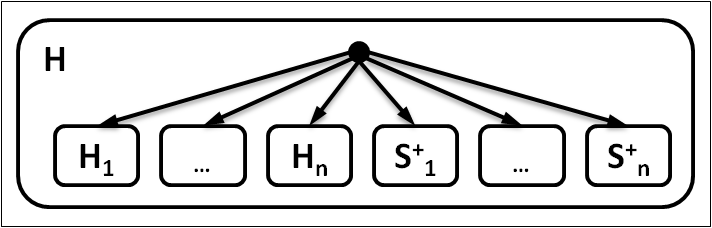
\includegraphics[trim=3mm 3mm 3mm 3mm, clip]{src/4-inductive/images/multiple-hmscs}}
\caption{Merging multiple hMSCs amounts to builds a new one that reaches finer-grained hMSCs from its initial state.\label{figure:multiple-hmscs}} 
\end{figure}

However, a hMSC only permits specifying positive behaviors. As explained in previous sections, negative information is needed to avoid poor generalizations. Negative scenarios, fluents, goals, etc. all provide a source of negative knowledge that can be used to constraint the induction process. The algorithmic adaptations considered later stay compatible with the constraint mechanism based on equivalence relations on system states.

Without loss of generality therefore, we will assume that behaviors are specified through one hMSC only, complemented with a scenario collection. The latter contains negative scenarios and answers to scenario queries. Under these assumptions, the LTS synthesis statement is restated as follows: 

\begin{quote}
\underline{Given}~a hMSC $H$ and a scenario collection $Sc = (S^+,S^-)$ consistent with each other
\begin{align*}
[\mathcal{L}^+(Sc) \cup \mathcal{L}(H)] \cap \mathcal{L}^-(Sc) &= \emptyset
\end{align*}
\underline{Synthesize}~the system as a composition of agent LTSs
\begin{align*}
System = (Ag_1 \parallel \ldots \parallel Ag_n)
\end{align*}
\underline{Such that}~$H$, $Sc$ and $System$ are consistent.
\end{quote}

The hMSC trace semantics is left open in the formulation above. In other words, one has to decide which set of behaviors does $\mathcal{L}(H)$ denote. We recall below the relations between the three hMSC languages covered in Section \ref{subsection:background-hmsc}: 
\begin{align}
\mathcal{L}_{strong}(H) \subseteq \mathcal{L}_{weak}(H) &\subseteq \mathcal{L}_{arch}(H)
\end{align}

$\mathcal{L}_{strong}(H)$ denotes the set of system behaviors with strong sequential composition of hMSC nodes and total event ordering inside MSCs. It is the simplest and most intuitive model for stakeholders involved in early phases of system design. However, it supposes an implicit synchronization scheme used by the agents that is usually not available in real distributed systems. $\mathcal{L}_{arch}(H)$ is the most realistic for such systems, as it captures all possible interleavings of agent behaviors. $\mathcal{L}_{weak}(H)$ is mainly used for explaining and detecting implied scenarios in hMSC specifications \cite{Uchitel:2003}; it is also the hardest to compute.

Making a choice of semantics is required for generalizing behaviors because inductive synthesis takes a set of traces as input. The chosen semantics must of course fit domain assumptions. From an algorithmic point of view however, the three hMSC languages above require the same adaptations of the inductive process, as explained in the next sections.

\subsection{Generalizing high-level MSC languages\label{subsection:hmsc-induction-algo-adaptation}}

Recall that learning a regular language $L$ aims at generalizing a positive sample $S_+$ under the control of a negative sample $S_-$ such that the following relation of language inclusions holds:
\begin{align}
S_+~~\subseteq~~L~~\subseteq~~\Sigma^*\setminus S_-
\end{align}

LTS synthesis from a scenario collection $Sc$ reduces to grammar induction because the sets $\mathcal{L}^+(Sc)$ and $\mathcal{L}^-(Sc)$ are valid positive and negative samples, respectively (see Section \ref{subsection:inductive-lts-synthesis-reduction}). In particular, they denote \emph{finite} sets of traces.

When considering the generalization of hMSC behaviors, the sets of positive and negative traces are $\mathcal{L}^+(Sc) \cup \mathcal{L}(H)$ and $\mathcal{L}^-(Sc)$, respectively. The positive set is no longer a sample because $\mathcal{L}(H)$ might contain an infinite number of traces. Therefore, the current problem statement no longer fits exactly in the identification in the limit framework presented in Section \ref{section:inductive-background}. 

From a theoretical point of view, it means that generalizing hMSC languages is a different problem than generalizing MSC languages; therefore, further study would be needed to re-state the convergence criteria and the notion of characteristic sample in particular. From an algorithmic point of view, however, only a few adaptations of RPNI and QSM are required. They are explained in the next section.

\subsection{The Automaton State Merging algorithm\label{subsection:automaton-state-merging}}

The algorithm to generalize behaviors specified in a hMSC is given in Algorithm~\ref{ASM}, called Automaton State Merging (ASM). It is very similar to QSM, given in Section~\ref{section:lts-induction-from-mscs}, except that the interactive feature is ommited here (we discuss it later). QSM itself being an interactive extension to RPNI, Algorithm~\ref{ASM} is almost RPNI itself which might appear suprising at first glance.

\begin{algorithm}
{
\vspace{0.2cm}
\KwIn{A high-level MSC $H$ and a scenario collection $Sc = (S_+, S_-)$}
\KwOut{A System LTS, consistent with both $H$ and $Sc$}

$A \leftarrow $ {\tt Initialize($H$, $Sc$)}\\
\While{$(q,q') \leftarrow $ {\tt ChooseStatePair($A$)}}{
$A_{new} \leftarrow$ {\tt Merge$(A,q,q')$}\\
\If{{\tt Consistent$(A_{new}, S_-)$}}{
 $A \leftarrow A_{new}$
}
}
\Return{$A$}}
\vspace{0.2cm}
\caption{\textsc{ASM}, a state-merging algorithm from high-level Message Sequence Charts\label{ASM}}
\end{algorithm}

The main difference between RPNI and QSM on one side and ASM on the other side is the initial automaton solution built by \texttt{Initialize}. RPNI and QSM initially convert the input \emph{sample} as a PTA, hence a tree, whereas ASM converts the input \emph{language} of the hMSC as a DFA, hence an graph. The main loop of the ASM algorithm can then be seen as generalizing any regular language, under the control of a negative sample; hence the ``Automaton State Merging'' name. A few adaptations are however required to the different functions of the algorithm: 

\begin{description}

\item[Initialize] This function is adapted to return a DFA instead of a PTA. On one side, the positive traces from the hMSC may be captured through a LTS as discussed in Section \ref{subsection:background-hmsc}, provided a choice of hMSC semantics. On the other side, the scenario collection can be captured through a PTA. These two automata can be merged through standard algorithms for capturing the union of regular languages \cite{Hopcroft:1979}. 

In order to use the Blue-Fringe heuristic (see below), the obtained DFA may be augmented with error states encoding the negative sample given by $S_-$. 

\item[ChooseStatePair] In order to preserve the merging order used by RPNI, this function must be slightly adapted. The idea is to pre-compute the natural order among the states of the initial DFA solution. A breadth first search is used and each of them is numbered when encountered. 

Not that the Blue-Fringe strategy does not require special support. The distinction between red and blue states does not rely on any assumption about the initial solution being a tree; in particular, the fact that a fringe state is the root of a tree in RPNI and QSM is incidental (see \texttt{Merge} below).

\item[Merge] The merging for determinization process is often implemented assuming a tree invariant property. This property states that, when considering two states to be merged, at least one of them is the root of a tree. Such a property holds for RPNI and QSM, even when the Blue-Fringe optimization is used. It is a sufficient condition for the determinization process to be finite. 

Even though it is convenient, the tree invariant property is not required, as explained in \cite{Lambeau:2008}. The main merging loop and the \texttt{Merge} function can be implemented without the tree invariant property because the recursive determinization process stops naturally on the first DFA encountered. This observation allows one to start from an arbitrary DFA and, as soon as non-determinism occurs, to reduce it. 
%Fig.~\ref{figure:merging-for-determ-on-dfa} gives an example of such a recursive operation.

\end{description}

The interactive feature of QSM could be easily adapted and plugged to ASM. It consist in replaincing the main loop ASM by the one of QSM (see Algorithm~\ref{QSM} in Section~\ref{section:lts-induction-from-mscs}). In the latter, the \texttt{GenerateQuery} function must be adapted as follows:

\begin{description}

\item[GenerateQuery] The generation of scenario queries relies on the tree invariant property mentioned above. When merging a state pair $(q,q')$, a scenario query is built with the shortest trace leading to $q$ concatenated with the suffixes of $q'$. When $q'$ is the root of a tree, generating a finite scenario is straightforward.

If the tree invariant property no longer holds, the \texttt{GenerateQuery} function must be extended with a procedure for extracting finite suffixes from $q'$. This does not introduce any technical issues; for example, pre-computing a spanning tree on the initial DFA would associate finite suffixes to each of its state. However, what forms a ``good'' suffix for convergence and scenario classification by end-users is an open question. As the adapted algorithm no longer fits in the identification in the limit framework, the notion of a characteristic sample would need to be adapted. 

\end{description}

%\begin{figure}\centering
%\scalebox{.34}{
%\includegraphics*{src/4-inductive/images/merging-for-determ-on-dfa}}
%\caption{Recursive determinization process. States \{3\} and \{0\} of an arbitrary DFA are merged, which causes a non-determinism on letter $b$ from state \{0,3\}. The destination states \{2\} and \{4\} are subsequently merged to reduce the non-determinism.\label{figure:merging-for-determ-on-dfa}} 
%\end{figure}

From a grammar induction point of view, the ASM algorithm can be seen as generalizing any positive regular language $\mathcal{L}^+$ under the control of a negative sample $S_-$. As such, RPNI is thus a special case where the positive language forms a sample $S_+$, that is a finite set of strings.

Interrestingly, the constraint mechanism from Section~\ref{section:inductive-mutliview-consistency} to prune the induction search space and guarantee multi-view consistency can still be used with ASM. Indeed, the partitionning of PTA states according to equivalence relations extracted from domain knowledge can be performed on the input DFA returned by \texttt{Initialize}, \emph{mutatis mutandis}. 

In particular, goals and domain properties can still be used to prune the induction search space, as explained in Section~\ref{subsection:induction-pruning-with-goals}. As goals actually capture negative languages through their tester automaton, this amounts to consider yet another generalization of ASM to generalize a positive language $\mathcal{L}^+$ under the control of a negative one $\mathcal{L}^-$. This generalization is called ASM$^*$ and briefly discussed in \cite{Lambeau:2008}.



\section{Correctness\label{section:inductive-correctness}}

Proving the correctness of our synthesis approach amounts to show that the synthesized system is consistent with both the scenarios and all domain knowledge taken in input. We discuss proof arguments for the different algorithm settings, starting with the simplest case of RPNI-based synthesis and gradually integrating features such as scenario questions and injection of domain knowledge.

\begin{figure}\centering
\scalebox{.65}{
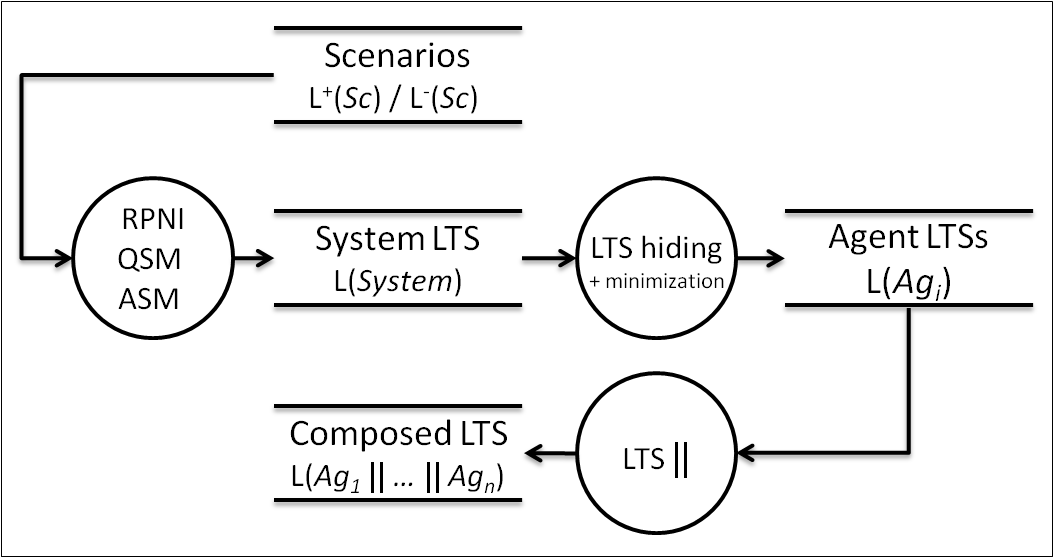
\includegraphics[trim=3mm 3mm 3mm 3mm, clip]{src/4-inductive/images/synthesis-flow-model}}
\caption{Inductive synthesis steps and products.\label{figure:synthesis-flow-model}} 
\end{figure}

Fig.~\ref{figure:synthesis-flow-model} summarizes our approach by showing used algorithms together with their input/output in terms of behavior models and associated languages. 
\begin{itemize}
\item From scenarios, a system LTS is inferred using either RPNI, QSM or ASM. 
\item LTS hiding and minimization is then used to obtain a canonical state machine for each agent. 
\item From the system view point, the result of our synthesis approach is precisely captured by the composition of those state machines.
\end{itemize}

In this figure and in the following discussions,
\begin{itemize}
\item $Sc = (S^+,S^-)$ denotes the input scenario collection; its positive and negative languages are denoted by $\mathcal{L}^+(Sc)$ and $\mathcal{L}^-(Sc)$, respectively.
\item $\mathcal{L}(\me{System})$ denotes the language captured by the inferred system LTS.
\item $\mathcal{L}(Ag)$ denotes the language of an arbitrary agent $Ag$, as captured by its LTS state machine.
\item $\mathcal{L}(\agentscomposed)$ denotes the language captured by the LTS resulting of the composition of individual agent LTSs.
\end{itemize}

We first restrict our attention to the simplest, non-interactive, RPNI approach. Remember from Section~\ref{subsection:inductive-synthesis-statement} that the specification on our approach requires three conditions to hold on synthesized state machines:
\begin{itemize}
\item The \emph{structural consistency} condition requires input scenarios and synthesized agent state machines to agree on the respective agent interfaces.
\item The \emph{consistent agent view} condition requires each synthesized agent state machine to cover the positive behaviors along the corresponding timeline in the input scenarios.
\begin{align}
\mathcal{L}^+(Sc_{\downarrow Ag}) \subseteq \mathcal{L}(Ag)\mbox{~for each agent $Ag$}\label{proof:consistent-agent-view}
\end{align}
where $Sc_{\downarrow Ag}$ denotes the positive behaviors along $Ag$'s timeline in a scenario collection $Sc = (S^+, S^-)$:
\begin{align}
\mathcal{L}^+(Sc_{\downarrow Ag}) = \bigcup_{P \in S^+} \mathcal{L}(P_{\downarrow Ag})~~\cup~~\bigcup_{N \in S^{-}} \mathcal{L}^{+}(N_{\downarrow Ag})\label{proof:lemma-sc-projection}
\end{align}

This is a a slight generalization of the concept of agent traces along a single scenario timeline $M_{\downarrow Ag}$, introduced in Section~\ref{section:background-scenarios}. Observe that it takes both positive and negative scenarios into account.
\item The \emph{consistent system view} requires the system to cover all positive scenarios and reject all negative ones. 
\begin{align}
&\mathcal{L}^+(Sc) \subseteq \mathcal{L}(\agentscomposed)\label{proof:consistent-system-view-1}\\
&\mathcal{L}^-(Sc) \cap      \mathcal{L}(\agentscomposed) = \emptyset\label{proof:consistent-system-view-2}
\end{align}
\end{itemize}

Section~\ref{subsection:system-lts-consistency} briefly discusses the consistency of the inferred system LTS with the scenarios. This result is then used in Section~\ref{subsection:consistent-agent-view} to show that the decomposition step meets the ``structural consistency'' and the ``consistent agent view'' conditions. The ``consistent system view'' condition is further discussed in Section~\ref{subsection:consistent-system-view}. The discussion is pursued in the presence of scenario questions in Section~\ref{subsection:proof-with-scenario-questions} and with the injection of domain knowledge in Section~\ref{subsection:proof-with-domain-knowledge}. Section~\ref{subsection:correctness-of-asm} closes this section with a discussion about the correctness of ASM.

%%%

\subsection{Consistency of the system LTS\label{subsection:system-lts-consistency}}

This section demonstrates that RPNI yields a system LTS consistent with the input scenario collection. The pseudo code given in Algo.~\ref{QSM} is used, ignoring the scenario questions (lines 5 to 10).

\begin{theorem}
\label{theorem:system-lts-consistency-with-sc}
The system LTS synthesized by RPNI covers all positive scenarios and rejects all negative ones.
\begin{align*}
&\mathcal{L}^+(Sc) \subseteq \mathcal{L}(System)\\
&\mathcal{L}^-(Sc) \cap      \mathcal{L}(System) = \emptyset
\end{align*}

\begin{proof}
This theorem is proven by induction using the following invariant:
\begin{align}
&\mathcal{L}^+(Sc) \subseteq \mathcal{L}(A_i)\label{inv:system-lts-consistency-with-sc-1}\\
&\mathcal{L}^-(Sc) \cap      \mathcal{L}(A_i) = \emptyset\label{inv:system-lts-consistency-with-sc-2}
\end{align}

\begin{description}
\item[Base:] $A_0$ denotes the PTA returned by \emph{Initialize}.

The PTA is the largest DFA accepting the positive language; a precondition states that input scenarios are consistent. Therefore the following conditions hold, entailing the invariant:
\begin{align}
&\mathcal{L}^+(Sc) =    \mathcal{L}(A_0)\\
&\mathcal{L}^-(Sc) \cap \mathcal{L}(A_0) = \emptyset
\end{align}

\item[Inductive step:] $A_i$ is the quotient automaton denoting the current solution at step $i$.

From a solution $A_i$, the next solution $A_{i+1}$ is computed by the \emph{Merge} function (see line 3 in Algo.~\ref{QSM}). The latter computes a quotient automaton. Definition~\ref{definition:quotient-automaton} guarantees that such quotient automaton may only generalize the language of $A_i$. As the condition~(\ref{inv:system-lts-consistency-with-sc-1}) holds for $A_i$, the following condition holds as well:
\begin{align*}
&\mathcal{L}^+(Sc) \subseteq \mathcal{L}(A_i) \subseteq \mathcal{L}(A_{i+1})
\end{align*}

On an other hand, quotient automata are only kept as next solution if consistent with the negative scenarios (see lines 4 and 11). Therefore, the following condition holds when such solution is kept (line 11):
\begin{align*}
&\mathcal{L}^-(Sc) \cap \mathcal{L}(A_{i+1}) = \emptyset
\end{align*}

\end{description}
\end{proof}
\end{theorem}

A detailed proof of the convergence of RPNI towards the canonical target automaton when it receives a characteristic sample can be found in~\cite{Oncina:1993} in the more general case of transducer learning.

%%%

\subsection{Structural consistency and consistent agent view\label{subsection:consistent-agent-view}}

Given the consistency of the system LTS with the positive and negative scenarios, the decomposition step guarantees that the \emph{structural consistency} and the \emph{consistent agent view} both hold.

Structural consistency only requires the LTS hiding step to make use of adequate agent alphabets, as induced from the scenarios themselves or given by a (consistent) structural model. We do not discuss it further. 

For each agent $Ag$, the ``consistent agent view'' condition (\ref{proof:consistent-agent-view}) can be derived from (\ref{proof:consistent-system-view-1}) using the following properties and definitions:
\begin{align}
&\mathcal{L}(X) \subseteq \mathcal{L}(Y) \implies \mathcal{L}(X \setminus I) \subseteq \mathcal{L}(Y \setminus I) \label{proof-agent-consistency-1}\\
&\mathcal{L}^+(Sc_{\downarrow Ag}) = \mathcal{L}^+(Sc \setminus \Sigma_{Ag}^c)\label{proof-agent-consistency-2}\\
&\mathcal{L}(Ag) = \mathcal{L}(System \setminus \Sigma_{Ag}^c)\label{proof-agent-consistency-3}
\end{align}
where $\Sigma_{Ag}^c$ denotes the set of all system events excluding those of $Ag$'s interface.
\begin{itemize}
\item (\ref{proof-agent-consistency-1}) states that behavior inclusion is preserved under LTS hiding; this property follows from material in Section~\ref{subsection:lts-hiding}. 
\item (\ref{proof-agent-consistency-2}) rewrites the left term of (\ref{proof:consistent-agent-view}) in terms of hiding of scenario behaviors\footnote{using an abuse of notation as the hiding operator is defined on LTS, not on scenarios collections.}. It can be derived from (\ref{proof:lemma-sc-projection}) and the definition of $M_{\downarrow Ag}$ (see Section~\ref{subsection:background-positive-scenarios}). 
\item (\ref{proof-agent-consistency-3}) follows from the definition (\ref{definition:decomposition-step}) of decomposition step itself (see Section~\ref{subsection:inductive-synthesis-approach}). 
\end{itemize}

From Theorem~\ref{theorem:system-lts-consistency-with-sc} ensuring the consistency of the system LTS with input scenarios, the following condition is established thanks to (\ref{proof-agent-consistency-1})
\begin{align}
&\mathcal{L}^+(Sc \setminus \Sigma_{Ag}^c) \subseteq \mathcal{L}(System \setminus \Sigma_{Ag}^c)\label{proof:consistent-agent-view-milestone}
\end{align}

The ``consistent agent view'' condition (\ref{proof:consistent-agent-view}) is established by substituing the right terms of (\ref{proof-agent-consistency-2}) and (\ref{proof-agent-consistency-3}) in (\ref{proof:consistent-agent-view-milestone}).

%%%

\subsection{Consistent system view: the problem of implied scenarios\label{subsection:consistent-system-view}}

This section discusses the correctness of the ``consistent system view'' condition. The conditions related to the positive and negative scenarios are discussed in turn.

\begin{theorem}
The synthesized system covers all positive scenarios.
\begin{align*}
&\mathcal{L}^+(Sc) \subseteq \mathcal{L}(\agentscomposed)
\end{align*}

\begin{proof}
This condition results from two main properties of our approach:
\begin{itemize}
\item The synthesized system LTS covers all positive scenario behaviors, as guaranteed by Theorem~\ref{theorem:system-lts-consistency-with-sc}.
\begin{align*}
&\mathcal{L}^+(Sc) \subseteq \mathcal{L}(System)
\end{align*}
\item Projecting the system LTS on agent alphabets and recomposing their LTS afterwards does not restrict behaviors:
\begin{align*}
&\mathcal{L}(\mbox{System}) \subseteq \mathcal{L}(\agentscomposed)
\end{align*}
This latter condition can be derived from the definition of agent languages (\ref{proof-agent-consistency-3}) and properties of LTS hiding and composition operators (see Section~\ref{section:background-state-machines}).
\end{itemize} 

\end{proof}
\end{theorem}

\begin{theorem}
The synthesized system excludes all negatives scenarios.
\begin{align*}
&\mathcal{L}^-(Sc) \cap \mathcal{L}(\agentscomposed) = \emptyset
\end{align*}
\end{theorem}

This theorem would require the composed system to exclude all negative scenarios. Due to the potential presence of implied scenarios, our approach only guarantees the weaker condition given by Theorem~\ref{theorem:system-lts-consistency-with-sc}, namely,
\begin{align*}
&\mathcal{L}^-(Sc) \cap \mathcal{L}(\mbox{System}) = \emptyset
\end{align*}

In other words, the induction algorithm ensures that the system LTS excludes all negative scenarios. This property can however be lost after the decomposition and recomposition steps.

The reason has to be found in the possible occurence of so-called \emph{implied scenarios}. Remember from Section~\ref{subsection:background-hmsc} that implied scenarios may appear when a system is specified globally while implemented component-wise ~\cite{Alur:2000, Uchitel:2004}. In our case, the set of implied scenarios is precisely defined as:
\begin{align*}
\mathcal{L}(\agentscomposed) \setminus \mathcal{L}(\mbox{System})
\end{align*}

When this language is not empty, implied scenarios denote system behaviors that the system LTS does not accept but which are exhibited by the composition of agent LTSs. Implied scenarios appear when, once distributed, the agents lack monitoring abilities to restrict their behavior so as to precisely match the system LTS.

Not all implied scenarios are problematic in practice. In particular, it might happen that all implied scenarios denote desired system behaviors. In that case, the presence of implied scenarios is not problematic and may be seen as the result of a second generalization step due to the decomposition and recomposition of agent LTS. This second generalization step proves useful as it weakens the necessity of having a pure structurally complete scenario collection in the first place.

Negative implied scenarios, that is, counterexamples of desired behaviors, are more problematic. In particular, a behavior trace $t$ could be such that the following conditions hold:
\begin{align}
&t \in \mathcal{L}^-(Sc)\label{implied-1}\\
&t \notin \mathcal{L}(\mbox{System})\label{implied-2}\\
&t \in \mathcal{L}(\agentscomposed)\label{implied-3}
\end{align}
that is, (\ref{implied-1}) $t$ denotes a system behavior explicitly rejected through a negative scenario; it might be a question answered negatively; (\ref{implied-2}) $t$ is correctly rejected by the system LTS; (\ref{implied-3}) $t$ is still be exhibited by the composed system.

In such case, observe the ``consistent system view'' condition is not met as (\ref{proof:consistent-system-view-2}) does not hold. As with other scenario approaches, e.g. \cite{Alur:2000, Uchitel:2004}, our synthesis technique fails to guarantee a consistent system view between scenarios and state machines in presence of negative implied scenarios.

In order to detect such situations, the technique from \cite{Uchitel:2004} could be adapted to enumerate implied scenarios and submit them as additional scenario questions to the user (see Section~\ref{section:related-for-analysis-3}). 

Note that, fixing implied scenario problems requires rethinking the system decomposition into agents and/or refactoring their interfaces. In other words, the root cause of implied scenarios problems has to be found in the structural decomposition of the system, not in the particular technique used to infer state machines from scenarios. 

%%%

\subsection{Correctness in the presence of scenario questions\label{subsection:proof-with-scenario-questions}}

The specification of QSM has been strengthened in Section~\ref{section:lts-induction-from-mscs}. This strengthening required the synthesized system to be consistent with all scenario questions in addition to the initial scenario collection. 

Provided a consistent system LTS is inferred with QSM, the correctness arguments for the \emph{structural consistency} and \emph{consistent agent view} conditions remain unchanged. The discussion about implied scenarios also takes place here. Therefore, we only prove the consistency of the system LTS induced by QSM when scenario questions are taken into account.

\begin{theorem}
The system LTS inferred by QSM is consistent with the scenario collection extended with the answers to all scenario questions.

\begin{proof}
This theorem is proven by induction (cfr. Algo.~\ref{QSM}):
\begin{description}
\item[Base:] The base case captures a QSM run where all scenario questions are answered positively. 

In such case, QSM roughly reduces to RPNI, for which Theorem~\ref{theorem:system-lts-consistency-with-sc} is known to hold. We still need to prove that all scenario questions are thus accepted by the synthesized system LTS. 

Observe that scenarios accepted at line 7 are consistent with the current solution $A_{new}$ (line 4). The system LTS returned by QSM is a quotient automaton of $A_{new}$; Definition \ref{definition:quotient-automaton} therefore ensures that the system LTS accepts those scenarios as well.

\item[Inductive step:] The inductive step captures a run where a rejected scenario yields a tail recursive call (line 10).

The discussion about positively accepted scenarios remains unchanged. The scenario collection is correctly extended (see line 7).

Every time a scenario question is rejected by the oracle, the scenario collection is correctly extended as well (see line 9). Provided the oracle does not make classification errors, as required in preconditions, the scenario collection remains consistent for the tail recursive call taking place at line 10.
\end{description}
\end{proof}
\end{theorem}

%%%

\subsection{Consistency with goals and domain properties\label{subsection:proof-with-domain-knowledge}}

QSM pre- and postconditions have been implicitly strenghtened in Section~\ref{subsection:induction-pruning-with-goals} in order to ensure that the synthesized system does not violate known safety properties. In other words, provided the input scenarios and safety properties are consistent, the following postcondition is required to hold:
\begin{align}
&\mathcal{L}^-(G) \cap \mathcal{L}(\agentscomposed) = \emptyset \mbox{~~for every safety property~G}\label{consistency-of-system-lts-with-goals}
\end{align}

A weaker condition is proven in Theorem~\ref{theorem:system-lts-consistency-with-goals} as implied scenarios may lead to goals being violated after the decomposition and recomposition steps. Lemma~\ref{lemma:qsm-and-tester-prefixes} first provides a useful milestone.

\begin{lemma}
When two states $q$ and $q'$ are considered for merging by QSM, all their prefixes are traces leading to the same state in the tester automaton capturing $\mathcal{L}^-(G)$.\label{lemma:qsm-and-tester-prefixes}
\begin{proof}
We assume the correctness of the joint traversal for annotating the PTA states with their corresponding states in the tester automaton (see Section~\ref{subsection:induction-pruning-with-goals}). QSM only considers the merging of state pairs corresponding to the same state in the tester automaton. The prefixes property thus holds for the first merge considered on the PTA; it is trivially preserved under state merging and therefore holds for every state pair considered from the successive quotient automata.
\end{proof}
\end{lemma}

\begin{theorem}
\label{theorem:system-lts-consistency-with-goals}
The system LTS synthesized by QSM is consistent with available safety properties, that is,
\begin{align*}
&\mathcal{L}^-(G) \cap \mathcal{L}(\emph{System}) = \emptyset \mbox{~~for every safety property~G}
\end{align*}

\begin{proof}
Let $G$ denote a safety property. The proof proceeds by induction on the following loop invariant:
\begin{align*}
\mathcal{L}^-(G) \cap \mathcal{L}(A_i) = \emptyset
\end{align*}

\begin{description}
\item[Base:] $A_0$ denotes the PTA.

The invariant holds for $A_0$ as (a) the preconditions require the scenarios and the goals to be consistent and (b) the PTA does not generalize the positive scenario language.
\begin{align*}
&\mathcal{L}^-(G) \cap \mathcal{L}^+(Sc) = \emptyset\\
&\mathcal{L}(A_0) = \mathcal{L}^+(Sc)
\end{align*}

\item[Inductive step:] Let $A_i$ denote a current solution considered by QSM and suppose that the invariant holds. We show that the invariant holds for $A_{i+1}$, that is, the quotient automaton of $A_i$ obtained by merging a candidate state pair $(q,q')$.

By construction of our constraint mechanism based on equivalent state classes, $q$ and $q'$ correspond to the same state $t$ in the tester automaton capturing $\mathcal{L}^-(G)$ (see Section~\ref{subsection:induction-pruning-with-goals}).

The tester is known to be a canonical automaton, that is, it is minimal and deterministic (see Section~\ref{subsection:background-property-and-tester-automata}). A bijection thus exists between states and accepted trace suffixes\footnote{formally called residual languages} \cite{Hopcroft:1979}. 

Therefore, all accepted traces from $q$ (resp. $q'$) in the current solution $A_i$ are rejected traces from $t$ in the tester automaton. By Lemma~\ref{lemma:qsm-and-tester-prefixes} all prefixes of $q$ in $A_i$ (resp. $q'$) are prefixes of $t$ in the tester. As the invariant holds for $A_i$, their respective suffixes must be disjoint.

When $q$ and $q'$ are merged by QSM, the same lemma guarantees that the suffixes ``gained'' by $q'$ (resp. $q$) do not yield new traces in $A_{i+1}$ that would violate the safety property $G$. In other words, the invariant holds for $A_{i+1}$.
\end{description}
\end{proof}
\end{theorem}

%%%

\subsection{Correctness in the presence of control information\label{subsection:correctness-of-asm}}

The correctness proof for ASM follows the same reasoning as the one presented for RPNI in Theorem~\ref{theorem:system-lts-consistency-with-sc}. Discussions about structural consistent, consistent agent view and implied scenarios remain unchanged. 

\begin{theorem}
The system LTS synthesized by ASM is consistent with the hMSC and the scenario collection taken as input.
\begin{align*}
&[\mathcal{L}(H)   \cup \mathcal{L}^+(Sc)] \subseteq \mathcal{L}(System)\\
&\mathcal{L}^-(Sc) \cap \mathcal{L}(System) = \emptyset
\end{align*}
\begin{proof}
The theorem is proven by induction, using the following invariant:
\begin{align*}
&[\mathcal{L}(H) \cup \mathcal{L}^+(Sc)] \subseteq \mathcal{L}(A_i)\\
&\mathcal{L}^-(Sc) \cap \mathcal{L}(A_i) = \emptyset
\end{align*}

\begin{description}
\item[Base:] $A_0$ denotes the automaton returned by \emph{Initialize}

The \emph{Initialize} function implements the synthesis algorithm detailed in \cite{Uchitel:2003} which does not generalize hMSC behaviors. Moreover, the input hMSC and the positive scenarios are required to be consistent with the negative scenarios. Therefore the following invariant holds:
\begin{align*}
&[\mathcal{L}(H) \cup \mathcal{L}^+(Sc)] = \mathcal{L}(A_0)\\
&\mathcal{L}^-(Sc) \cap \mathcal{L}(A_0) = \emptyset
\end{align*}

\item[Inductive step:]
The main induction loop is similar to the one of RPNI. It considers successive quotient automata, which generalize the language captured by the current solution $A_i$.
\begin{align*}
&[\mathcal{L}(H) \cup \mathcal{L}^+(Sc)] \subseteq \mathcal{L}(A_i) \subseteq \mathcal{L}(A_{i+1})
\end{align*}

As shown in Algo~\ref{ASM}, quotient automata are not kept unless being consistent with the negative scenarios (lines 3 and 4). Therefore, the following condition holds in any case:
\begin{align*}
&\mathcal{L}^-(Sc) \cap \mathcal{L}(A_{i+1}) = \emptyset
\end{align*}

\end{description}
\end{proof}
\end{theorem}


\section{Discussion\label{section:background-discussion}}

\subsection{Model synthesis revisited}




\section*{Summary}

This chapter discussed how grammar induction may be used to synthesize LTS state machines from end-user scenarios. The RPNI algorithm provides a basis to inductively generalize scenario behaviors as a system LTS; the latter is then projected on the alphabet of each agent to obtain their state machines.

QSM extends RPNI with an interactive feature where an end-user classifies generated scenarios as positive or negative examples of desired system behavior. This constrains the induction process towards good behavior generalizations. It also allows completing the initial scenario collection with interesting agent interactions that were not initially explored.

QSM and ASM may be constrained through equivalence relations defined on system states. This mechanism was instantiated to prune the induction process with the definition of fluent state variables, models of legacy components, domain properties, and goals. In addition to guaranteeing the consistency of synthesized state machines with other available models, the injection of such knowledge offers better induction performance and reduces the number of user interactions.

Structured forms of scenario descriptions, such as hMSCs, prove useful for large systems. They overcome a limitation of using scenario collections, namely, the requirement that all scenarios start in the same system state. The induction of agent state machines from structured forms of scenarios led to the ASM algorithm, another extension of RPNI. While our current ASM implementation is rather limited, the chapter showed that the design of an induction algorithm mixing hMSC input, scenario questions, and injection of domain knowledge and goals raises minor issues only.

The transition from RPNI/QSM to ASM raises interesting perspectives for future research. From a grammar induction standpoint, a further extension called ASM$^*$ amounts to consider the generalization of a positive language under the control of a negative one. ASM and ASM$^*$ do not exactly fit in the identification-in-the-limit framework; in particular, the convergence criterion would need to be revisited. From the software engineering standpoint, such work would set a sounder basis for tackling the synthesis of behavior models from structured forms of scenarios and safety properties.

\chapter{Inductive Synthesis of State Machines from Scenarios\label{chapter:inductive-synthesis}}

This chapter presents an inductive approach for synthesizing state machines from scenarios. Section~\ref{section:inductive-objectives-and-approach} characterizes the problem, discusses a few requirements and provides an overview of our solution. Section~\ref{section:inductive-background} provides some required background on grammar induction, the inductive framework on which our techniques are rooted \cite{Gold:1978}. Section~\ref{section:lts-induction-from-mscs} describes an interactive technique for learning LTS models from collections of MSCs. This technique is interactive; the end-user is expected to classify additional scenarios generated by the technique as positive and negative examples of system behavior. In Section~\ref{section:inductive-mutliview-consistency}, fluent, goals and domain properties are injected in the process to enforce inter-model consistency and prune the inductive search space for better performance. Section \ref{section:inductive-from-hMSC} discusses how hMSCs can be used as richer input of the synthesis process. Section \ref{section:inductive-correctness} discusses the correctness of our approach.

\section{Objectives and approach\label{section:evaluation-objectives-and-approach}}

The aim of this chapter is to evaluate our inductive synthesis technique in the light of the thesis objectives. The idea is to check whether our synthesis approach provides an effective way of exploring requirements and conducting system design. Or, in terms of the requirements discussed in Chapter~\ref{chap:introduction},

\begin{quotation}
\emph{How well does it help building \emph{adequate}, \emph{complete}, \emph{consistent} and \emph{precise} models for the target system considered?}
\end{quotation}

Such a question is difficult to answer in absolute terms. Answers can however be provided in two ways:
\begin{enumerate}
\item[a)] By comparing the technique with existing ones, either theoretically or on common benchmarks.
\item[b)] By using the technique in controlled experiments. Here, controlled parameters provide variation points to conduct comparisons.
\end{enumerate}
This chapter focusses on the second way of conducting evaluation. A discussion of how our inductive synthesis approach compares and integrates with existing techniques can be found in Chapter~\ref{chapter:related-work}, thereby completing the evaluation given here.

When our inductive synthesis technique is considered in isolation, the question of how well it performs can already be partially answered. For instance, our technique builds \emph{consistent} models by construction; by design, it also helps \emph{completing} them through scenario questions. However, other related questions cannot be answered so simply:
\begin{itemize}
\item How adequate are the synthesized state machines? 
\item What is the impact of fluent, goal and domain knowledge injection on model adequacy?
\item Is the approach usable by end-users? 
\item How many iterations are needed to obtain models considered complete?
\item Does the inductive technique scales and stays usable on large systems?
\end{itemize}

Controlled experiments have thus been conducted to provide answers to those questions. In practice, two kinds of evaluation have been considered, as reflected by the following sections. The specific evaluation protocols used will be described in each case.
\begin{itemize}

\item Section \ref{section:evaluation-experiments-on-case-studies} discusses evaluations conducted on three case studies involving multiple models. The aim here is to evaluate the feasibility of inductive LTS synthesis in practice. Our ISIS tool presented in Section \ref{section:tool-support-isis} has been used as an effective support for designing and conducting the evaluations described there.

\item Section \ref{section:evaluation-experiments-on-synthetic-data} complements this case-driven evaluation with experiments conducted on random automata and samples. The aim here is to study the performance of QSM and ASM in a more systematic way using synthetic datasets whose size grows significantly beyond the average one of the case studies. This will also allow us to compare our techniques with state-of-the-art induction algorithms. To achieve sound comparisons, our evaluation protocol inspires from a benchmark known as Abbadingo \cite{Lang:1998} (see Section~\ref{subsection:evaluation-synthetic-protocol}).
\end{itemize}

Using the ISIS tool on case-studies provides a first evaluation \emph{in situ}. The overall effectiveness of our multi-view synthesis approach will be illustrated on a typical run. In addition, controlled parameters of the experiments provide comparison points to answer finer-grained evaluation questions. Those controlled parameters are:
\begin{itemize}
\item The size the target system LTS, either because a selected case-study or controlled by a random generation procedure.
\item The heuristics used for state merging: the RPNI search order or the Blue-fringe optimization.
\item The presence of absence of an oracle answering scenario questions.
\item The number of fluents and goals injected to prune the induction process.
\item The use of control information in scenarios and the richness of such knowledge.
\end{itemize}

Three measures have been collected when conducting the various experiments. Those measures have a clear impact on the adequacy and usability of the synthesis technique. Therefore, they allow making the link between the controlled parameters and answers to our evaluation questions.
\begin{description}
\item[Model adequacy] Roughly speaking, \emph{model adequacy} captures \emph{how well} an inferred model matches the expected target behavior model. 

Model adequacy is easy to measure in controlled experiments in which, by design, the target model is then known. Depending on the experiment, we will use either a binary value or a finer-grained one.
\begin{itemize}
\item In the former case, the adequacy measure simply captures whether the learned model is \emph{the same} as the target model or not, in terms of behavioral equivalence (see Definition~\ref{definition:trace-equivalence}).
\item In the latter case, an \emph{accuracy} measure will be used; such measure will range from 0.0 to 1.0 dependent on whether the learned model is considered far or close to the target model. This will be estimated through test samples (see Section~\ref{subsection:evaluation-synthetic-protocol}).
\end{itemize}
Note that adequacy is harder to assess on real-world case studies where the target model is unknown. In practice, human inspection of the learned models is required.

\item[Number of scenario questions] The number of queries generated to the oracle is a key measure for the usability of QSM in practice. 

This is certainly true when the oracle is a human being. A large number of queries might also be a problem with automated oracles; online oracles may be slow, others might be expensive, etc.

\item[Induction time] The time taken to infer a model deserves special attention. While a reasonable induction time is desirable in any case, fast, real-time interactions are required for usability of QSM by a human oracle.
\end{description}

Our experiments were designed to isolate the effect on the three measures above of the orthogonal features of our inductive technique. They quantify the gains and costs of the following ones in particular:
\begin{itemize}
\item The use of an oracle who can answer scenario questions: a gain is expected in model adequacy at the cost of a longer induction time.
\item The use of the Blue-fringe heuristic instead of the RPNI search order: a gain in adequacy is expected as well as a reduction of the number of scenario questions;
\item The use of domain knowledge such as fluent and goals: a gain in adequacy and a reduction of scenario questions should be observed as well;
\item The use of control information encoded into a hMSC: here also, a gain in adequacy is expected.
\end{itemize}


\section{Grammar induction for LTS synthesis\label{section:inductive-background}}

\emph{Inductive learning} aims at finding a theory that generalizes a set of observed examples. In \emph{grammar induction}, the theory to be learned is a formal language and the set of positive examples is made of strings defined on a specific alphabet. A negative sample corresponds to a set of strings not belonging to the target language. When the target language is regular and the learned language is represented by a deterministic finite state automaton (DFA), the problem is known as DFA induction. For a regular language $L$, $A(L)$ will denote its canonical automaton, that is the DFA having the smallest number of states and accepting $L$. For recall, $A(L)$ is unique up to a renumbering of its states \cite{Hopcroft:1979}.

\subsection{DFA identification in the Limit\label{subsection:dfa-identification-in-the-limit}}

\emph{Identification in the limit} is a learning framework in which an increasing sequence of strings is presented to the learning algorithm \cite{Gold:1967}. The strings are randomly drawn and correctly labeled as positive or negative. Learning is successful if the algorithm infers the target language in finite time after having seen finite samples. This framework justifies why successful DFA learning needs both positive and negative strings. Gold showed that the class of regular languages cannot be identified in the limit from positive strings only \cite{Gold:1967}. In practice, convergence in finite time toward an exact solution is often bargained with reasonably fast convergence toward a good approximate solution \cite{Lang:1992}.

\subsection{The search space of DFA induction\label{subsection:gi-background-search-space}}

Generalizing a positive sample $S_+$ can be performed by merging states from an initial automaton that only accepts it.  This initial automaton is called a prefix tree acceptor; it is denoted by denoted by $PTA(S_+)$. It is the largest trimmed DFA accepting exactly $S_+$ (see Fig.~\ref{fig:pta:quotient}). The generalization operation is formally defined through the concept of \emph{quotient automaton}.

\begin{definition}[Quotient automaton]
Given an automaton $A$ and a partition $\pi$ defined on its state set, the quotient automaton $A/\pi$ is obtained by merging all states $q$ belonging to the same partition subset $B(q,\pi)$. A state $B(q,\pi)$ in $A/\pi$ thus corresponds to a subset of the states in $A$. 

A state $B(q,\pi)$ is accepting in $A/\pi$ if and only if at least one state of $B(q,\pi)$ is accepting in $A$. Similarly, there is a transition on the letter $\mathrm{a}$ from state $B(q,\pi)$ to state $B(q',\pi)$ in $A/\pi$ if and only if there is a transition on $\mathrm{a}$ from at least one state of $B(q,\pi)$ to at least one state of $B(q',\pi)$ in $A$. 
\end{definition}

\begin{figure}
\begin{center}
\scalebox{.5}{\includegraphics*{src/4-inductive/images/pta}}
\scalebox{.5}{\includegraphics*{src/4-inductive/images/autoPairB}}
\caption{$PTA(S_+)$ (above) where $S_+ = \{\lambda,a,bb,bba,baab,baaaba\}$ is a structurally complete sample 
for the canonical automaton $A(L)$ (below). $A(L) = PTA(S_+)/\pi$ with $\pi=\{\{0,1,4,6,8,10\},\{2,3,5,7,9\}\}$.\label{fig:pta:quotient}}
\end{center}
\end{figure}

By construction of a quotient automaton, any accepting path in $A$ is also an accepting path in $A/\pi$. It follows that, for any partition $\pi$ of the state set of $A$, $L(A/\pi) \supseteq L(A)$. In words, \textsl{merging states in an automaton generalizes the language it accepts.}
 
Learning a regular language is possible if $S_+$ is representative enough of the unknown language $L$ and if the correct space of possible solutions is searched through. These notions are stated precisely hereafter.

\begin{definition}[Structural completeness] A positive sample $S_+$ of a language $L$ is structurally complete with respect to an automaton $A$ accepting $L$ if, when generating $S_+$ from $A$, every transition of $A$ is used at least once and every final state is used as accepting state of at least one string.
\label{structural:completeness}
\end{definition}

Rather than a requirement on the sample, structural completeness should be considered as a limit on the possible generalizations that are allowed from a sample. If a proposed solution is an automaton in which some transition is never used while parsing the positive sample, no evidence supports the existence of this transition and this solution should be discarded. 

\begin{theorem}[DFA search space]
\label{search:theo}
If a positive sample $S_+$ is structurally complete with respect to a canonical automaton $A(L)$ then there exists a partition of the state set of $PTA(S_+)$ such that $PTA(S_+)/\pi = A(L)$~\cite{Dupont:1994}.
\end{theorem} 

This result defines the search space of the DFA induction problem as the set of all automata which can be obtained by merging states of the PTA. Some automata of this space are not deterministic but an efficient determinization process can enforce the solution to be a DFA (see section~\ref{section:lts-induction-from-mscs}).

Figure~\ref{fig:pta:quotient} presents the prefix tree acceptor (above) built from the sample 
$S_+ = \{\lambda,a,bb,bba,baab,baaaba\}$ which is structurally complete with respect to the canonical automaton (below).
This automaton is a quotient of the PTA for the partition $\pi=\{\{0,1,4,6,8,10\},\{2,3,5,7,9\}\}$ of its state set.

To summarize, learning a regular language $L$ can be performed by identifying the canonical automaton $A(L)$ of $L$ from a positive sample $S_+$. If the sample is structurally complete with respect to this target automaton, it can be derived by merging states of the PTA built from $S_+$. A negative sample $S_-$ is used to guide this search and avoid over-generalization. In the sequel, $||S||$ denotes the sum of the lengths of the strings in a sample $S$.

The size\footnote{Let $n$ be the number of states of $PTA(S_+)$. By construction, $n \in \mathcal{O}(||S_+||)$. The search space size is the number of ways a set of $n$ elements can be partitioned into nonempty subsets. This is called a Bell number $B(n)$. It can be defined by the Dobinski's formula: $B(n) = \frac{1}{e} \sum_{k=0}^{\infty} \frac{k^n}{n!}$. This function grows much faster than $2^n$.} of this search space makes any trivial enumeration algorithm irrelevant for any practical purposes. Moreover, finding a minimal consistent DFA, is a NP-complete problem~\cite{Gold:1978,Angluin:1978}. Interestingly, only a fraction of this space is efficiently searched through by the RPNI algorithm or the \textsc{QSM} algorithm described in Section~\ref{section:lts-induction-from-mscs}.

\subsection{Characteristic samples for the RPNI algorithm\label{subsection:gi-background-rpni}}

We do not fully detail the RPNI algorithm in the present section but the original version forms a particular case
of our interactive algorithm \textsc{QSM}, as discussed in Section~\ref{section:lts-induction-from-mscs}. The convergence of RPNI to the correct automaton $A(L)$ is guaranteed when the algorithm receives a sample as input that includes a \textsl{characteristic sample} of the target language~\cite{Oncina:1992}. A proof of convergence is presented in~\cite{Oncina:1993} in the more general case of transducer learning. Some further notions are needed here.

\begin{definition}[Short prefixes and suffixes] 
Let $Pr(L)$ denote the set of prefixes of $L$, with $Pr(L) = \{u | \exists v, uv \in L\}$. The right-quotient of $L$ by $u$, or set of suffixes of $u$ in $L$, is defined by $L/u = \{v | uv \in L\}$. The set of short prefixes $Sp(L)$ of $L$ is defined by $Sp(L) = \{x \in Pr(L) | \neg\exists u \in \Sigma^*$ with $L/u = L/x$ and $u < x\}$.
\end{definition}

In a canonical automaton $A(L)$ of a language $L$, the set of short prefixes is the set of the first strings in standard order\footnote{The standard order of strings on the alphabet $\Sigma=\{a,b\}$ is $\lambda < a < b < aa < ab < ba < bb < aaa < \ldots$} $<$, each of which leads to a particular state of the canonical automaton. Consequently, there are as many short prefixes as states in $A(L)$. In other words, the short prefixes uniquely identify the states of $A(L)$. The set of short prefixes of the canonical automaton of Fig.~\ref{fig:pta:quotient} is $Sp(L) = \{\lambda, b\}$.

\begin{definition}[Language kernel]
 The kernel $N(L)$ of the language $L$ is defined as $N(L) = \{xa | x \in Sp(L), a \in \Sigma, xa \in Pr(L)\} \cup \{\lambda\}$.
\end{definition}

The kernel is made of the short prefixes extended by one letter, and the empty string. By construction $Sp(L) \subseteq N(L)$. The kernel elements represent the transitions of the canonical automaton $A(L)$ since they are obtained by adding one letter to the short prefixes that represent the states of $A(L)$. The kernel of the language defined by the canonical automaton of Fig.~\ref{fig:pta:quotient} is $N(L) = \{\lambda, a, b, ba, bb\}$.

\begin{definition}[Characteristic sample]
A sample $S^c=(S_{+}^c,S_{-}^c)$ is characteristic for
the language $L$ and the algorithm RPNI if it satisfies the
following conditions: 
\begin{enumerate}
\item  $\forall x\in N(L)$, \textbf{if}\ $x\in L$ \ \textbf{then
}\ $x$\ $\in S_{+}^c$\ \textbf{else}\ $\exists u\in \Sigma ^{*}$ such that $xu\in S_{+}^c$.

\item  $\forall x\in Sp(L),\forall y\in N(L)$ \textbf{if}\ $L/x\neq
L/y$ \textbf{then}\ $\exists u\in \Sigma ^{*}$ such that \\$(xu\in S_{+}^c$\ and $yu\in S_{-}^c)$\ or\ $(xu\in S_{-}^c$
\ and $yu\in S_{+}^c)$.
\end{enumerate}
\label{Characteristic:Sample}
\end{definition}

Condition~1 guarantees that each element of the kernel belongs to $S_{+}^c$ if it also belongs to the language or, otherwise, is prefix of a string of $S_{+}^c$. This condition implies the structural completeness of the sample $S_{+}^c$ with respect to $A(L)$. In this case, theorem~\ref{search:theo} guarantees that the automaton $A(L)$ can be derived by merging states from $PTA(S_{+}^c)$. 

When an element $x$ of the short prefixes and an element $y$ of the kernel do not have the same set of suffixes ($L/x\neq L/y$), they necessarily correspond to distinct states in the canonical automaton. In this case, condition~2 guarantees that a suffix $u$ would distinguish them. In other words, the merging of a state corresponding to a short prefix $x$ in $PTA(S_{+}^c)$ with another state corresponding to an element $y$ of the kernel is made incompatible by the existence of $xu$ in $S_{+}^c$ and $yu $ in $S_{-}^c$ or the converse.

To sum up, good examples to learn a canonical automaton $A(L)$ allow to avoid merging of non equivalent states $q$ and $q'$. These good examples are the short prefixes of $q$ and $q'$ respectively, concatenated with the same suffix $u$ to form a positive example from one state and a negative example from the other. 

There may exist several distinct characteristic samples for a given language $L$ as several suffixes $u$ may satisfy condition 1 or 2. Note that if $|Q|$ denotes the number of states of the canonical automaton $A(L)$, the set of short prefixes contains $|Q|$ elements and the kernel has $\mathcal{O}(|Q|\cdot |\Sigma |)$ elements. Hence the number of strings in a characteristic sample is given by 
\[
|S_{+}^c|=\mathcal{O}(|Q|^2\cdot |\Sigma |)\mbox{ and }|S_{-}^c|=\mathcal{O}(|Q|^2\cdot |\Sigma |). 
\]

One can verify that $S = (S_+, S_-)$, with $S_+ = \{\lambda, a, bb, bba, baab, baaaba\}$ and $S_- = \{b, ab, aba\}$, forms a characteristic sample for the language accepted by the canonical automaton in Fig.~\ref{fig:pta:quotient}.

Note that the definition of a characteristic sample given above may be considered quite strong. It is however the standard definition of such a sample for the RPNI algorithm~\cite{Oncina:1992,Dupont:1996b}. It is based on a worst case analysis which does not make full use of the exact order in which state pairs are considered during the merging process. It does not rely either on a specific order between the letters of the alphabet. As observed in the experiments described in Chapter~\ref{chapter:evaluation}, a fraction of such a sample is often enough to observe very high generalization accuracy for randomly generated target DFAs. This observation is also consistent with the results reported in~\cite{Lang:1998}.

\subsection{Reducing LTS synthesis to RPNI induction}

The synthesis of a System LTS from MSC collections can be reduced to a grammar induction problem as follows. 

Consider a scenario collection $Sc = (S^+, S^-)$. From Chapter~\ref{chapter:framework}, $\mathcal{L}^+(Sc)$ denotes the set of positive traces extracted from positive scenarios and from the preconditions of the negative ones; $\mathcal{L}^-(Sc)$ denotes the set of negative traces extracted from the negative scenarios. Both of them denote finite sets of finite sequences over an alphabet $\Sigma$; this is valid under both partial and total ordering of MSC events. Last, recall that $\mathcal{L}^+(Sc)$ is prefix-closed, that is, the prefixes of positive traces are positive traces as well.

$\mathcal{L}^+(Sc)$ and $\mathcal{L}^-(Sc)$ form valid samples for grammar induction. They can be respectively used as positive and negative input samples of the RPNI algorithm. RPNI can only generalize the language of the positive sample; because the latter is prefix-closed here, the regular language learned by RPNI will be prefix-closed as well. Therefore the resulting DFA is a LTS; in other words, it contains only accepting states. 

This \emph{System} LTS covers all positive traces from $\mathcal{L}^+(Sc)$ and rejects all negative ones from $\mathcal{L}^-(Sc)$. Said otherwise, it correctly covers all positive scenarios and rejects all negative scenarios from $Sc$. Therefore, the System LTS and the scenario collection $Sc$ are consistent.

The next section details this approach on QSM, our interactive variant of the RPNI algorithm. 

\section{Interactive LTS synthesis from MSC collections\label{section:lts-induction-from-mscs}}

Algorithm~\ref{QSM} gives the pseudo-code of the \textsc{QSM} algorithm, a Query driven State-Merging LTS induction technique. \textsc{QSM} takes a consistent scenario collection as input and produces a LTS as output. The completion of the initial scenario collection with classified scenarios that are generated during learning is another output of the algorithm. The input collection must contain at least one positive scenario. The synthesized LTS is consistent with the final scenario collection, that is, it covers all its positive scenarios and excludes all negative ones.

\texttt{A note on terminology}~-- The phrasing here induces a loss of generality. The fact that the scenario collection captures a prefix-closed positive sample implies that the learned language will be prefix-closed as well. Therefore QSM outputs a LTS. However, neither RPNI nor QSM are restricted to the learning of prefix-closed languages; it is better regarded as an interactive extension to RPNI. All results presented here under a software engineering point of view generalize to DFA induction \emph{mutatis mutandis}.--~\texttt{End of Note}

The induction process starts by constructing an initial LTS covering all positive scenarios only. The LTS is then successively generalized under the control of the available negative scenarios and newly generated scenarios classified by the end-user. This generalization is carried out by successively merging well-selected state pairs of the initial LTS. The induction process is such that, at any step, the current LTS is consistent with all positive scenarios and all negative ones, including the interactively classified ones. In the sequel, two states are said compatible for merging (resp. incompatible) if the quotient LTS which results from their merging is consistent (resp. inconsistent) with the current scenario collection.

\begin{algorithm}
{
\vspace{0.2cm}
\KwIn{A (non-empty) consistent scenario collection $Sc = (S_+, S_-)$}
\KwOut{A System LTS, consistent with an extended collection}

$A \leftarrow $ {\tt Initialize($Sc$)}\\
\While{$(q,q') \leftarrow $ {\tt ChooseStatePair($A$)}}{
$A_{new} \leftarrow$ {\tt Merge$(A,q,q')$}\\
\If{{\tt Consistent$(A_{new},Sc)$}}{
 \While{$Query \leftarrow $ {\tt GenerateQuery($A,A_{new}$)}}{
   \If{{\tt CheckWithEndUser($Query$)}}{
     $Sc \leftarrow (S_+ \cup \{Query\},~S_-)$
   }\Else{
     $Sc \leftarrow (S_+,~S_- \cup \{Query\})$\\
     \Return{\textsc{QSM}$(Sc)$}
   }
 }
 $A \leftarrow A_{new}$
}
}
\Return{$A,~Sc$}}
\vspace{0.2cm}
\caption{\textsc{QSM}, an interactive state-merging algorithm with membership queries\label{QSM}}
\end{algorithm}

The \texttt{Initialize} function of \textsc{QSM} returns an initial candidate LTS built from the scenario collection. This function computes $\mathcal{L}^+(Sc)$, the set of positive scenario traces, according to the trace semantics defined in Chapter~\ref{chapter:framework}. Those traces are captured through a PTA; because the positive sample is prefix-closed here, this PTA has all accepting states.

Next, pairs of states are iteratively chosen from the current solution according to the \texttt{ChooseStatePair} function. The quotient automaton obtained by merging such states, and possibly some additional states, is computed by the \texttt{Merge} function. The consistency of this quotient automaton is then checked by the \texttt{Consistent} function using available negative scenarios in the collection. 

When consistent, new scenarios are generated through the \texttt{GenerateQuery} function and submitted to the end-user for classification (see section~\ref{QSM:query}). The scenario collection is refined with these scenarios, according to their classification. If all generated scenarios are classified as positive, the quotient automaton becomes the current candidate solution. The process is iterated until no more pair of states can be considered for merging. When a generated scenario is classified as negative, the algorithm is recursively called on the extended scenario collection.

The original RPNI algorithm can be seen as a particular instance of \textsc{QSM} when no query is generated or, equivalently, without the inner \textbf{while} loop. The advantage of \textsc{QSM} is that a finer control of the generalization offered by the state-merging operations can be obtained by validating these generalizations with an oracle, i.e. the end-user. Section~\ref{QSM:merging} describes the general process of merging compatible state pairs while section~\ref{QSM:query} focuses on the generation of queries submitted to the end-user. Section~\ref{BlueFringe} discusses an optimization of the search order implemented in \texttt{ChooseStatePair} known as the the Blue-Fringe strategy~\cite{Lang:1998}.

\subsection{Merging compatible state pairs\label{QSM:merging}}

The various functions which control how merging is performed from an initial automaton are described below. 

\begin{description}

\item[Initialize] The \texttt{Initialize} function returns the prefix tree acceptor built for $\mathcal{L}^+(S)$. For recall, this set includes traces from both the positive scenarios and the preconditions of the negative ones. The PTA built from the initial scenario collection in Figure~\ref{Fig:init:scen} is shown on top of Figure~\ref{Fig:algo:steps}. For simplicity, these scenarios define a total order among their events; in other words, they admit only only linearization (see Section~\ref{section:background-scenarios}). 

%\begin{figure}
%\centering
%\scalebox{.45}{\includegraphics*{src/4-inductive/images/InitScenA}}
%\scalebox{.45}{\includegraphics*{src/4-inductive/images/InitScenB}}
%\scalebox{.45}{\includegraphics*{src/4-inductive/images/InitScenC}}
%\scalebox{.45}{\includegraphics*{src/4-inductive/images/InitScenD}}
%\caption{Initial positive and negative scenarios for a train system\label{Fig:init:scen}.}
%\end{figure}
\begin{figure}
\centering
\scalebox{.56}{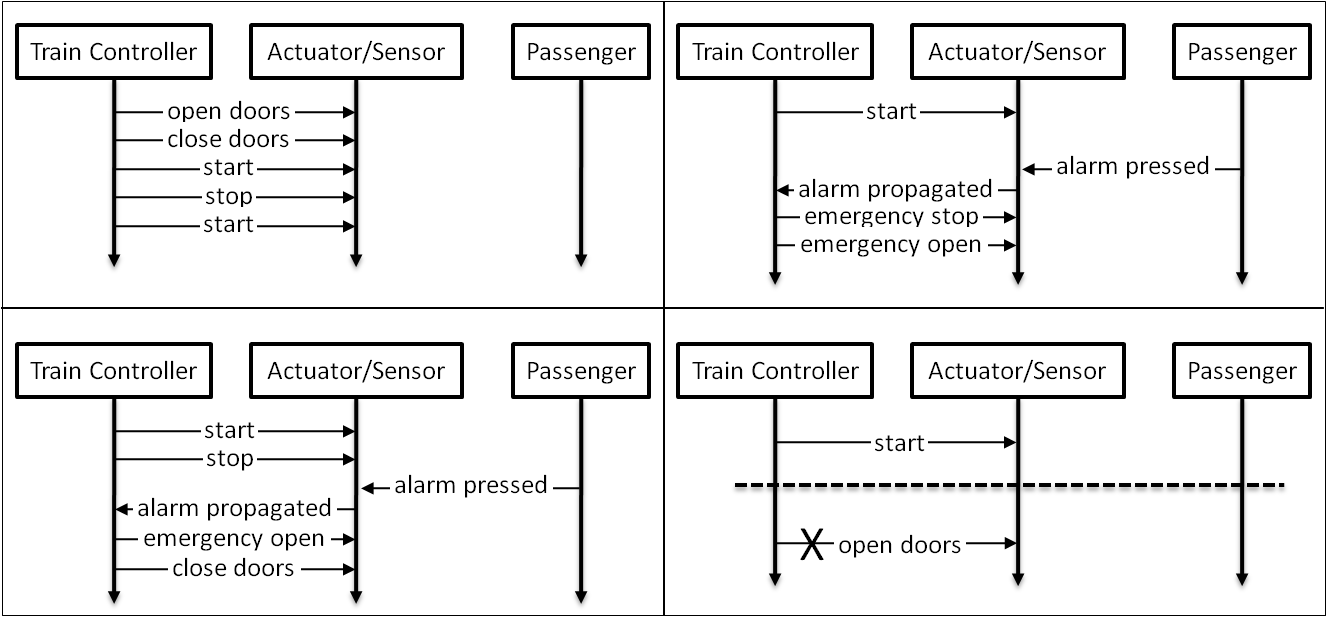
\includegraphics[trim=3mm 3mm 3mm 3mm, clip]{src/4-inductive/images/four-initial-scenarios}}
\caption{Initial positive and negative scenarios for a train system\label{Fig:init:scen}.}
\end{figure}


\item[ChooseStatePair] The candidate solution is refined by merging well- selected state pairs. The \texttt{ChooseStatePair} function determines which pairs to consider. It relies on the standard order $<$ on strings. Each state of the PTA can be labeled by its unique prefix from the initial state. Since prefixes can be sorted according to that order, the states can be ranked accordingly. For example, the PTA states in Fig.~\ref{Fig:algo:steps} are labeled by their rank according to this order. The algorithm considers states $q$ of the PTA in increasing order. The state pairs considered for merging only involve such state $q$ and any state $q'$ of lower rank. The $q'$ states are considered in increasing order as well. This particular ordering is specific to the original RPNI algorithm.

\item[Merge] The \texttt{Merge} function merges the two states $(q, q')$ selected in order to compute a quotient automaton, that is, to generalize the current set of positive behaviors. In the example of Fig.~\ref{Fig:algo:steps}, we assume that states 0, 1, and 2 were previously determined not to be compatible for merging (through negative scenarios initially submitted or generated scenarios that were rejected by the user). Merging a candidate state pair may produce a non-deterministic LTS. For example, after having merged $q = 3$ and $q' = 0$ in the upper part of Fig.~\ref{Fig:algo:steps}, two transitions labeled \texttt{start} from state 0 lead to states 2 and 6, respectively. In such a case, the \texttt{Merge} function merges states 2 and 6 and, recursively, any further pair of states that introduces non-determinism. 

We call \textsl{merging for determinization} this recursive operation of removing non-determinism. This operation guarantees that the current solution at any step is deterministic. It produces an automaton which may accept a more general language than the one it starts from. Therefore, it is not equivalent to the standard algorithm to transform a non deterministic automaton into a deterministic one accepting the same language~\cite{Hopcroft:1979}. Notably, the time complexity of merging for determinization is a linear function of the number of states of the automaton it starts from whereas the standard determinization algorithm is exponential in the worst case. Also, the resulting automaton is still part of the same inductive search space (see Section~\ref{subsection:gi-background-search-space}). 

\begin{figure}
\centering
\scalebox{.67}{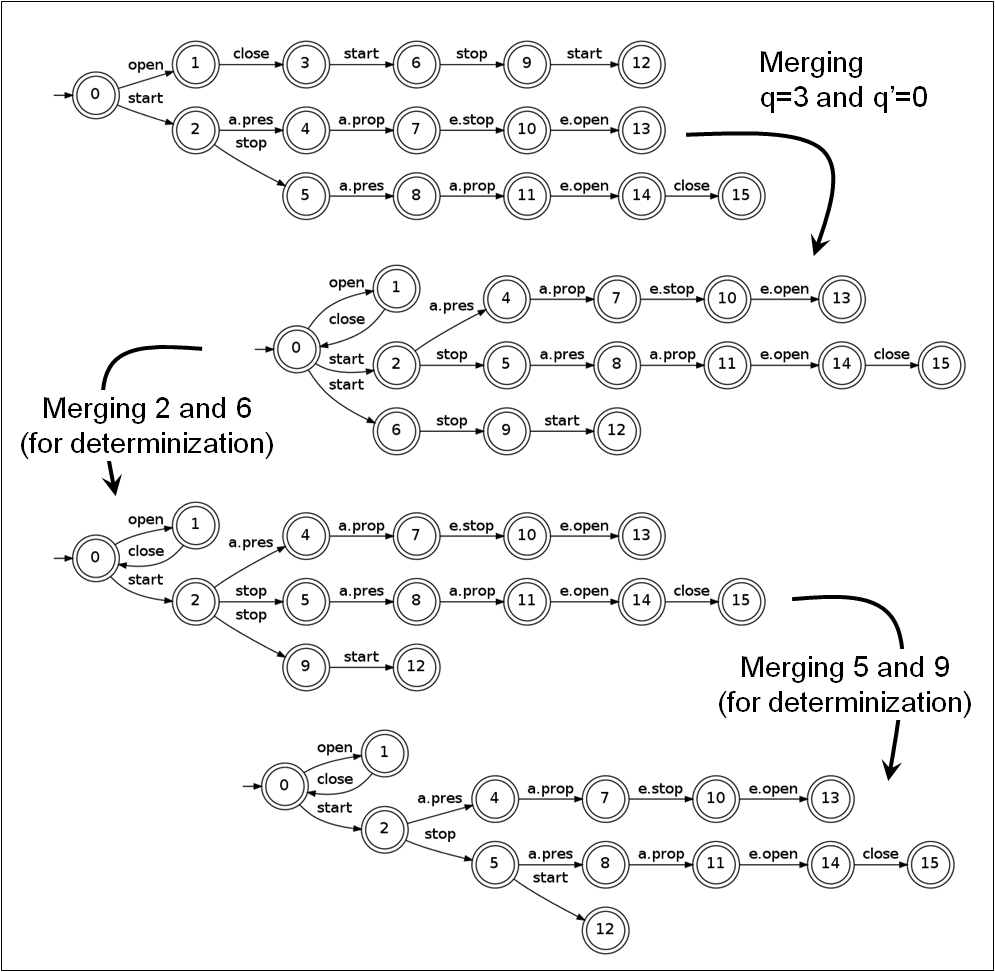
\includegraphics[trim=3mm 3mm 3mm 3mm, clip]{src/4-inductive/images/algo-steps}}
\caption{A typical induction step of the \textsc{QSM} algorithm\label{Fig:algo:steps}.}
\end{figure}

When two states are merged, the rank of the resulting state is defined as the lowest rank of the pair; in particular, the rank of the merged state when merging $q$ and $q'$ is defined as the rank of $q'$ by construction. If no compatible merging can be found between $q$ and any of its predecessor states according to $<$, state $q$ is said to be \textsl{consolidated}. In the example, states 0, 1, and 2 are consolidated.

\item[Consistent] The \texttt{Consistent} function checks whether the automaton $A_{new}$ correctly rejects all negative scenarios. As seen in the pseudo code, the quotient automaton is discarded by \textsc{QSM} when it is detected not to be consistent.

\end{description}

\subsection{Generating queries submitted to the end-user\label{QSM:query}}

This section describes how queries are generated in the \textsc{QSM} algorithm and how the answers provided by the end-user are processed.

\begin{description}

\item[GenerateQuery] When an intermediate solution is consistent with the available scenarios, new scenarios are generated for classification by the end-user as positive or negative. The aim is to avoid poor generalizations by enriching the possibly limited collection of initial scenarios. The notion of characteristic sample drives the identification of which new scenarios should be generated as queries. 

Recall from section~\ref{subsection:gi-background-rpni} that a sample is characteristic of a regular language $L$ if it contains enough positive and negative information. On the one hand, the required positive information is the set of short prefixes $Sp(L)$ which form the shortest histories leading to each state of the canonical automaton $A(L)$. This positive information must also include all elements of the kernel $N(L)$ which represents all system transitions, that is, all shortest histories followed by any admissible event. If such positive information is available, $A(L)$ can always be derived from the PTA by an appropriate set of merging operations. On the other hand, the negative traces provide the necessary information to make incompatible the merging of states which should be kept distinct. A negative trace which would exclude the merging of a state pair $(q, q')$ can be simply made of the shortest history leading to $q'$ followed by any continuation from state $q$ as detailed below.

Consider the current solution of our induction algorithm when a pair of states $(q, q')$ is selected for merging (line 5 in the pseudo code). By construction, $q'$ is always a consolidated state at this step of the algorithm; that is, $q'$ is considered to be in $Sp(L)$. State $q$ is always both the root of a tree and the child of a consolidated state. In other words, $q$ is situated at one letter of a consolidated state, that is, $q$ is considered to be in $N(L)$. States $q$ and $q'$ are compatible according to the available negative scenarios; they would be merged by the standard RPNI algorithm. The QSM extension will first confirm or infirm the compatibility of $q$ and $q'$ by generating scenarios to be classified by the end-user. The generated scenarios are constructed as follows.

\begin{figure}
\centering
\scalebox{.75}{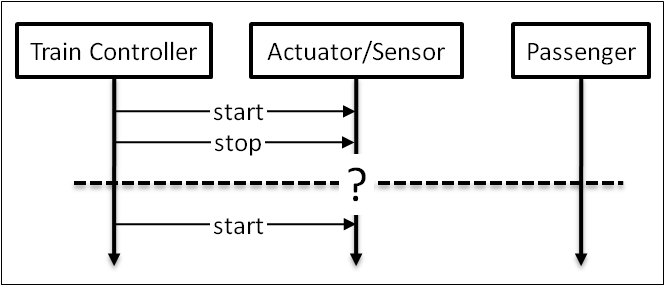
\includegraphics[trim=3mm 3mm 3mm 3mm, clip]{src/4-inductive/images/scenario-question}}
\caption{A new scenario to be classified by the end-user\label{Fig:generated:question}.}
\end{figure}

Let $A$ denote the current solution, $L(A)$ the language generated by $A$, and $A_{new}$ the quotient automaton computed by the \texttt{Merge} function at some given step. Let $x \in Sp(L)$ and $y \in N(L)$ denote the short prefixes of $q'$ and $q$ in A, respectively. Let $u \in L(A)/y$ denote a suffix of $q$ in $A$. 

A generated scenario is built from a system trace $xu$ such that $xu \in L(A_{new})\setminus L(A)$; it can be further decomposed as $xvw$ such that $xv \in L(A)$. The trace $xu$ is thus constructed as the short prefix of $q'$ concatenated with a suffix of $q$ in the current solution, provided the entire behavior is not yet accepted by $A$. Such system trace can be converted to MSC using the structural information provided by a context diagram \cite{Jackson:1995}. The scenario is made of two parts: the first part $xv$ is an already accepted behavior whereas the second part $w$ provides a continuation to be checked for acceptance by the end-user. When submitted to the end-user, the generated scenario can always be rephrased as a question: after having executed the first episode ($xv$), can the system continue with the second episode ($w$)? 

Consider the example in Fig.~\ref{Fig:algo:steps} with selected state pair $q=3, q'=0$. As $q'$ is the root of the PTA, its short prefix is the empty trace $\lambda$. The suffixes of $q$ here yield one generated question (Fig.~\ref{Fig:generated:question}), which can be rephrased as follows: when having started and stopped the train, can the controller restart it? One can see that the first episode of this scenario in Fig.~\ref{Fig:algo:steps} is already accepted by $A$ whereas the entire behavior is accepted in $A_{new}$.

\item[CheckWithEndUser] When a new scenario is generated, it is submitted as a query to the end-user. If the end-user classifies the $Query$ as positive, it is added to the collection of positive scenarios. This addition changes the search space as it extends $S^+$ and consequently the PTA. However, this extension is implicit as the new solution $A_{new}$ is, by construction, also a quotient automaton of this extended PTA. When the $Query$ is classified as negative the induction process is recursively started on the extended scenario collection.

\end{description}

The QSM algorithm has a polynomial time complexity in the size of the learning sample $\mathcal{L}^+(Sc)$, see \cite{Dupont:2008}. 

Moreover, when it receives a characteristic sample in the initial scenario collection it is guaranteed that no additional scenario can be classified as negative. It follows that QSM will not be called recursively anymore and stops by returning the target model. 

An experimental study of the actual sample size required to observe the convergence of \textsc{QSM} and the number of queries submitted to the end-user is detailed in Chapter~\ref{chapter:evaluation}.

\subsection{Reducing the number of queries; the blue-fringe optimization\label{BlueFringe}}

The order in which states are considered for merging by the \texttt{ChooseStatePair} function described in section~\ref{QSM:merging} follows from the implicit assumption that the current sample is characteristic. Consequently, two states are considered compatible for merging if there is no suffix to distinguish among them. This can lead to a significant number of scenarios being generated to the end-user when the initial sample is sparse and actually not characteristic for the target System LTS. 

To overcome this problem, one can use an optimized strategy known as Blue-Fringe~\cite{Lang:1998}. The difference lies in the way state pairs are considered for merging. The general idea is to early detect incompatible state pairs and, subsequently, first consider state pairs for which compatibility has the highest chance to be confirmed by the user through positive classification. The resulting ``please confirm'' interaction may also appear more appealing to the user.

\begin{figure}
\centering
\scalebox{.55}{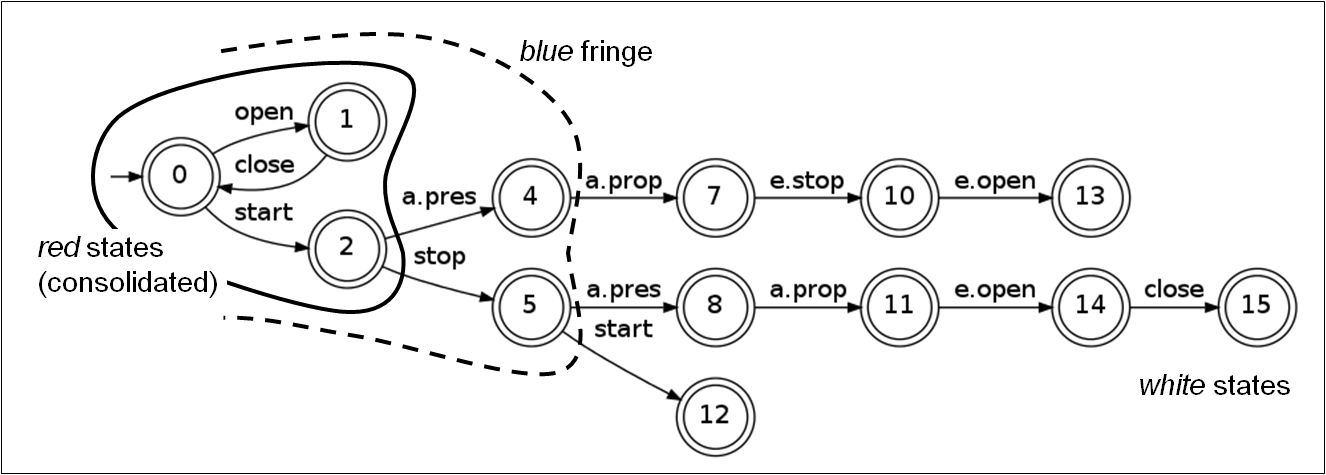
\includegraphics[trim=3mm 3mm 3mm 3mm, clip]{src/4-inductive/images/blue-fringe}}
\caption{Consolidated states (red) and states on the fringe (blue) in a temporary solution\label{Fig:BlueFringe}.}
\end{figure}

Fig.~\ref{Fig:BlueFringe} gives a typical example of a temporary solution produced by the original algorithm. Three state classes can be distinguished in this LTS. The red states are the consolidated ones (0, 1 and 2 in this example). Outgoing transitions from red states lead to blue states unless the latter have already been labeled as red. Blue states form the blue fringe (4 and 5 in this case). All other states are white states. 

The original \texttt{ChooseStatePair} function described in section~\ref{QSM:merging} considers the lowest-rank blue state first (state 4 here) for merge with the lowest-rank red state (0). When this choice leads to a compatible quotient automaton, generated scenarios are submitted to the end-user; in this case, a scenario equivalent to the trace \artifact{<alarm propagated, emergency stop, emergency open>}. The above strategy may lead to multiple queries being generated to avoid poor generalization. Moreover, such queries may be non-intuitive for the user, \textit{e.g.} the \artifact{alarm propagated} event is sent to the train controller without having been fired by the \artifact{alarm pressed} event to the sensor.

To select a state pair for merging, the Blue-Fringe strategy evaluates all (red, blue) state pairs first. The \texttt{ChooseStatePair} function now calls the \texttt{Merge} and \texttt{Compatible} functions before selecting the next state pair. If a blue state is found to be incompatible with all current red states, it is immediately promoted to red; the blue fringe is updated accordingly and the process of evaluating all (red, blue) pairs is iterated. When no blue state is found to be incompatible with red states, the most compatible (red, blue) pair is selected for merging. This is dictated by a scoring mechanism implemented in the \texttt{Compatible} function (see below).

For implementing the Blue-Fringe strategy, it is convenient to adapt \texttt{Initialize} so as to build an \emph{augmented} prefix tree acceptor. Such PTA captures the negative traces in $\mathcal{L}^-(Sc)$ in addition to the positive traces in $\mathcal{L}^+(Sc)$. States reached by a negative trace are tagged as error states; they are depicted in black, as in Fig. \ref{figure:augmented-pta}. 

The \texttt{Compatible} function is also updated to return a compatibility score instead of a boolean value. The score is defined as $-\infty$ when merging the current (red, blue) pair leads to merge an accepting state and an error state during merging for determinization\footnote{in the case of a prefix-closed language, non-error states are all accepting. Recall that this is not necessarily true for any regular language.}; this score indicates an incompatible merging. Otherwise, the compatibility score measures how many accepting states have been merged together. The (red, blue) pair with the highest compatibility score is considered first. The strategy can be further refined with a compatibility threshold $\alpha$ as additional input parameter. Two states are considered to be compatible if their compatibility score is above that threshold. This additional parameter controls the level of generalization since increasing $\alpha$ decreases the number of state pairs that are considered compatible for merging; it thus decreases the number of generated queries.

\begin{figure}\centering
\scalebox{.35}{\includegraphics*{src/4-inductive/images/augmented-pta}}
\caption{Augmented PTA for scenarios in Fig.~\ref{Fig:init:scen}\label{figure:augmented-pta}.}
\end{figure}

Experimental results about the effectiveness of using QSM with and without the Blue-Fringe strategy are detailed in Chapter~\ref{chapter:evaluation}.

\section{Using constraints for multi-view consistency\label{section:inductive-mutliview-consistency}}

The interactive QSM algorithm described in Section~\ref{section:lts-induction-from-mscs} provides a system LTS consistent with all available positive and negative scenarios. The Blue-Fringe strategy can also be applied to reduce the number of additional scenarios submitted to the end-user. The latter strategy relies on two equivalence classes partitioning the states of an augmented PTA. These classes correspond to the accepting states and the error states, respectively. All states belonging to the same class are not necessarily merged in the final solution; however, the \texttt{Compatible} function guarantees that only states belonging to the same class \emph{can} be merged.

This approach can be extended to achieve multi-view consistency by incorporating various sources of information. Such information refines the equivalence partition and further constrains the compatible merging operations. Injecting knowledge-based constraints has many advantages: 
\begin{itemize}
\item It ensures strong consistency of the system LTS with other views;
\item It reduces the number of scenario queries in the interactive setting;
\item It speeds up the search.
\end{itemize}

Section \ref{subsection:induction-pruning-with-domain-knowledge} shows how to incorporate domain knowledge such as fluent definitions. Section \ref{subsection:induction-pruning-with-goals} shows how goals can be used to constrain the generalization. 

The optimization techniques detailed hereafter are based on various equivalence relations over system states. The term \emph{equivalence relation} is used here in its usual mathematical sense, namely, a symmetric, reflexive, and transitive binary relation over states. The general principle underlying our techniques is the following:
\begin{quote}
\emph{Two states will be considered for merging if they agree according to all considered equivalence relations.}
\end{quote}

%%%%%

\subsection{Injecting domain knowledge\label{subsection:induction-pruning-with-domain-knowledge}}

The domain knowledge used to constrain state merging comes from multiple sources: 
\begin{itemize}
\item Fluent definitions;
\item Knowledge about components in the environment of the software-to-be;
\item Specifications of domain properties.
\end{itemize}
We discuss them successively.

%%

\subsubsection*{Propagating fluents}

Fluent definitions provide simple and easy-to-provide domain descriptions to constrain induction. For example, the definition
\begin{center}
fluent $DoorsClosed = \textless \{$close doors$\}, \newline
 \{$open doors, emergency open$\} \textgreater $ initially $true$ \\
\end{center}
describes train door states as being either closed ($DoorsClosed = true$) or open ($DoorsClosed = false$); it also states which event is responsible for which state change. 

Such descriptions can be effectively used to constrain the induction process so that the synthesized System LTS conforms to them. The idea is to decorate each state of the PTA with the value of every fluent. This can be done using a symbolic execution algorithm \cite{Damas:2006, Damas:2011} (see Section~\ref{section:background-fluents}).

The pruning rule for constraining the induction process is here to \emph{avoid merging inconsistent states} according to these decorations. 

The specific equivalence relation is thus the set of state pairs where both states have the same fluent value assignment. The decoration of the merged state is simply inherited from the states being merged.
\begin{quote}
\emph{Two states will be considered for merging if they have the same value for every fluent.}
\end{quote}

Fig.~\ref{dc-augmented-pta} shows the result of propagating the values of the fluent \emph{DoorsClosed} along the augmented PTA built from the scenarios described in Fig.~\ref{Fig:init:scen}.

\begin{figure}
\centering
\scalebox{.33}{\includegraphics*{src/4-inductive/images/dc-augmented-pta}}
\caption{Propagating fluents along the PTA to prune the inductive search space\label{dc-augmented-pta} (DC stands for \emph{DoorsClosed})}
\end{figure}

%%

\subsubsection*{Unfolding models of external components}

Quite often the components being modeled need to interact with other components in their environment - \textit{e.g.}, legacy components in a bigger existing system, foreign components in an open system, etc. In such cases the behavior of external components is generally known - typically, through some behavioral model \cite{Hall:2004}. External components are assumed here to be known by their LTS model. 

For example, Fig.~\ref{Fig.:alarm-sensor} shows the LTS for a legacy alarm sensor in our train system. When the alarm button is pressed by a passenger, this component propagates a corresponding signal to the train controller. 

\begin{figure}
\centering
\scalebox{.4}{\includegraphics*{src/4-inductive/images/alarm-sensor}}
\caption{LTS model for an alarm sensor\label{Fig.:alarm-sensor}.}
\end{figure}

A LTS model of an external component can constrain the induction process so that the synthesized system LTS conforms to it. The idea is to decorate the PTA with states of the external LTS by unfolding the latter onto the PTA. Such decoration is performed by jointly visiting the PTA and the external LTS; the latter synchronizes on shared events and remains in its current state on other events.

Fig.~\ref{Fig.:alarm-unfolded-pta} shows the result of unfolding the alarm sensor LTS from Fig.~\ref{Fig.:alarm-sensor} on the augmented PTA built from the scenarios described in Fig.~\ref{Fig:init:scen}. Each state of the PTA is labeled with the number of the corresponding state in the alarm sensor LTS. 

\begin{figure}
\centering
\scalebox{.35}{\includegraphics*{src/4-inductive/images/alarm-unfolded-pta}}
\caption{Unfolding the alarm sensor LTS onto the PTA\label{Fig.:alarm-unfolded-pta}.}
\end{figure}

The pruning rule for constraining the induction process is now to \emph{avoid merging states decorated with distinct states of the external component}. The specific equivalence relation used here is the set of states where both states have the same external LTS state. 

\begin{quote}
\emph{Two states will be considered for merging if they have the same external LTS state.}
\end{quote}

%%

\subsubsection*{Using declarative domain properties}

Descriptive statements and assumptions about the domain can be expressed declaratively in FLTL (see Section~\ref{section:background-goals}). For example, the physical law
\begin{align*}
\square(HighSpeed \rightarrow Moving)
\end{align*}
\noindent excludes all negative traces where the train is running at high speed while not moving. 

The technique for constraining induction through descriptive or prescriptive statements is the same; we discuss it hereafter.

%%%%%

\subsection{Injecting goals\label{subsection:induction-pruning-with-goals}}

For reasons discussed in Section \ref{section:background-goals}, we restrict our attention to goals and domain properties that can be formalized as pure FLTL safety properties. Remember that these properties refer to  ``\emph{something bad may never happen}''.

Consider the following goal requiring train doors to remain closed while the train is moving:
\begin{center}
\artifact{Maintain[DoorsClosed While Moving]} = $\square(Moving \rightarrow DoorsClosed)$
\end{center}

Fig.~\ref{Fig.:tester-automaton-inductive} shows the tester automaton for this property (cfr. Section \ref{subsection:background-property-and-tester-automata}). The accepting state of this tester captures all traces violating the safety property; any trace leading to it corresponds to an undesired system behavior. In particular, the trace \artifact{<start, open>} corresponds to the initial negative scenario in Fig.~\ref{Fig:init:scen}. As seen in Fig.~\ref{Fig.:tester-automaton-inductive}, the tester provides many more negative traces. Property testers can in fact provide potentially infinite classes of negative scenarios.

\begin{figure}
\centering
\scalebox{.35}{\includegraphics*{src/4-inductive/images/tester-automaton}}
\caption{Tester LTS for the goal \artifact{Maintain[DoorsClosed While Moving]}.\label{Fig.:tester-automaton-inductive}}
\end{figure}

The property tester is used to constrain the induction process in a way similar to an external component LTS. The PTA and the tester are traversed jointly in order to decorate each PTA state with the corresponding tester state. Fig.~\ref{Fig.:goal-unfolded-pta} shows the PTA decorated using the tester of Fig.~\ref{Fig.:tester-automaton-inductive}.

\begin{figure}
\centering
\scalebox{.35}{\includegraphics*{src/4-inductive/images/goal-unfolded-pta}}
\caption{Augmented PTA decorated using the tester automaton from Fig.~\ref{Fig.:tester-automaton-inductive}\label{Fig.:goal-unfolded-pta}.}
\end{figure}

The pruning rule for constraining the induction process is now to \emph{avoid merging states decorated with distinct states of the property tester}. The specific equivalence relation used here is the set of states where both states correspond to the same state of the property tester. 
\begin{quote}
\emph{Two states will be considered for merging if they have the same property tester state.}
\end{quote}

This pruning technique guarantees the consistency between the synthesized System LTS and the considered goals and domain properties. In other words, for every goal or domain property $G$ injected in the synthesis process, the following consistency condition holds (see Section \ref{subsection:background-goals-consistency}):
\begin{align*}
\mathcal{L}^-(G) \cap \mathcal{L}(System) &= \emptyset,
\end{align*}
where \emph{System} here denotes the synthesized system LTS and $\mathcal{L}^-(G)$ captures all traces violating $G$.

Note that the guarantee given by the above condition is weaker than the \emph{consistent system view} condition (\ref{relation:inductive-statement-negative}) in Section \ref{subsection:inductive-synthesis-statement}. The latter requires the consistency of the synthesized system $\system$ while the above condition only applies to the system LTS. As with implied negative scenarios, a goal could be satisfied by the synthesized System LTS while being violated by the real distributed system. This issue is further discussed in Section \ref{section:inductive-discussion}.

\subsection{Discussion\label{subsection:qsm-constraints-implementation-notes}}

The equivalence relations considered in the previous sections are all invariant under state merging. In other words, a state derived by merging some states simply inherits their relation. This allows each relation to be computed only once on the initial PTA; the results of such pre-processing are kept as annotations on PTA states. 

Our implementation reuses the decoration algorithm from \cite{Damas:2006} to propagate fluent values on the PTA (see Section~\ref{subsection:fluents-along-multiple-traces}). Its generalization in~\cite{Damas:2011} may be used as an effective mean to unfold models of legacy components and tester automata on the PTA without additional developments.

The principle for constraining state merging through equivalence relations first appeared in~\cite{Coste:1998, Coste:2004}. It can be further instantiated to other equivalence relations not considered here. In particular, it is \emph{not} limited to relations that are invariant under state merging.

As an illustrative example, consider the following generalization of the way fluent values are used to constrain the induction process. We know from Section~\ref{subsection:fluents-along-multiple-traces} that the states of any LTS can be annotated with invariants defined on fluents. Let $inv$ denote the function mapping each PTA state to its state invariant; let also denote by \emph{Dom} a domain property that must be met in every state of the system LTS. Consider the following pruning rule:
\begin{quote}
\emph{Two states $q$ and $q'$ will be considered for merging if $inv(q) \wedge inv(q') \models \mbox{Dom}$}
\end{quote}

The equivalence relation here is the set of state pairs whose conjunction of invariants satisfies the domain property. This equivalence relation is \emph{not} invariant under state merging. The merging constraint can however be enforced; to achieve this, the compound state resulting from merging $q$ and $q'$ has to be annotated by the conjunction of their state invariants; this new invariant is then used in subsequent state merging.

In the general case of DFA induction\footnote{that is, in contrast to LTS induction}, a similar mechanism is needed to implement the Blue-fringe optimization with an augmented PTA. In that case, an error state may be merged with a non accepting state provided the result is not merged later with an accepting one. That is, the relation capturing the equivalence of states in terms of their continations is not invariant under state merging.

\section{LTS synthesis from high-level MSCs\label{section:inductive-from-hMSC}}

The previous sections have shown how system behaviors specified in collections of MSC scenarios can be first generalized as a System LTS, then decomposed as a set of agent LTSs. The technique supports the incremental enrichment of an initial scenario collection through scenario queries. It also takes other models into account, such as goals, so as to preserve multi-view consistency. Behavior generalization, incremental synthesis and multi-view consistency are the three main requirements identified in Section \ref{subsection:inductive-synthesis-requirements}. 

Coupled with other synthesis techniques such as goal mining from scenarios\footnote{whose simplest form consists in asking ``why'' when facing with a negative scenario.} \cite{Damas:2006}, interactive LTS induction is really effective; starting from a small initial scenario collection, richer system models can be synthesized in only a few iterations. Chapters~\ref{chapter:evaluation} and \ref{chapter:tool-support} illustrate this claim with evaluations and overview of the tool support.

However, for any non-toy system, a large scenario collection might become unmanageable. Among others, consistency of the collection might be difficult to guarantee without costly refactoring on scenarios. One reason is that all scenarios of a collection are required to start in the same system state; this usually implies a lot of redundancy in system descriptions.

One way to tackle this problem is to use high-level message sequence charts (hMSCs) for structuring scenario descriptions. As detailed in Section \ref{subsection:background-hmsc}, hMSCs are directed graphs where each node refers to a MSC or a finer grained hMSC (see Fig.~\ref{image:train-hmsc}). Scenarios can then be structured by introducing alternatives, sequences and loops.

Having a structured form of scenario \emph{helps} specifying a large system with scenarios; it does not \emph{solves} the problem of achieving a complete and consistent view of agent behaviors:
\begin{itemize}
\item capturing all possible interleavings of a distributed system proves difficult with scenarios; a hMSC is therefore hardly complete in practice,
\item complementary features of a system deserve being specified in complementary models; in addition to using multiple system views, having system behaviors specified in more than one hMSC makes sense.
\end{itemize}

Having a synthesis technique to merge and to generalize behaviors described in hMSCs seems a convenient extension to the synthesis technique described so far. For this, the LTS synthesis statement is first revisited in Section~\ref{subsection:hmsc-induction-problem-revisited}. The inductive algorithm is then adapted in Section \ref{subsection:hmsc-induction-algo-adaptation}.

\subsection{Revisiting the LTS synthesis statement\label{subsection:hmsc-induction-problem-revisited}}

Merging multiple hMSCs $H_1,\ldots,H_n$ with respect to trace behaviors simply amounts to compute the union of their respective languages. This is equivalent to building a new hMSC $H$ reaching the finer-grained $H_1,\ldots,H_n$ from its initial state. Additional positive scenarios $S^+_1,\ldots,S^+_n$, typically coming from scenario queries, could be integrated in a similar way. This is illustrated in Fig.~\ref{figure:multiple-hmscs}.

\begin{figure}\centering
\scalebox{.70}{
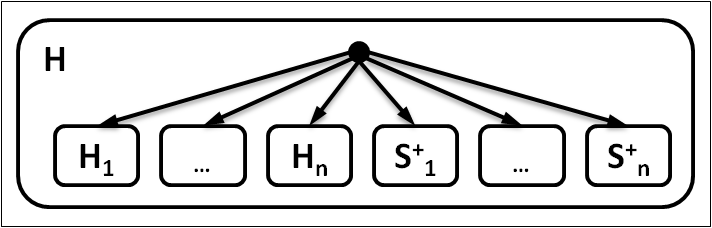
\includegraphics[trim=3mm 3mm 3mm 3mm, clip]{src/4-inductive/images/multiple-hmscs}}
\caption{Merging multiple hMSCs amounts to builds a new one that reaches finer-grained hMSCs from its initial state.\label{figure:multiple-hmscs}} 
\end{figure}

However, a hMSC only permits specifying positive behaviors. As explained in previous sections, negative information is needed to avoid poor generalizations. Negative scenarios, fluents, goals, etc. all provide a source of negative knowledge that can be used to constraint the induction process. The algorithmic adaptations considered later stay compatible with the constraint mechanism based on equivalence relations on system states.

Without loss of generality therefore, we will assume that behaviors are specified through one hMSC only, complemented with a scenario collection. The latter contains negative scenarios and answers to scenario queries. Under these assumptions, the LTS synthesis statement is restated as follows: 

\begin{quote}
\underline{Given}~a hMSC $H$ and a scenario collection $Sc = (S^+,S^-)$ consistent with each other
\begin{align*}
[\mathcal{L}^+(Sc) \cup \mathcal{L}(H)] \cap \mathcal{L}^-(Sc) &= \emptyset
\end{align*}
\underline{Synthesize}~the system as a composition of agent LTSs
\begin{align*}
System = (Ag_1 \parallel \ldots \parallel Ag_n)
\end{align*}
\underline{Such that}~$H$, $Sc$ and $System$ are consistent.
\end{quote}

The hMSC trace semantics is left open in the formulation above. In other words, one has to decide which set of behaviors does $\mathcal{L}(H)$ denote. We recall below the relations between the three hMSC languages covered in Section \ref{subsection:background-hmsc}: 
\begin{align}
\mathcal{L}_{strong}(H) \subseteq \mathcal{L}_{weak}(H) &\subseteq \mathcal{L}_{arch}(H)
\end{align}

$\mathcal{L}_{strong}(H)$ denotes the set of system behaviors with strong sequential composition of hMSC nodes and total event ordering inside MSCs. It is the simplest and most intuitive model for stakeholders involved in early phases of system design. However, it supposes an implicit synchronization scheme used by the agents that is usually not available in real distributed systems. $\mathcal{L}_{arch}(H)$ is the most realistic for such systems, as it captures all possible interleavings of agent behaviors. $\mathcal{L}_{weak}(H)$ is mainly used for explaining and detecting implied scenarios in hMSC specifications \cite{Uchitel:2003}; it is also the hardest to compute.

Making a choice of semantics is required for generalizing behaviors because inductive synthesis takes a set of traces as input. The chosen semantics must of course fit domain assumptions. From an algorithmic point of view however, the three hMSC languages above require the same adaptations of the inductive process, as explained in the next sections.

\subsection{Generalizing high-level MSC languages\label{subsection:hmsc-induction-algo-adaptation}}

Recall that learning a regular language $L$ aims at generalizing a positive sample $S_+$ under the control of a negative sample $S_-$ such that the following relation of language inclusions holds:
\begin{align}
S_+~~\subseteq~~L~~\subseteq~~\Sigma^*\setminus S_-
\end{align}

LTS synthesis from a scenario collection $Sc$ reduces to grammar induction because the sets $\mathcal{L}^+(Sc)$ and $\mathcal{L}^-(Sc)$ are valid positive and negative samples, respectively (see Section \ref{subsection:inductive-lts-synthesis-reduction}). In particular, they denote \emph{finite} sets of traces.

When considering the generalization of hMSC behaviors, the sets of positive and negative traces are $\mathcal{L}^+(Sc) \cup \mathcal{L}(H)$ and $\mathcal{L}^-(Sc)$, respectively. The positive set is no longer a sample because $\mathcal{L}(H)$ might contain an infinite number of traces. Therefore, the current problem statement no longer fits exactly in the identification in the limit framework presented in Section \ref{section:inductive-background}. 

From a theoretical point of view, it means that generalizing hMSC languages is a different problem than generalizing MSC languages; therefore, further study would be needed to re-state the convergence criteria and the notion of characteristic sample in particular. From an algorithmic point of view, however, only a few adaptations of RPNI and QSM are required. They are explained in the next section.

\subsection{The Automaton State Merging algorithm\label{subsection:automaton-state-merging}}

The algorithm to generalize behaviors specified in a hMSC is given in Algorithm~\ref{ASM}, called Automaton State Merging (ASM). It is very similar to QSM, given in Section~\ref{section:lts-induction-from-mscs}, except that the interactive feature is ommited here (we discuss it later). QSM itself being an interactive extension to RPNI, Algorithm~\ref{ASM} is almost RPNI itself which might appear suprising at first glance.

\begin{algorithm}
{
\vspace{0.2cm}
\KwIn{A high-level MSC $H$ and a scenario collection $Sc = (S_+, S_-)$}
\KwOut{A System LTS, consistent with both $H$ and $Sc$}

$A \leftarrow $ {\tt Initialize($H$, $Sc$)}\\
\While{$(q,q') \leftarrow $ {\tt ChooseStatePair($A$)}}{
$A_{new} \leftarrow$ {\tt Merge$(A,q,q')$}\\
\If{{\tt Consistent$(A_{new}, S_-)$}}{
 $A \leftarrow A_{new}$
}
}
\Return{$A$}}
\vspace{0.2cm}
\caption{\textsc{ASM}, a state-merging algorithm from high-level Message Sequence Charts\label{ASM}}
\end{algorithm}

The main difference between RPNI and QSM on one side and ASM on the other side is the initial automaton solution built by \texttt{Initialize}. RPNI and QSM initially convert the input \emph{sample} as a PTA, hence a tree, whereas ASM converts the input \emph{language} of the hMSC as a DFA, hence an graph. The main loop of the ASM algorithm can then be seen as generalizing any regular language, under the control of a negative sample; hence the ``Automaton State Merging'' name. A few adaptations are however required to the different functions of the algorithm: 

\begin{description}

\item[Initialize] This function is adapted to return a DFA instead of a PTA. On one side, the positive traces from the hMSC may be captured through a LTS as discussed in Section \ref{subsection:background-hmsc}, provided a choice of hMSC semantics. On the other side, the scenario collection can be captured through a PTA. These two automata can be merged through standard algorithms for capturing the union of regular languages \cite{Hopcroft:1979}. 

In order to use the Blue-Fringe heuristic (see below), the obtained DFA may be augmented with error states encoding the negative sample given by $S_-$. 

\item[ChooseStatePair] In order to preserve the merging order used by RPNI, this function must be slightly adapted. The idea is to pre-compute the natural order among the states of the initial DFA solution. A breadth first search is used and each of them is numbered when encountered. 

Not that the Blue-Fringe strategy does not require special support. The distinction between red and blue states does not rely on any assumption about the initial solution being a tree; in particular, the fact that a fringe state is the root of a tree in RPNI and QSM is incidental (see \texttt{Merge} below).

\item[Merge] The merging for determinization process is often implemented assuming a tree invariant property. This property states that, when considering two states to be merged, at least one of them is the root of a tree. Such a property holds for RPNI and QSM, even when the Blue-Fringe optimization is used. It is a sufficient condition for the determinization process to be finite. 

Even though it is convenient, the tree invariant property is not required, as explained in \cite{Lambeau:2008}. The main merging loop and the \texttt{Merge} function can be implemented without the tree invariant property because the recursive determinization process stops naturally on the first DFA encountered. This observation allows one to start from an arbitrary DFA and, as soon as non-determinism occurs, to reduce it. 
%Fig.~\ref{figure:merging-for-determ-on-dfa} gives an example of such a recursive operation.

\end{description}

The interactive feature of QSM could be easily adapted and plugged to ASM. It consist in replaincing the main loop ASM by the one of QSM (see Algorithm~\ref{QSM} in Section~\ref{section:lts-induction-from-mscs}). In the latter, the \texttt{GenerateQuery} function must be adapted as follows:

\begin{description}

\item[GenerateQuery] The generation of scenario queries relies on the tree invariant property mentioned above. When merging a state pair $(q,q')$, a scenario query is built with the shortest trace leading to $q$ concatenated with the suffixes of $q'$. When $q'$ is the root of a tree, generating a finite scenario is straightforward.

If the tree invariant property no longer holds, the \texttt{GenerateQuery} function must be extended with a procedure for extracting finite suffixes from $q'$. This does not introduce any technical issues; for example, pre-computing a spanning tree on the initial DFA would associate finite suffixes to each of its state. However, what forms a ``good'' suffix for convergence and scenario classification by end-users is an open question. As the adapted algorithm no longer fits in the identification in the limit framework, the notion of a characteristic sample would need to be adapted. 

\end{description}

%\begin{figure}\centering
%\scalebox{.34}{
%\includegraphics*{src/4-inductive/images/merging-for-determ-on-dfa}}
%\caption{Recursive determinization process. States \{3\} and \{0\} of an arbitrary DFA are merged, which causes a non-determinism on letter $b$ from state \{0,3\}. The destination states \{2\} and \{4\} are subsequently merged to reduce the non-determinism.\label{figure:merging-for-determ-on-dfa}} 
%\end{figure}

From a grammar induction point of view, the ASM algorithm can be seen as generalizing any positive regular language $\mathcal{L}^+$ under the control of a negative sample $S_-$. As such, RPNI is thus a special case where the positive language forms a sample $S_+$, that is a finite set of strings.

Interrestingly, the constraint mechanism from Section~\ref{section:inductive-mutliview-consistency} to prune the induction search space and guarantee multi-view consistency can still be used with ASM. Indeed, the partitionning of PTA states according to equivalence relations extracted from domain knowledge can be performed on the input DFA returned by \texttt{Initialize}, \emph{mutatis mutandis}. 

In particular, goals and domain properties can still be used to prune the induction search space, as explained in Section~\ref{subsection:induction-pruning-with-goals}. As goals actually capture negative languages through their tester automaton, this amounts to consider yet another generalization of ASM to generalize a positive language $\mathcal{L}^+$ under the control of a negative one $\mathcal{L}^-$. This generalization is called ASM$^*$ and briefly discussed in \cite{Lambeau:2008}.



\section{Correctness\label{section:inductive-correctness}}

Proving the correctness of our synthesis approach amounts to show that the synthesized system is consistent with both the scenarios and all domain knowledge taken in input. We discuss proof arguments for the different algorithm settings, starting with the simplest case of RPNI-based synthesis and gradually integrating features such as scenario questions and injection of domain knowledge.

\begin{figure}\centering
\scalebox{.65}{
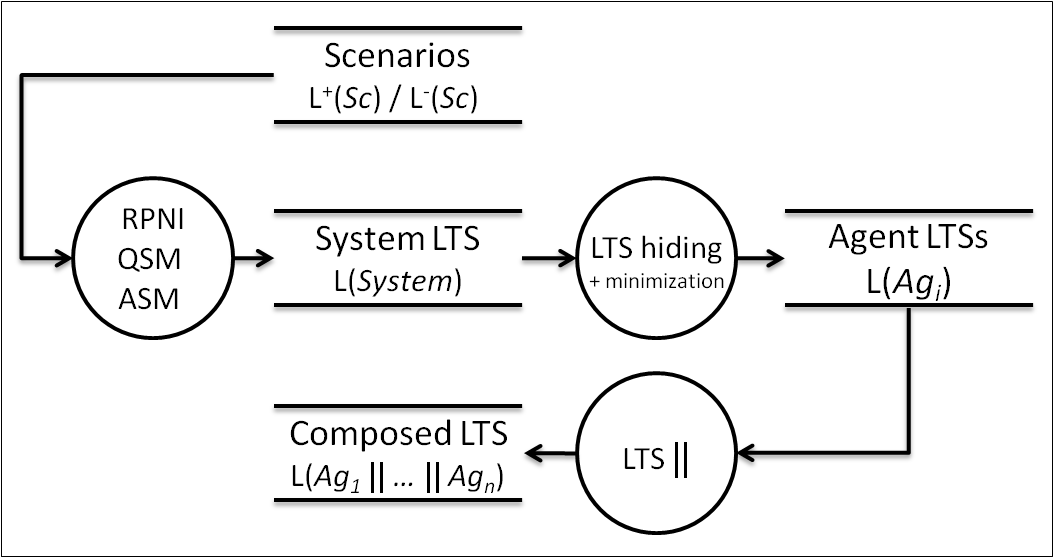
\includegraphics[trim=3mm 3mm 3mm 3mm, clip]{src/4-inductive/images/synthesis-flow-model}}
\caption{Inductive synthesis steps and products.\label{figure:synthesis-flow-model}} 
\end{figure}

Fig.~\ref{figure:synthesis-flow-model} summarizes our approach by showing used algorithms together with their input/output in terms of behavior models and associated languages. 
\begin{itemize}
\item From scenarios, a system LTS is inferred using either RPNI, QSM or ASM. 
\item LTS hiding and minimization is then used to obtain a canonical state machine for each agent. 
\item From the system view point, the result of our synthesis approach is precisely captured by the composition of those state machines.
\end{itemize}

In this figure and in the following discussions,
\begin{itemize}
\item $Sc = (S^+,S^-)$ denotes the input scenario collection; its positive and negative languages are denoted by $\mathcal{L}^+(Sc)$ and $\mathcal{L}^-(Sc)$, respectively.
\item $\mathcal{L}(\me{System})$ denotes the language captured by the inferred system LTS.
\item $\mathcal{L}(Ag)$ denotes the language of an arbitrary agent $Ag$, as captured by its LTS state machine.
\item $\mathcal{L}(\agentscomposed)$ denotes the language captured by the LTS resulting of the composition of individual agent LTSs.
\end{itemize}

We first restrict our attention to the simplest, non-interactive, RPNI approach. Remember from Section~\ref{subsection:inductive-synthesis-statement} that the specification on our approach requires three conditions to hold on synthesized state machines:
\begin{itemize}
\item The \emph{structural consistency} condition requires input scenarios and synthesized agent state machines to agree on the respective agent interfaces.
\item The \emph{consistent agent view} condition requires each synthesized agent state machine to cover the positive behaviors along the corresponding timeline in the input scenarios.
\begin{align}
\mathcal{L}^+(Sc_{\downarrow Ag}) \subseteq \mathcal{L}(Ag)\mbox{~for each agent $Ag$}\label{proof:consistent-agent-view}
\end{align}
where $Sc_{\downarrow Ag}$ denotes the positive behaviors along $Ag$'s timeline in a scenario collection $Sc = (S^+, S^-)$:
\begin{align}
\mathcal{L}^+(Sc_{\downarrow Ag}) = \bigcup_{P \in S^+} \mathcal{L}(P_{\downarrow Ag})~~\cup~~\bigcup_{N \in S^{-}} \mathcal{L}^{+}(N_{\downarrow Ag})\label{proof:lemma-sc-projection}
\end{align}

This is a a slight generalization of the concept of agent traces along a single scenario timeline $M_{\downarrow Ag}$, introduced in Section~\ref{section:background-scenarios}. Observe that it takes both positive and negative scenarios into account.
\item The \emph{consistent system view} requires the system to cover all positive scenarios and reject all negative ones. 
\begin{align}
&\mathcal{L}^+(Sc) \subseteq \mathcal{L}(\agentscomposed)\label{proof:consistent-system-view-1}\\
&\mathcal{L}^-(Sc) \cap      \mathcal{L}(\agentscomposed) = \emptyset\label{proof:consistent-system-view-2}
\end{align}
\end{itemize}

Section~\ref{subsection:system-lts-consistency} briefly discusses the consistency of the inferred system LTS with the scenarios. This result is then used in Section~\ref{subsection:consistent-agent-view} to show that the decomposition step meets the ``structural consistency'' and the ``consistent agent view'' conditions. The ``consistent system view'' condition is further discussed in Section~\ref{subsection:consistent-system-view}. The discussion is pursued in the presence of scenario questions in Section~\ref{subsection:proof-with-scenario-questions} and with the injection of domain knowledge in Section~\ref{subsection:proof-with-domain-knowledge}. Section~\ref{subsection:correctness-of-asm} closes this section with a discussion about the correctness of ASM.

%%%

\subsection{Consistency of the system LTS\label{subsection:system-lts-consistency}}

This section demonstrates that RPNI yields a system LTS consistent with the input scenario collection. The pseudo code given in Algo.~\ref{QSM} is used, ignoring the scenario questions (lines 5 to 10).

\begin{theorem}
\label{theorem:system-lts-consistency-with-sc}
The system LTS synthesized by RPNI covers all positive scenarios and rejects all negative ones.
\begin{align*}
&\mathcal{L}^+(Sc) \subseteq \mathcal{L}(System)\\
&\mathcal{L}^-(Sc) \cap      \mathcal{L}(System) = \emptyset
\end{align*}

\begin{proof}
This theorem is proven by induction using the following invariant:
\begin{align}
&\mathcal{L}^+(Sc) \subseteq \mathcal{L}(A_i)\label{inv:system-lts-consistency-with-sc-1}\\
&\mathcal{L}^-(Sc) \cap      \mathcal{L}(A_i) = \emptyset\label{inv:system-lts-consistency-with-sc-2}
\end{align}

\begin{description}
\item[Base:] $A_0$ denotes the PTA returned by \emph{Initialize}.

The PTA is the largest DFA accepting the positive language; a precondition states that input scenarios are consistent. Therefore the following conditions hold, entailing the invariant:
\begin{align}
&\mathcal{L}^+(Sc) =    \mathcal{L}(A_0)\\
&\mathcal{L}^-(Sc) \cap \mathcal{L}(A_0) = \emptyset
\end{align}

\item[Inductive step:] $A_i$ is the quotient automaton denoting the current solution at step $i$.

From a solution $A_i$, the next solution $A_{i+1}$ is computed by the \emph{Merge} function (see line 3 in Algo.~\ref{QSM}). The latter computes a quotient automaton. Definition~\ref{definition:quotient-automaton} guarantees that such quotient automaton may only generalize the language of $A_i$. As the condition~(\ref{inv:system-lts-consistency-with-sc-1}) holds for $A_i$, the following condition holds as well:
\begin{align*}
&\mathcal{L}^+(Sc) \subseteq \mathcal{L}(A_i) \subseteq \mathcal{L}(A_{i+1})
\end{align*}

On an other hand, quotient automata are only kept as next solution if consistent with the negative scenarios (see lines 4 and 11). Therefore, the following condition holds when such solution is kept (line 11):
\begin{align*}
&\mathcal{L}^-(Sc) \cap \mathcal{L}(A_{i+1}) = \emptyset
\end{align*}

\end{description}
\end{proof}
\end{theorem}

A detailed proof of the convergence of RPNI towards the canonical target automaton when it receives a characteristic sample can be found in~\cite{Oncina:1993} in the more general case of transducer learning.

%%%

\subsection{Structural consistency and consistent agent view\label{subsection:consistent-agent-view}}

Given the consistency of the system LTS with the positive and negative scenarios, the decomposition step guarantees that the \emph{structural consistency} and the \emph{consistent agent view} both hold.

Structural consistency only requires the LTS hiding step to make use of adequate agent alphabets, as induced from the scenarios themselves or given by a (consistent) structural model. We do not discuss it further. 

For each agent $Ag$, the ``consistent agent view'' condition (\ref{proof:consistent-agent-view}) can be derived from (\ref{proof:consistent-system-view-1}) using the following properties and definitions:
\begin{align}
&\mathcal{L}(X) \subseteq \mathcal{L}(Y) \implies \mathcal{L}(X \setminus I) \subseteq \mathcal{L}(Y \setminus I) \label{proof-agent-consistency-1}\\
&\mathcal{L}^+(Sc_{\downarrow Ag}) = \mathcal{L}^+(Sc \setminus \Sigma_{Ag}^c)\label{proof-agent-consistency-2}\\
&\mathcal{L}(Ag) = \mathcal{L}(System \setminus \Sigma_{Ag}^c)\label{proof-agent-consistency-3}
\end{align}
where $\Sigma_{Ag}^c$ denotes the set of all system events excluding those of $Ag$'s interface.
\begin{itemize}
\item (\ref{proof-agent-consistency-1}) states that behavior inclusion is preserved under LTS hiding; this property follows from material in Section~\ref{subsection:lts-hiding}. 
\item (\ref{proof-agent-consistency-2}) rewrites the left term of (\ref{proof:consistent-agent-view}) in terms of hiding of scenario behaviors\footnote{using an abuse of notation as the hiding operator is defined on LTS, not on scenarios collections.}. It can be derived from (\ref{proof:lemma-sc-projection}) and the definition of $M_{\downarrow Ag}$ (see Section~\ref{subsection:background-positive-scenarios}). 
\item (\ref{proof-agent-consistency-3}) follows from the definition (\ref{definition:decomposition-step}) of decomposition step itself (see Section~\ref{subsection:inductive-synthesis-approach}). 
\end{itemize}

From Theorem~\ref{theorem:system-lts-consistency-with-sc} ensuring the consistency of the system LTS with input scenarios, the following condition is established thanks to (\ref{proof-agent-consistency-1})
\begin{align}
&\mathcal{L}^+(Sc \setminus \Sigma_{Ag}^c) \subseteq \mathcal{L}(System \setminus \Sigma_{Ag}^c)\label{proof:consistent-agent-view-milestone}
\end{align}

The ``consistent agent view'' condition (\ref{proof:consistent-agent-view}) is established by substituing the right terms of (\ref{proof-agent-consistency-2}) and (\ref{proof-agent-consistency-3}) in (\ref{proof:consistent-agent-view-milestone}).

%%%

\subsection{Consistent system view: the problem of implied scenarios\label{subsection:consistent-system-view}}

This section discusses the correctness of the ``consistent system view'' condition. The conditions related to the positive and negative scenarios are discussed in turn.

\begin{theorem}
The synthesized system covers all positive scenarios.
\begin{align*}
&\mathcal{L}^+(Sc) \subseteq \mathcal{L}(\agentscomposed)
\end{align*}

\begin{proof}
This condition results from two main properties of our approach:
\begin{itemize}
\item The synthesized system LTS covers all positive scenario behaviors, as guaranteed by Theorem~\ref{theorem:system-lts-consistency-with-sc}.
\begin{align*}
&\mathcal{L}^+(Sc) \subseteq \mathcal{L}(System)
\end{align*}
\item Projecting the system LTS on agent alphabets and recomposing their LTS afterwards does not restrict behaviors:
\begin{align*}
&\mathcal{L}(\mbox{System}) \subseteq \mathcal{L}(\agentscomposed)
\end{align*}
This latter condition can be derived from the definition of agent languages (\ref{proof-agent-consistency-3}) and properties of LTS hiding and composition operators (see Section~\ref{section:background-state-machines}).
\end{itemize} 

\end{proof}
\end{theorem}

\begin{theorem}
The synthesized system excludes all negatives scenarios.
\begin{align*}
&\mathcal{L}^-(Sc) \cap \mathcal{L}(\agentscomposed) = \emptyset
\end{align*}
\end{theorem}

This theorem would require the composed system to exclude all negative scenarios. Due to the potential presence of implied scenarios, our approach only guarantees the weaker condition given by Theorem~\ref{theorem:system-lts-consistency-with-sc}, namely,
\begin{align*}
&\mathcal{L}^-(Sc) \cap \mathcal{L}(\mbox{System}) = \emptyset
\end{align*}

In other words, the induction algorithm ensures that the system LTS excludes all negative scenarios. This property can however be lost after the decomposition and recomposition steps.

The reason has to be found in the possible occurence of so-called \emph{implied scenarios}. Remember from Section~\ref{subsection:background-hmsc} that implied scenarios may appear when a system is specified globally while implemented component-wise ~\cite{Alur:2000, Uchitel:2004}. In our case, the set of implied scenarios is precisely defined as:
\begin{align*}
\mathcal{L}(\agentscomposed) \setminus \mathcal{L}(\mbox{System})
\end{align*}

When this language is not empty, implied scenarios denote system behaviors that the system LTS does not accept but which are exhibited by the composition of agent LTSs. Implied scenarios appear when, once distributed, the agents lack monitoring abilities to restrict their behavior so as to precisely match the system LTS.

Not all implied scenarios are problematic in practice. In particular, it might happen that all implied scenarios denote desired system behaviors. In that case, the presence of implied scenarios is not problematic and may be seen as the result of a second generalization step due to the decomposition and recomposition of agent LTS. This second generalization step proves useful as it weakens the necessity of having a pure structurally complete scenario collection in the first place.

Negative implied scenarios, that is, counterexamples of desired behaviors, are more problematic. In particular, a behavior trace $t$ could be such that the following conditions hold:
\begin{align}
&t \in \mathcal{L}^-(Sc)\label{implied-1}\\
&t \notin \mathcal{L}(\mbox{System})\label{implied-2}\\
&t \in \mathcal{L}(\agentscomposed)\label{implied-3}
\end{align}
that is, (\ref{implied-1}) $t$ denotes a system behavior explicitly rejected through a negative scenario; it might be a question answered negatively; (\ref{implied-2}) $t$ is correctly rejected by the system LTS; (\ref{implied-3}) $t$ is still be exhibited by the composed system.

In such case, observe the ``consistent system view'' condition is not met as (\ref{proof:consistent-system-view-2}) does not hold. As with other scenario approaches, e.g. \cite{Alur:2000, Uchitel:2004}, our synthesis technique fails to guarantee a consistent system view between scenarios and state machines in presence of negative implied scenarios.

In order to detect such situations, the technique from \cite{Uchitel:2004} could be adapted to enumerate implied scenarios and submit them as additional scenario questions to the user (see Section~\ref{section:related-for-analysis-3}). 

Note that, fixing implied scenario problems requires rethinking the system decomposition into agents and/or refactoring their interfaces. In other words, the root cause of implied scenarios problems has to be found in the structural decomposition of the system, not in the particular technique used to infer state machines from scenarios. 

%%%

\subsection{Correctness in the presence of scenario questions\label{subsection:proof-with-scenario-questions}}

The specification of QSM has been strengthened in Section~\ref{section:lts-induction-from-mscs}. This strengthening required the synthesized system to be consistent with all scenario questions in addition to the initial scenario collection. 

Provided a consistent system LTS is inferred with QSM, the correctness arguments for the \emph{structural consistency} and \emph{consistent agent view} conditions remain unchanged. The discussion about implied scenarios also takes place here. Therefore, we only prove the consistency of the system LTS induced by QSM when scenario questions are taken into account.

\begin{theorem}
The system LTS inferred by QSM is consistent with the scenario collection extended with the answers to all scenario questions.

\begin{proof}
This theorem is proven by induction (cfr. Algo.~\ref{QSM}):
\begin{description}
\item[Base:] The base case captures a QSM run where all scenario questions are answered positively. 

In such case, QSM roughly reduces to RPNI, for which Theorem~\ref{theorem:system-lts-consistency-with-sc} is known to hold. We still need to prove that all scenario questions are thus accepted by the synthesized system LTS. 

Observe that scenarios accepted at line 7 are consistent with the current solution $A_{new}$ (line 4). The system LTS returned by QSM is a quotient automaton of $A_{new}$; Definition \ref{definition:quotient-automaton} therefore ensures that the system LTS accepts those scenarios as well.

\item[Inductive step:] The inductive step captures a run where a rejected scenario yields a tail recursive call (line 10).

The discussion about positively accepted scenarios remains unchanged. The scenario collection is correctly extended (see line 7).

Every time a scenario question is rejected by the oracle, the scenario collection is correctly extended as well (see line 9). Provided the oracle does not make classification errors, as required in preconditions, the scenario collection remains consistent for the tail recursive call taking place at line 10.
\end{description}
\end{proof}
\end{theorem}

%%%

\subsection{Consistency with goals and domain properties\label{subsection:proof-with-domain-knowledge}}

QSM pre- and postconditions have been implicitly strenghtened in Section~\ref{subsection:induction-pruning-with-goals} in order to ensure that the synthesized system does not violate known safety properties. In other words, provided the input scenarios and safety properties are consistent, the following postcondition is required to hold:
\begin{align}
&\mathcal{L}^-(G) \cap \mathcal{L}(\agentscomposed) = \emptyset \mbox{~~for every safety property~G}\label{consistency-of-system-lts-with-goals}
\end{align}

A weaker condition is proven in Theorem~\ref{theorem:system-lts-consistency-with-goals} as implied scenarios may lead to goals being violated after the decomposition and recomposition steps. Lemma~\ref{lemma:qsm-and-tester-prefixes} first provides a useful milestone.

\begin{lemma}
When two states $q$ and $q'$ are considered for merging by QSM, all their prefixes are traces leading to the same state in the tester automaton capturing $\mathcal{L}^-(G)$.\label{lemma:qsm-and-tester-prefixes}
\begin{proof}
We assume the correctness of the joint traversal for annotating the PTA states with their corresponding states in the tester automaton (see Section~\ref{subsection:induction-pruning-with-goals}). QSM only considers the merging of state pairs corresponding to the same state in the tester automaton. The prefixes property thus holds for the first merge considered on the PTA; it is trivially preserved under state merging and therefore holds for every state pair considered from the successive quotient automata.
\end{proof}
\end{lemma}

\begin{theorem}
\label{theorem:system-lts-consistency-with-goals}
The system LTS synthesized by QSM is consistent with available safety properties, that is,
\begin{align*}
&\mathcal{L}^-(G) \cap \mathcal{L}(\emph{System}) = \emptyset \mbox{~~for every safety property~G}
\end{align*}

\begin{proof}
Let $G$ denote a safety property. The proof proceeds by induction on the following loop invariant:
\begin{align*}
\mathcal{L}^-(G) \cap \mathcal{L}(A_i) = \emptyset
\end{align*}

\begin{description}
\item[Base:] $A_0$ denotes the PTA.

The invariant holds for $A_0$ as (a) the preconditions require the scenarios and the goals to be consistent and (b) the PTA does not generalize the positive scenario language.
\begin{align*}
&\mathcal{L}^-(G) \cap \mathcal{L}^+(Sc) = \emptyset\\
&\mathcal{L}(A_0) = \mathcal{L}^+(Sc)
\end{align*}

\item[Inductive step:] Let $A_i$ denote a current solution considered by QSM and suppose that the invariant holds. We show that the invariant holds for $A_{i+1}$, that is, the quotient automaton of $A_i$ obtained by merging a candidate state pair $(q,q')$.

By construction of our constraint mechanism based on equivalent state classes, $q$ and $q'$ correspond to the same state $t$ in the tester automaton capturing $\mathcal{L}^-(G)$ (see Section~\ref{subsection:induction-pruning-with-goals}).

The tester is known to be a canonical automaton, that is, it is minimal and deterministic (see Section~\ref{subsection:background-property-and-tester-automata}). A bijection thus exists between states and accepted trace suffixes\footnote{formally called residual languages} \cite{Hopcroft:1979}. 

Therefore, all accepted traces from $q$ (resp. $q'$) in the current solution $A_i$ are rejected traces from $t$ in the tester automaton. By Lemma~\ref{lemma:qsm-and-tester-prefixes} all prefixes of $q$ in $A_i$ (resp. $q'$) are prefixes of $t$ in the tester. As the invariant holds for $A_i$, their respective suffixes must be disjoint.

When $q$ and $q'$ are merged by QSM, the same lemma guarantees that the suffixes ``gained'' by $q'$ (resp. $q$) do not yield new traces in $A_{i+1}$ that would violate the safety property $G$. In other words, the invariant holds for $A_{i+1}$.
\end{description}
\end{proof}
\end{theorem}

%%%

\subsection{Correctness in the presence of control information\label{subsection:correctness-of-asm}}

The correctness proof for ASM follows the same reasoning as the one presented for RPNI in Theorem~\ref{theorem:system-lts-consistency-with-sc}. Discussions about structural consistent, consistent agent view and implied scenarios remain unchanged. 

\begin{theorem}
The system LTS synthesized by ASM is consistent with the hMSC and the scenario collection taken as input.
\begin{align*}
&[\mathcal{L}(H)   \cup \mathcal{L}^+(Sc)] \subseteq \mathcal{L}(System)\\
&\mathcal{L}^-(Sc) \cap \mathcal{L}(System) = \emptyset
\end{align*}
\begin{proof}
The theorem is proven by induction, using the following invariant:
\begin{align*}
&[\mathcal{L}(H) \cup \mathcal{L}^+(Sc)] \subseteq \mathcal{L}(A_i)\\
&\mathcal{L}^-(Sc) \cap \mathcal{L}(A_i) = \emptyset
\end{align*}

\begin{description}
\item[Base:] $A_0$ denotes the automaton returned by \emph{Initialize}

The \emph{Initialize} function implements the synthesis algorithm detailed in \cite{Uchitel:2003} which does not generalize hMSC behaviors. Moreover, the input hMSC and the positive scenarios are required to be consistent with the negative scenarios. Therefore the following invariant holds:
\begin{align*}
&[\mathcal{L}(H) \cup \mathcal{L}^+(Sc)] = \mathcal{L}(A_0)\\
&\mathcal{L}^-(Sc) \cap \mathcal{L}(A_0) = \emptyset
\end{align*}

\item[Inductive step:]
The main induction loop is similar to the one of RPNI. It considers successive quotient automata, which generalize the language captured by the current solution $A_i$.
\begin{align*}
&[\mathcal{L}(H) \cup \mathcal{L}^+(Sc)] \subseteq \mathcal{L}(A_i) \subseteq \mathcal{L}(A_{i+1})
\end{align*}

As shown in Algo~\ref{ASM}, quotient automata are not kept unless being consistent with the negative scenarios (lines 3 and 4). Therefore, the following condition holds in any case:
\begin{align*}
&\mathcal{L}^-(Sc) \cap \mathcal{L}(A_{i+1}) = \emptyset
\end{align*}

\end{description}
\end{proof}
\end{theorem}


\section{Discussion\label{section:background-discussion}}

\subsection{Model synthesis revisited}




\section*{Summary}

This chapter discussed how grammar induction may be used to synthesize LTS state machines from end-user scenarios. The RPNI algorithm provides a basis to inductively generalize scenario behaviors as a system LTS; the latter is then projected on the alphabet of each agent to obtain their state machines.

QSM extends RPNI with an interactive feature where an end-user classifies generated scenarios as positive or negative examples of desired system behavior. This constrains the induction process towards good behavior generalizations. It also allows completing the initial scenario collection with interesting agent interactions that were not initially explored.

QSM and ASM may be constrained through equivalence relations defined on system states. This mechanism was instantiated to prune the induction process with the definition of fluent state variables, models of legacy components, domain properties, and goals. In addition to guaranteeing the consistency of synthesized state machines with other available models, the injection of such knowledge offers better induction performance and reduces the number of user interactions.

Structured forms of scenario descriptions, such as hMSCs, prove useful for large systems. They overcome a limitation of using scenario collections, namely, the requirement that all scenarios start in the same system state. The induction of agent state machines from structured forms of scenarios led to the ASM algorithm, another extension of RPNI. While our current ASM implementation is rather limited, the chapter showed that the design of an induction algorithm mixing hMSC input, scenario questions, and injection of domain knowledge and goals raises minor issues only.

The transition from RPNI/QSM to ASM raises interesting perspectives for future research. From a grammar induction standpoint, a further extension called ASM$^*$ amounts to consider the generalization of a positive language under the control of a negative one. ASM and ASM$^*$ do not exactly fit in the identification-in-the-limit framework; in particular, the convergence criterion would need to be revisited. From the software engineering standpoint, such work would set a sounder basis for tackling the synthesis of behavior models from structured forms of scenarios and safety properties.


\singlespacing

\addcontentsline{toc}{chapter}{Bibliography}
\bibliographystyle{alpha}
%\bibliographystyle{mlapa}
\bibliography{thesis}

\end{document}
